\documentclass{article}

%-- Package Imports --%
\usepackage[margin=0.5in]{geometry}
\usepackage{amsmath}
\usepackage{nameref}
\usepackage{bm}
\usepackage{multirow}
\usepackage{float}
\usepackage{graphicx}
\usepackage{bbm}
\usepackage{longtable}
\usepackage{tabu}
\usepackage{colortbl}
%\usepackage[section]{placeins}

%-- Table and Figure captions --%
\usepackage[labelfont=bf,textfont=bf]{caption}
\captionsetup[table]{skip=1pt,justification=raggedright,singlelinecheck=false}
% \captionsetup[figure]{skip=1pt,justification=raggedright,singlelinecheck=false}
\renewcommand{\thetable}{S\arabic{table}}
\renewcommand{\thefigure}{S\arabic{figure}}

%-- Bibliography --%
\usepackage[superscript,biblabel]{cite}
\renewcommand{\refname}{}
%\usepackage{natbib}
%\usepackage[style=numeric,sorting=none]{biblatex}
%\addbibresource{statin_adherence_supplement_library.bib} 


\begin{document}
	
%-- Settings --%
\setcounter{tocdepth}{4} 
\setcounter{secnumdepth}{4}	
	
%-- Title --%
\title{Potential Effects of the COVID-19 Pandemic on HIV Transmission:\\ A Modeling Study in 32 US Cities\\
	\textit{Technical Supplement}}
\date{\today}
\author{Anthony T. Fojo, Emma Wallengren, Melissa Schnure, David W. Dowdy, Maunank Shah, Parastu Kasaie}

\maketitle
\pagenumbering{arabic}

\setcounter{tocdepth}{2}
\tableofcontents

\vfill
***All code for this work is publicly available at https://github.com/tfojo1/ending\_hiv***
\pagebreak


\section{Identifying Ranges of Potential Pandemic Effects on Sexual Transmission, Viral Suppression, HIV Testing, and PrEP Use}

\subsection{Overview}

We sought to generate ranges of possible effects on each of four parameters - sexual transmission, viral suppression among PWH, HIV testing, and PrEP use - due to the COVID-19 pandemic. These effects represent the maximal change in each parameter at the height of the pandemic, with lesser effects depending on mobility trends (see Section \ref{mobility}). Recognizing that there is a great deal of uncertainty about these effects, and that we would be generalizing from small, online or single-site studies to entire US cities, we sought to construct broad ranges that would include all plausible values.

We reviewed the published literature for studies that reported changes in any of our four key parameters from pre-pandemic to during the pandemic. For the reduction in each parameter, we chose a lower bound of zero (no change) and an upper bound that included the largest reported reduction in the parameter (rounded up to the nearest 10\%).

\subsection{Sexual Transmission}

Our model represents sexual transmission between from one subgroup (of age, race, sex, and risk factor) to another subgroup as the product of a sexual transmission rate between the two subgroups and the prevalence of HIV in the first subgroup. In this sense, the sexual transmission rate represents an average number of unprotected sexual encounters per unit time between individuals in the two subgroups. This can be further conceptualized as the product of the average number of partnerships across the two subgroups and the average number of unprotected sexual encounters per partnership. For the pandemic effect, we presumed that sexual transmission rates for all pairs of subgroups were affected to the same degree.

Ascertaining a change in this parameter is challenging; many studies report a proportion of surveyed individuals who reported any reduction in sexual activity or number of sexual partners, but, for example, 50\% of individuals reporting less sexual activity does not mean that the number of unprotected sexual encounters was reduced by 50\%. When studies reported a change in unprotected sexual encounters, we used that quantity. If not, we used a reported reduction in the number of sexual partners, if available. If only a proportion reporting 'less sexual activity' was available.

We identified five studies that reported a change in sexual activity:
\begin{enumerate}
	\item Stephenson et. al. \cite{stephenson2020} surveyed 518 gay, bisexual, and other men who have sex with men in the US in April and May, 2020. They reported a 0.1\% increase in the number of unprotected anal sex partners (statistically indistinguishable from \\textbf{no change})
	\item Sanchez et. al. \cite{sanchez2020} surveyed 1,051 MSM online in April, 2020. 51\% reported fewer sexual partners and 9\% reported more (net \textbf{42\%}).
	\item Starks et. al. \cite{starks2020} compared a survey of 455 sexual minority men respondents in the US May, 2020 to a survey of a matched pool of 455 men surveyed pre-pandemic. 72\% of those in the pre-pandemic survey reported any condomless anal sex, compared to 26.4\% during COVID. The frequency of condomless sex was not reported. This is a 66\% reduction, in proportion reporting, but, assuming frequency of sex is higher in those reporting persistent condomless sex, likely overestimates the reduction in unprotected sexual encounters.
	\item Craig-Kuhn et. al. \cite{craigkuhn2021} surveyed Black men who have sex with women in New Orleans, LA in May and June, 2020. The proportion reporting recent vaginal sex decreased from 96\% to 48\% (a \textbf{50\%} decrease), with no change in the proportion reportion condomless sex among those who reported recent vaginal sex.
	\item Gleason et. al. \cite{gleason2021} surveyed 1,051 US adults in October 2020. Participants reported an average \textbf{21\%} decrease in the number of sexual partners, and 27\% reported a decrease in frequency of sex with their current partner, while 13\% reported an increase in frequency (net \textbf{14\%} reporting decreased frequency).  Of those who previously had sex with casual partners, 54\% reported a decrease in frequency and 10\% reported an increase in frequency (net \textbf{44\%} reporting decreased frequency). Similarly, among those who previously had hookup sex, 49\% reported a decrease in frequency and 15\% reported an increase (net \textbf{34\%} reporting decreased frequency).
\end{enumerate}

Based on these studies, we sampled reductions from 0\% to 50\%.

\newpage
\subsection{Viral Suppression}

Our model includes a parameter that is the proportion of serostatus-aware PWH who are virally suppressed at a given point in time. We avoided studies that reported cross-sectional numbers of suppressed individuals, as they do not evaluate PWH who do not get a viral load drawn. We identified four studies that assessed changes in viral suppression OR that reported a change in ART adherence:

\begin{enumerate}
	\item Hochstatter et. al. \cite{hochstatter2021} repeatedly surveyed 64 PWH with a substance use disorder from January to May, 2021. The proportion of participants who missed one ART dose a week or less decreased from 95\% pre-pandemic to 88\% during, a \textbf{7\% decrease}.
	\item Sorbera et. al. \cite{sorbera2021} reviewed the charts of 211 PWH through July, 2020. Viral suppression (VL<200) decreased from 89\% before March 13, 2020 to 85\% after, a \textbf{4\% decrease}. Undetectable viral loads (VL<20) decreased from 82\% to 74\%, a \textbf{9\% decrease}.
	\item Spinelli et. al. \cite{spinelli2020} found that, among 1,766 PWH at a San Francisco HIV clinic, the odds of viral non-suppression were \textbf{1.31-fold higher} in April, 2020 compared to Dec 2019 to Feb, 2020.
	\item Hickey et. al. \cite{hickey2021} found that viral suppression among homeless PWH in San Francisco was 48\% from Dec, 2019 to March, 2020 and 47\% from March to August, 2020, a \textbf{2\% decrease}.
\end{enumerate}

Based on these studies, we sampled reductions from 0\% to 40\%.

\subsection{HIV Testing}

We found one published study that reported on access to testing and two conference abstracts that compared rates of HIV testing before and during the pandemic:
\begin{enumerate}
	\item Sanchez et. al. \cite{sanchez2020} surveyed 1,051 MSM online in April, 2020. 19\% reported decreased access to HIV testing and 15\% reported being tested less.
	\item Curanovic et. al. \cite{curanovic2021} reported that, nationally, the number of HIV tests performed by LabCorp fell by 17.5\% from March to October, 2020 compared to the same period in 2019. Regional reductions ranged from 11\% in the South to 25\% in the Mid-Atlantic.
	\item Delaney et. al. \cite{delaney2021} used data from a single commercial US laboratory. From March 13 to April 13, 2020, 45\% fewer HIV screening tests were done than in the same period in 2019. By June, 2020, testing volumes were 8\% lower than in 2019.
\end{enumerate}

Based on these studies, we sampled reductions from 0\% to 50\%.

\subsection{PrEP Use}

The model incorporates "PrEP Coverage" - the proportion \textit{of those at risk for HIV} who are enrolled in a PrEP program at a given point in time. Generally, studies report changes among individuals previously taking PrEP, which does not distinguish between a decrease in number at risk (due to decreased sexual encounters) or decreased use among those at risk. Nor does it take into account potentially fewer candidates initiating PrEP. Given this limitation, we identified four studies that evaluated changes in PrEP use among PrEP users:

\begin{enumerate}
	\item Sanchez et. al. \cite{sanchez2020} surveyed 1,051 MSM online in April, 2020. \textbf{8\%} of those who tried to get PrEP medications reported difficulty.
	\item Hong et. al. \cite{hong2021} surveyed 239 young sexual minority men (YSMM) 17-24 years old between April and September 2020 in the U.S., and found that \textbf{14\%} discontinued PrEP.
	\item Pampati et. al. \cite{pampati2021} reviewed an online cohort of 78 MSM who use PrEP in the Southern US from October, 2019 to July, 2020. \textbf{20\%} either took less PrEP or discontinued it.
	\item Brawley et. al. \cite{brawley2020} Found that, among 409 US PrEP users, \textbf{32\%} discontinued PrEP from March to June, 2020 (85\% of those due to perceived low risk). 95\% of 189 surveyed providers reported being able to still prescribe PrEP.
\end{enumerate}

Based on these studies, we sampled reductions from 0\% to 30\%.


\newpage
\section{Indexing Pandemic Effects to Google Community Mobility Reports} \label{mobility}

We use Google Community Mobility Reports \cite{google_mobility} to vary the effects of the pandemic on HIV epidemiology over time.

The data comprise daily percent changes in the number of people going to/spending time at different types of places, compared to the same day of the week for the period from Jan 3 – Feb 6, 2020, and are reported for each US county. The changes are available for (1) groceries and pharmacies, (2) workplaces, (3) transit, (4) retail, (5) residential, and (6) parks. Due to seasonal variations in park attendance, we use only the first five geographic categories.

For each of the five categories, we took a population-weighted average of changes across all the counties in each MSA. We then took the average across all days in a month, to generate a monthly change from baseline. Figure \ref{raw_monthly_mobility} shows the monthly averages for the 14 counties in the Chicago-Naperville-Elgin, IL-IN-WI MSA.

\begin{figure}[H] 
	\caption{Community Mobility Data for the Chicago-Naperville-Elgin, IL-IN-WI Metropolitan Statistical Area}\label{raw_monthly_mobility}
	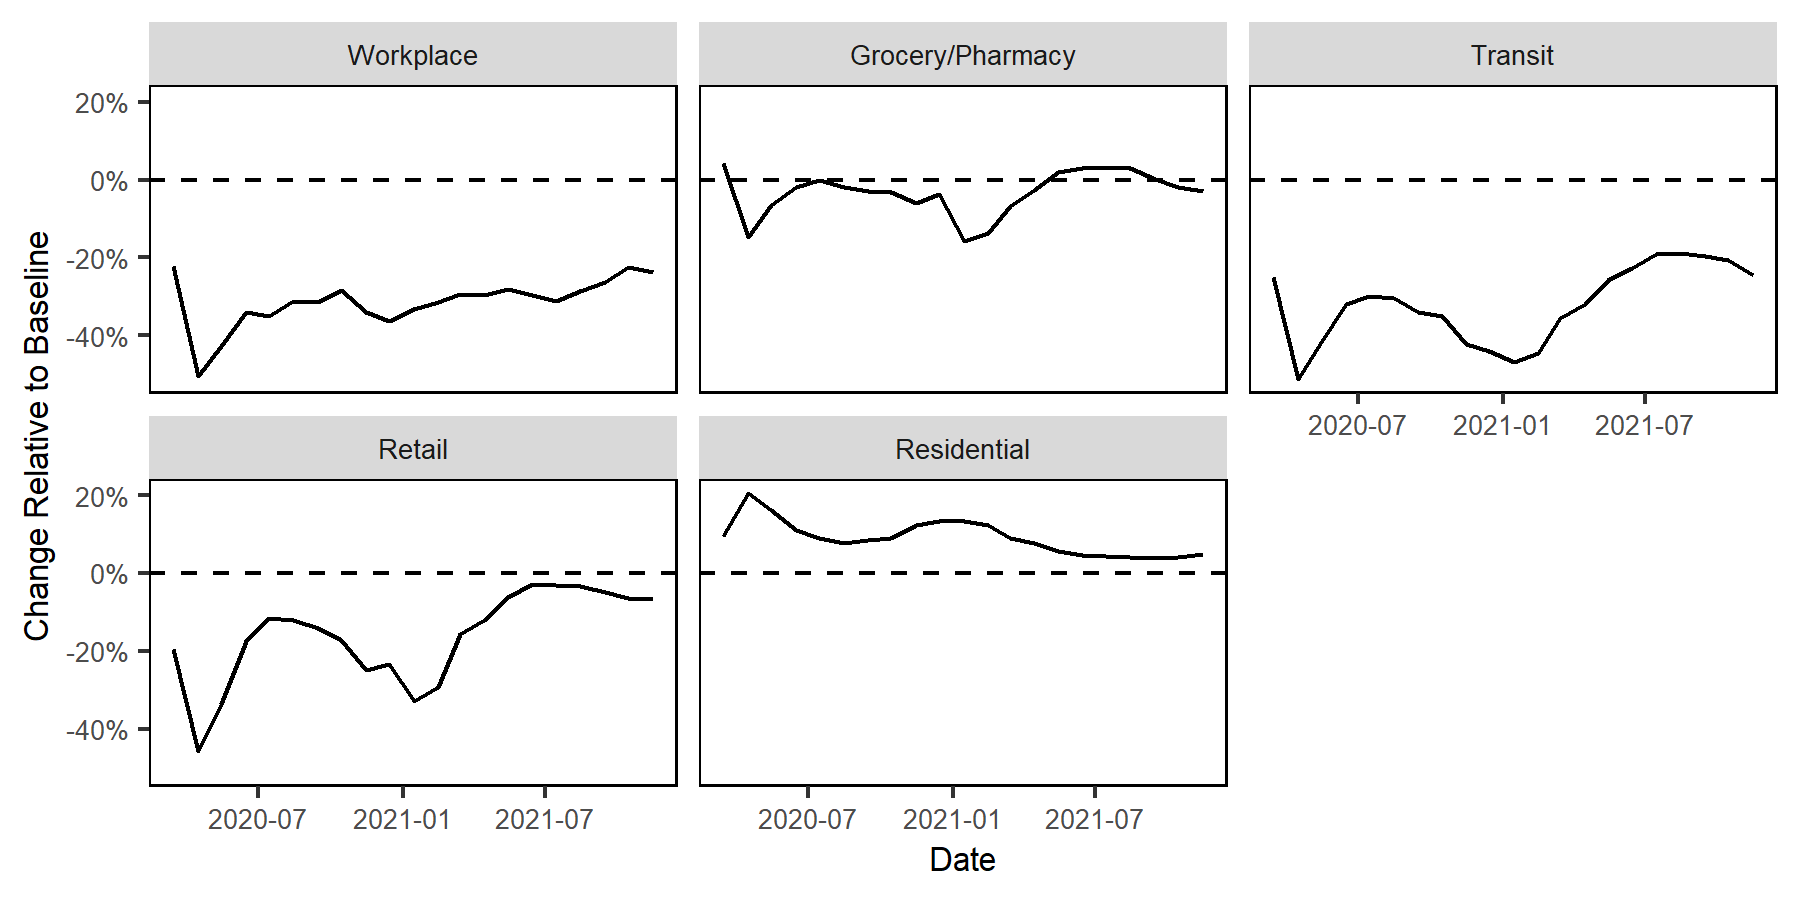
\includegraphics[width=\textwidth]{images/mobility/raw_monthly}
\end{figure}

We normalized the monthly changes by dividing the change in each month by the maximal change in any month (in practice, this was April, 2020) and truncated to be greater than zero. This yielded a proportion (bounded between 0 and 1) representing the degree to which mobility changed for each geographic category in each month, relative to the most it changed for any month. For each month, we averaged the five proportions (for five categories) to yield a single statistic, bounded on [0,1], represented the aggregate change in mobility for that month. This is shown in figure \ref{normalized_mobility}

\begin{figure}[H] 
	\caption{Normalized Community Mobility Data for the Chicago-Naperville-Elgin, IL-IN-WI Metropolitan Statistical Area}\label{normalized_mobility}
	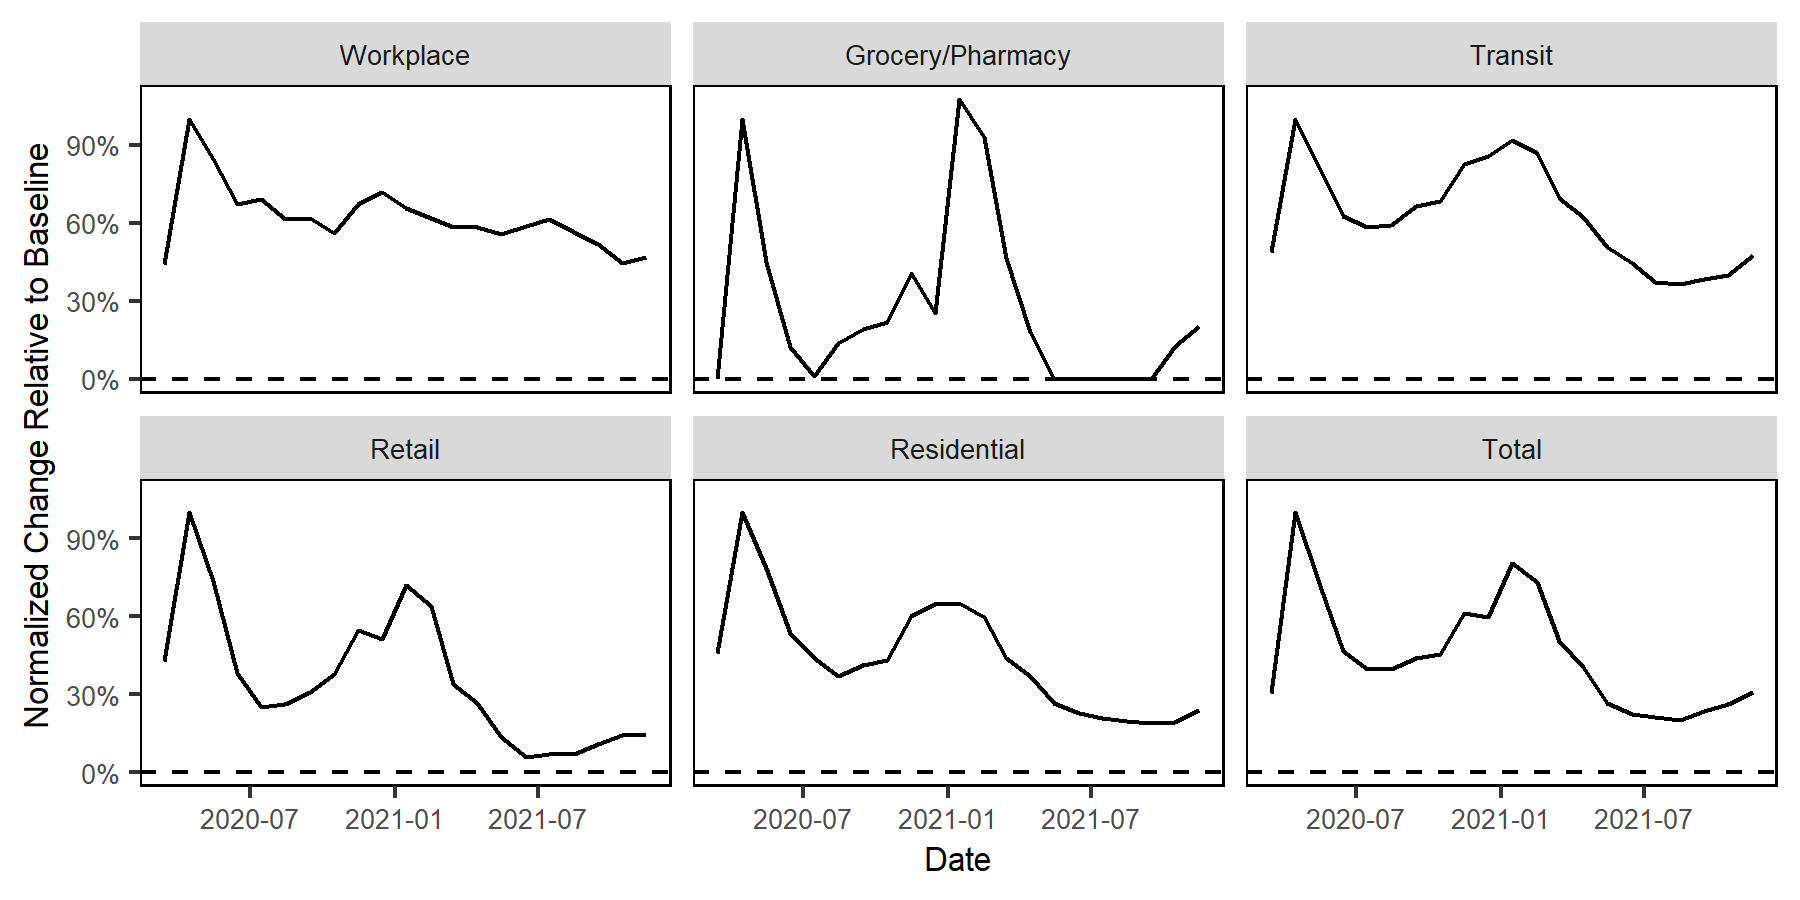
\includegraphics[width=\textwidth]{images/mobility/normalized_monthly}
\end{figure}

We combined the monthly aggregate change in mobility - denoted $\delta_t$ for month $t$ - with randomly sampled maximal reduction in each parameter - denoted $\gamma^\prime$. If we assumed that the reduction in a parameter (eg, viral suppression) - denoted $\gamma_t$ - correlated perfectly with the change in aggregate mobility, then we could multiply the monthly mobility by the sampled maximal change: 
\begin{equation*}
\gamma_t = \gamma^\prime \times \delta_t
\end{equation*}

Conversely, if the monthly reduction in a parameter were static and unrelated to mobility, we could postulate:
\begin{equation*}
\gamma_t = \gamma^\prime
\end{equation*}

Because it is unclear how much mobility patterns mirror patterns in sexual transmission, viral suppression, HIV testing, and PrEP use, we postulated that there was a weight, $w$, bounded on [0,1], which determined how much mobility influenced the monthly reduction in each parameter:

\begin{equation*}
\gamma_t = w \times \gamma^\prime \times \delta_t + (1-w) \times \gamma^\prime
\end{equation*}

Across simulations, we randomly sampled the weight parameter from a $Beta(2,2)$ distribution.

Lastly, we presumed that, after some point in time, $gamma_t$ tapered to zero over a period of several months. For sexual transmission, and for suppression, testing, and PrEP use in the "Rapid Resumption of Care" scenario, this happened from March 8, 2021 to July 4, 2021. For suppression, testing, and PrEP use in the "Prolonged Barriers to Care" scenario, this took place from Sept 8, 2021 to Jan 4, 2022. 

This was achieved by multiplying by a factor $\theta_t$. Prior to the beginning of the tapering period, $\theta_t = 1$ and after its end, $\theta_t = 0$, and decreases linearly from 1 to 0 over the course of the tapering period.

\begin{equation*}
\gamma_t = \theta_t \big [w \times \gamma^\prime \times \delta_t + (1-w) \times \gamma^\prime \big]
\end{equation*}

Figure \ref{mobility_eg} illustrates the monthly reduction in viral suppression, under both scenarios, if the sampled maximal reduction were 25\%, under three values of the weight given to mobility data (1, 0.5, and 0), for the 

\begin{figure}[H] 
	\caption{Example Monthly Reduction in Viral Suppression Given Different Weights to Mobility Data, Chicago-Naperville-Elgin, IL-IN-WI Metropolitan Statistical Area}\label{mobility_eg}
	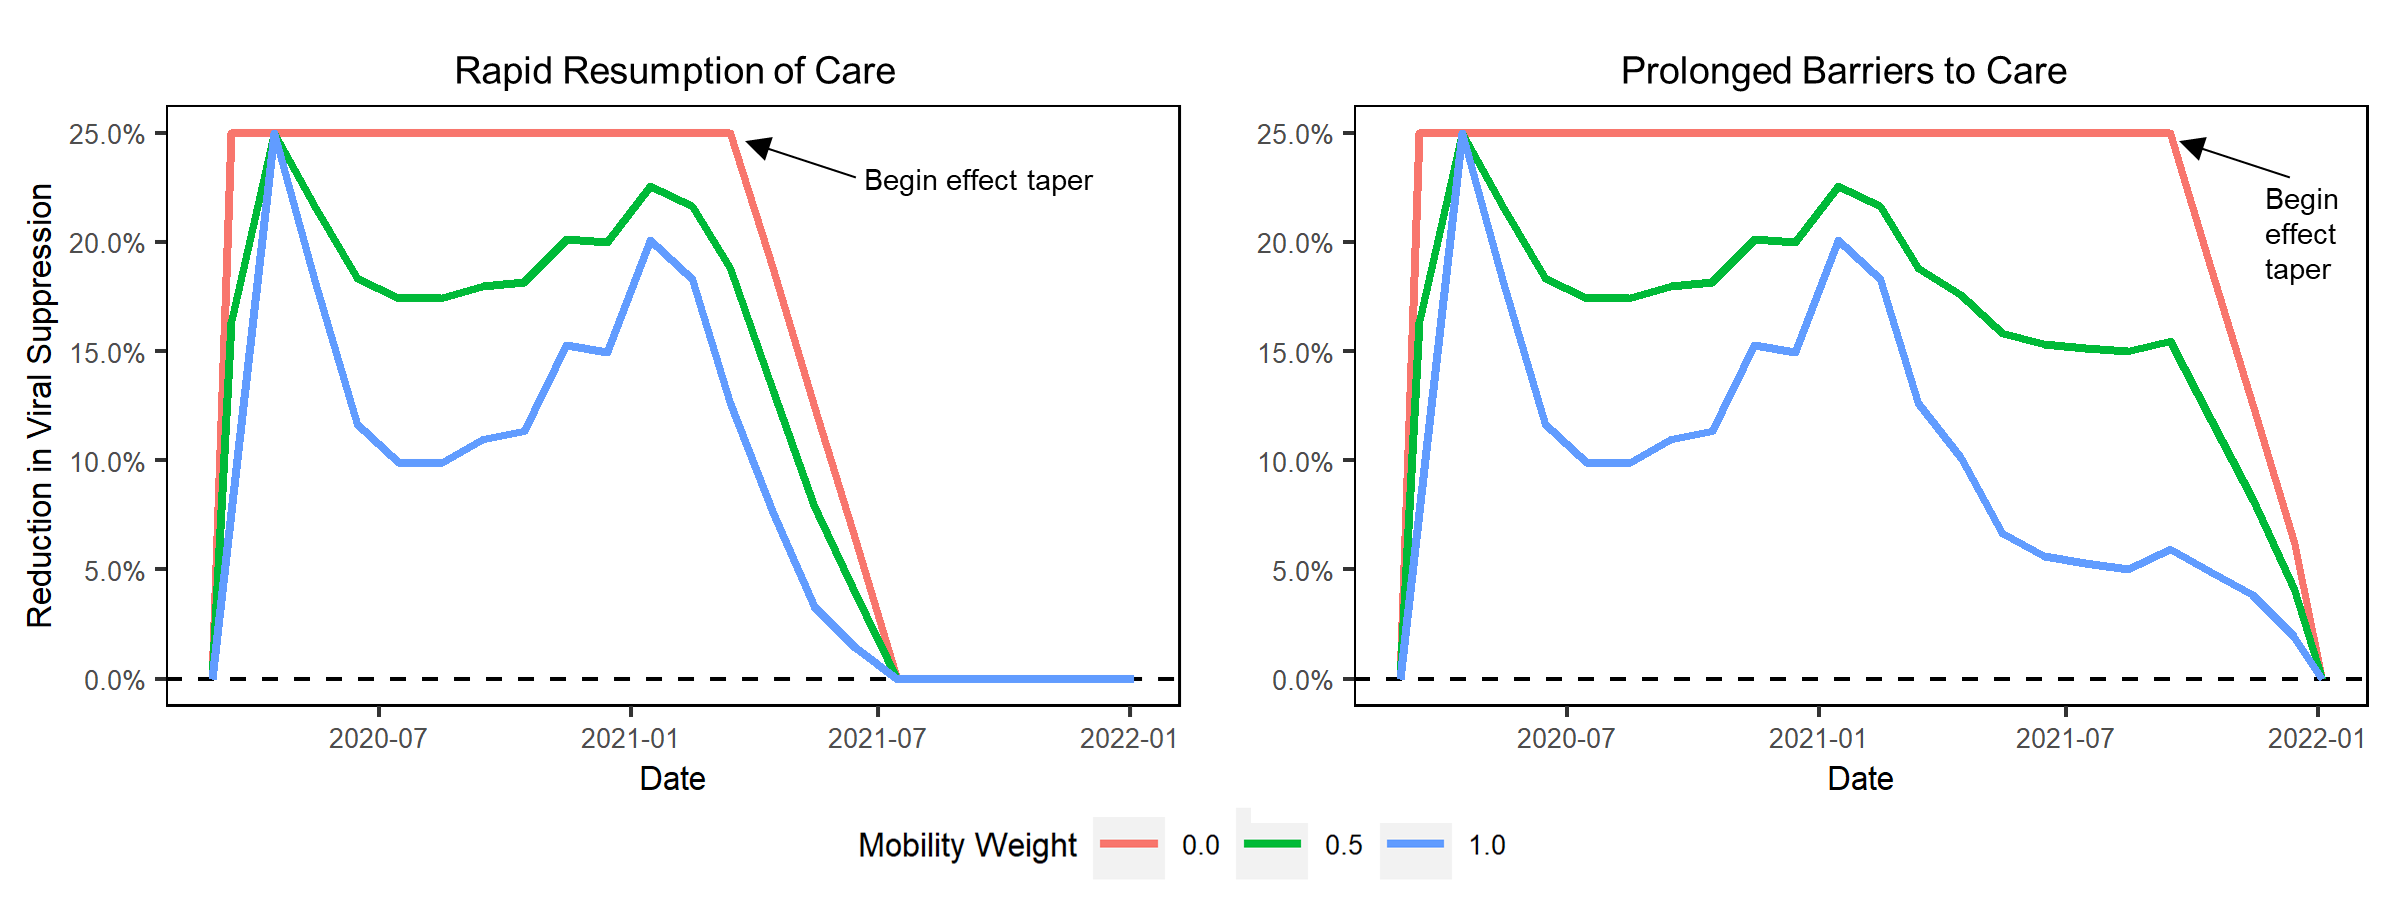
\includegraphics[width=\textwidth]{images/mobility/eg_trends}
\end{figure}
%--------------------------%
%-- SUPPLEMENTAL FIGURES --%
%--------------------------%

\newpage
\section{Additional Analyses}


\begin{figure}[H]
	\caption{Figure S4: Projected Incidence and Reported Diagnoses Under Two Scenarios Representing the Potential Effects of the COVID-19 Pandemic}
	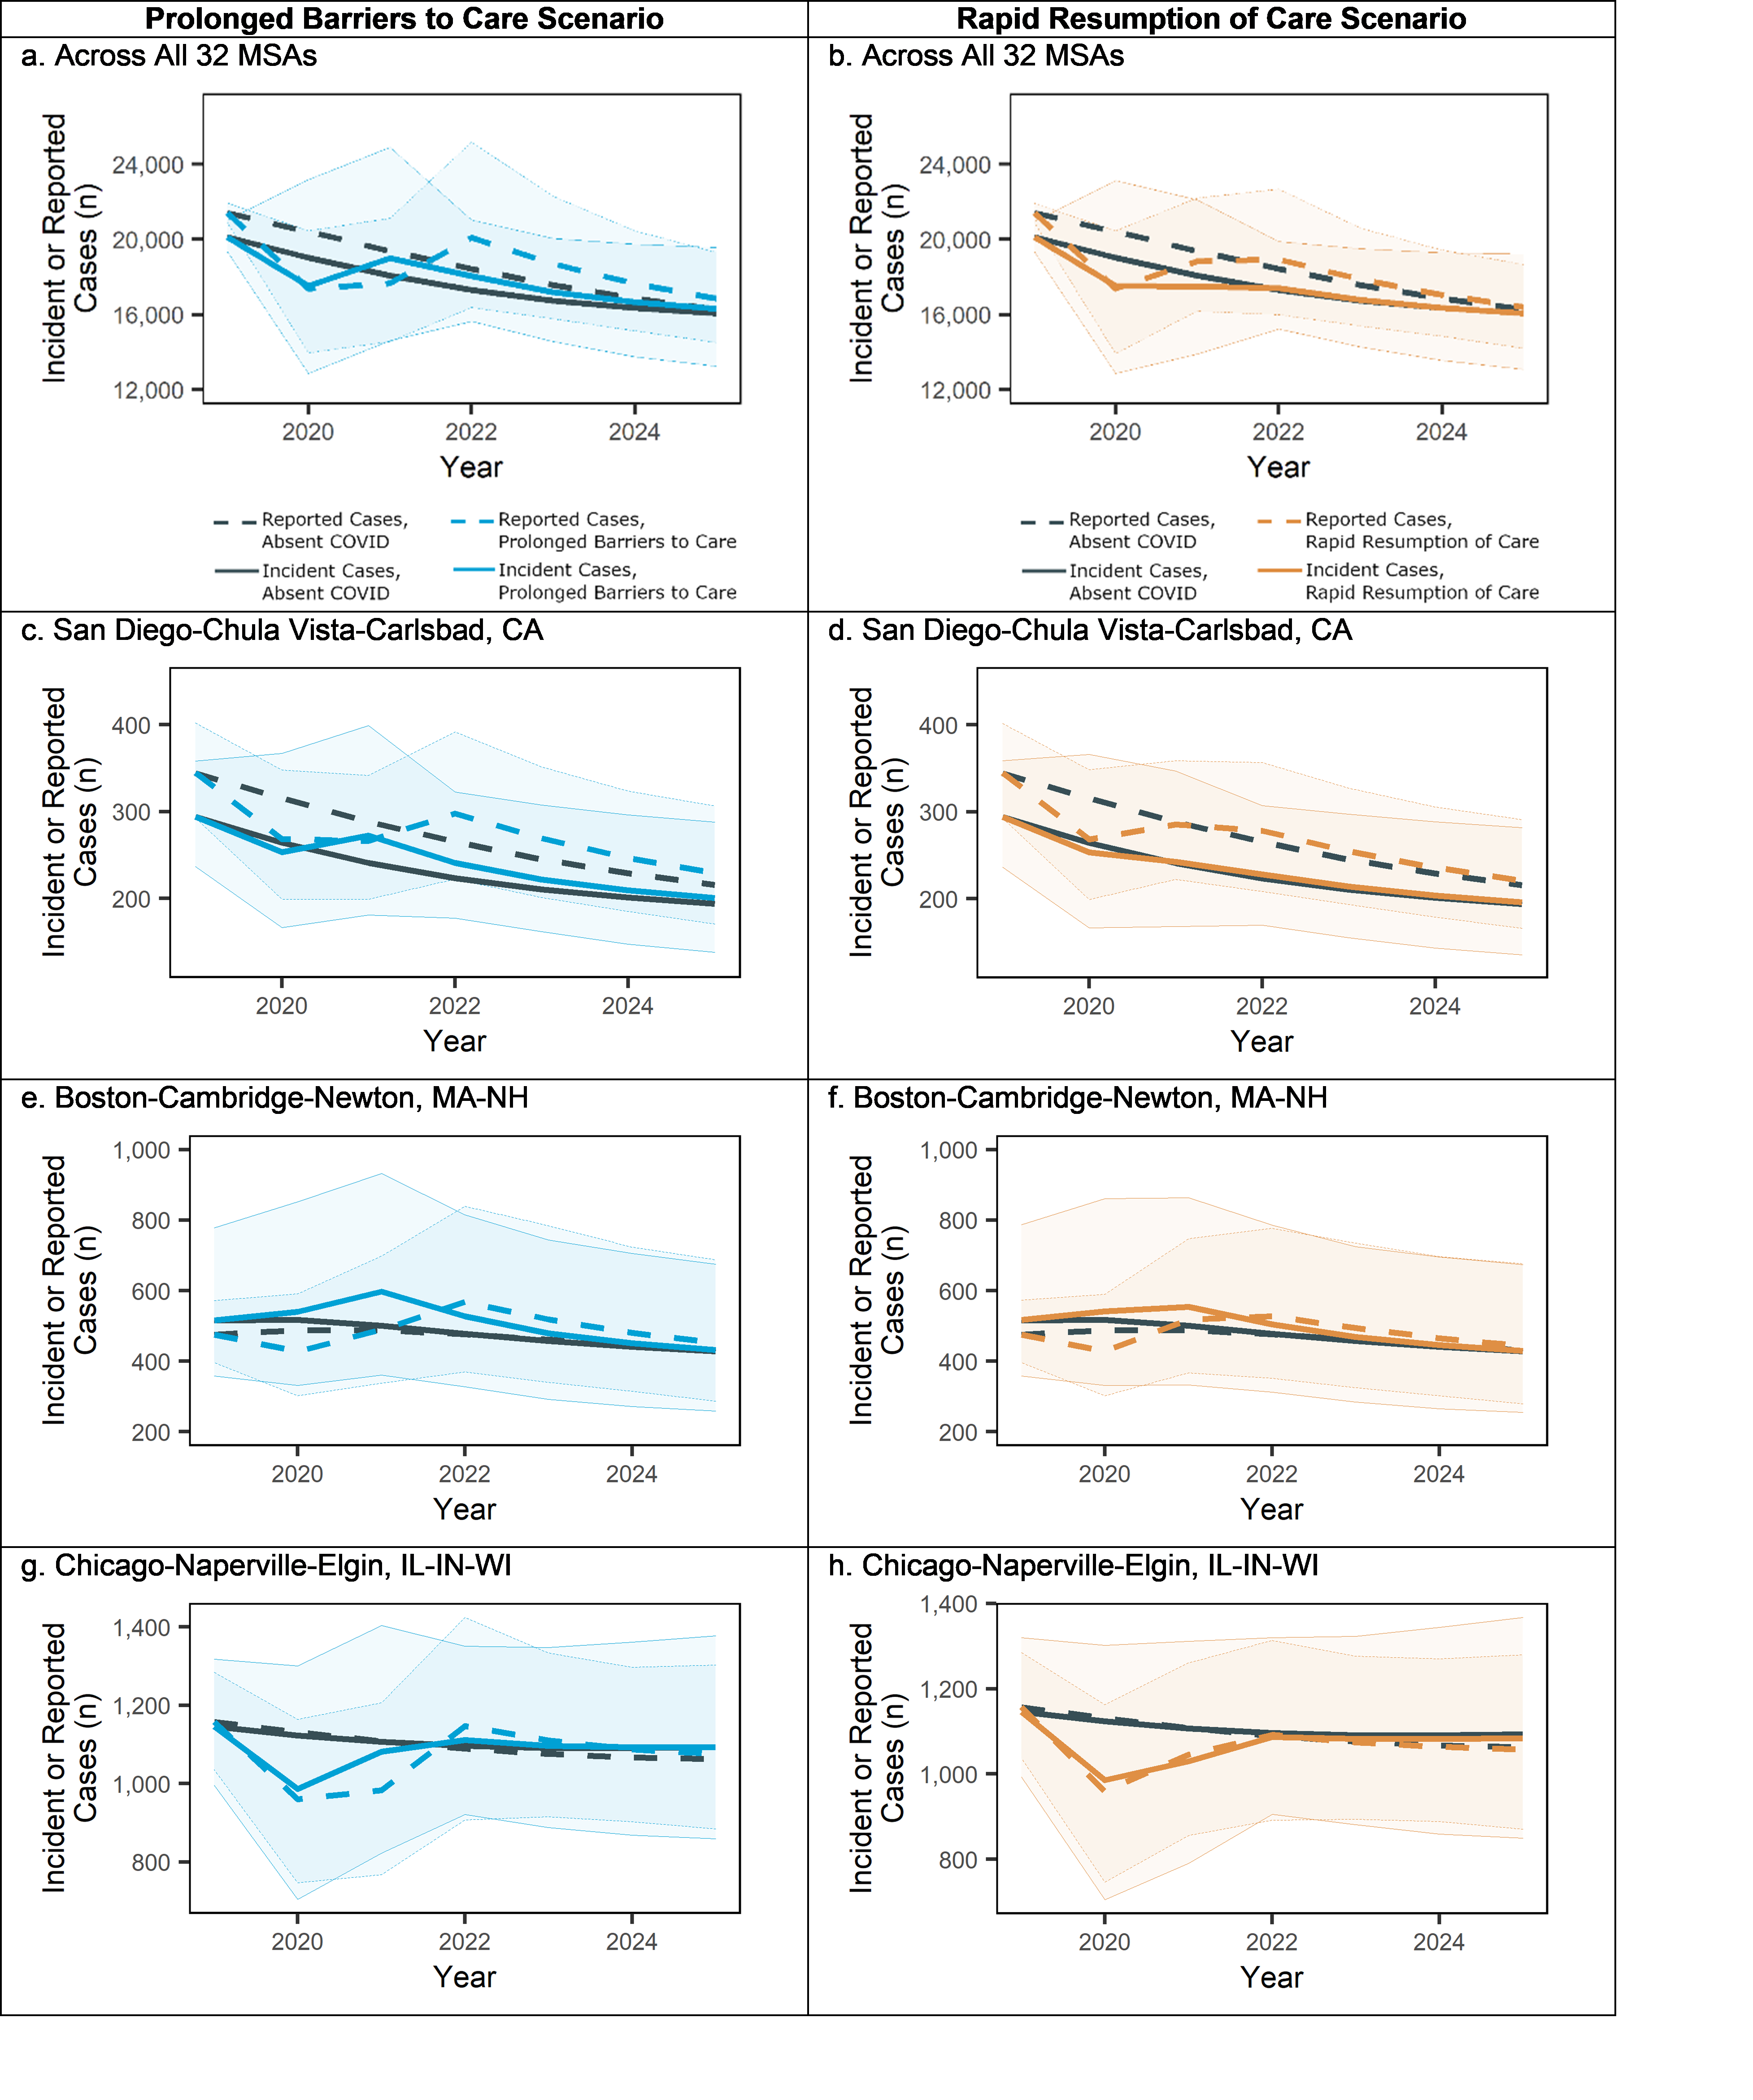
\includegraphics[width=0.85\textwidth]{images/figure_s4}
\end{figure}
Solid lines denote the mean projected incidence across 1,000 simulations, whereas dashed lines denote the mean projected reported diagnoses. The shaded ribbons indicate the 95\% credible interval. Blue lines in panels a, c, e, and g illustrate projections from the Prolonged Barriers to Care scenario (sexual transmission normalized by July 4, 2021; HIV testing, viral suppression, and PrEP use do not normalize until Feb 4, 2022); orange lines in panels b, d, f, and g illustrate the corresponding projections for the Rapid Resumption of Care scenario (sexual transmission, HIV testing, viral suppression, and PrEP use all normalize by July 4, 2021). Black lines in all panels illustrate projections if the COVID-19 pandemic had never occurred.


\begin{figure}[H]
	\caption{Relationship Between COVID Effects on Parameters and Change in Cumulative Incidence 2020-2025}
	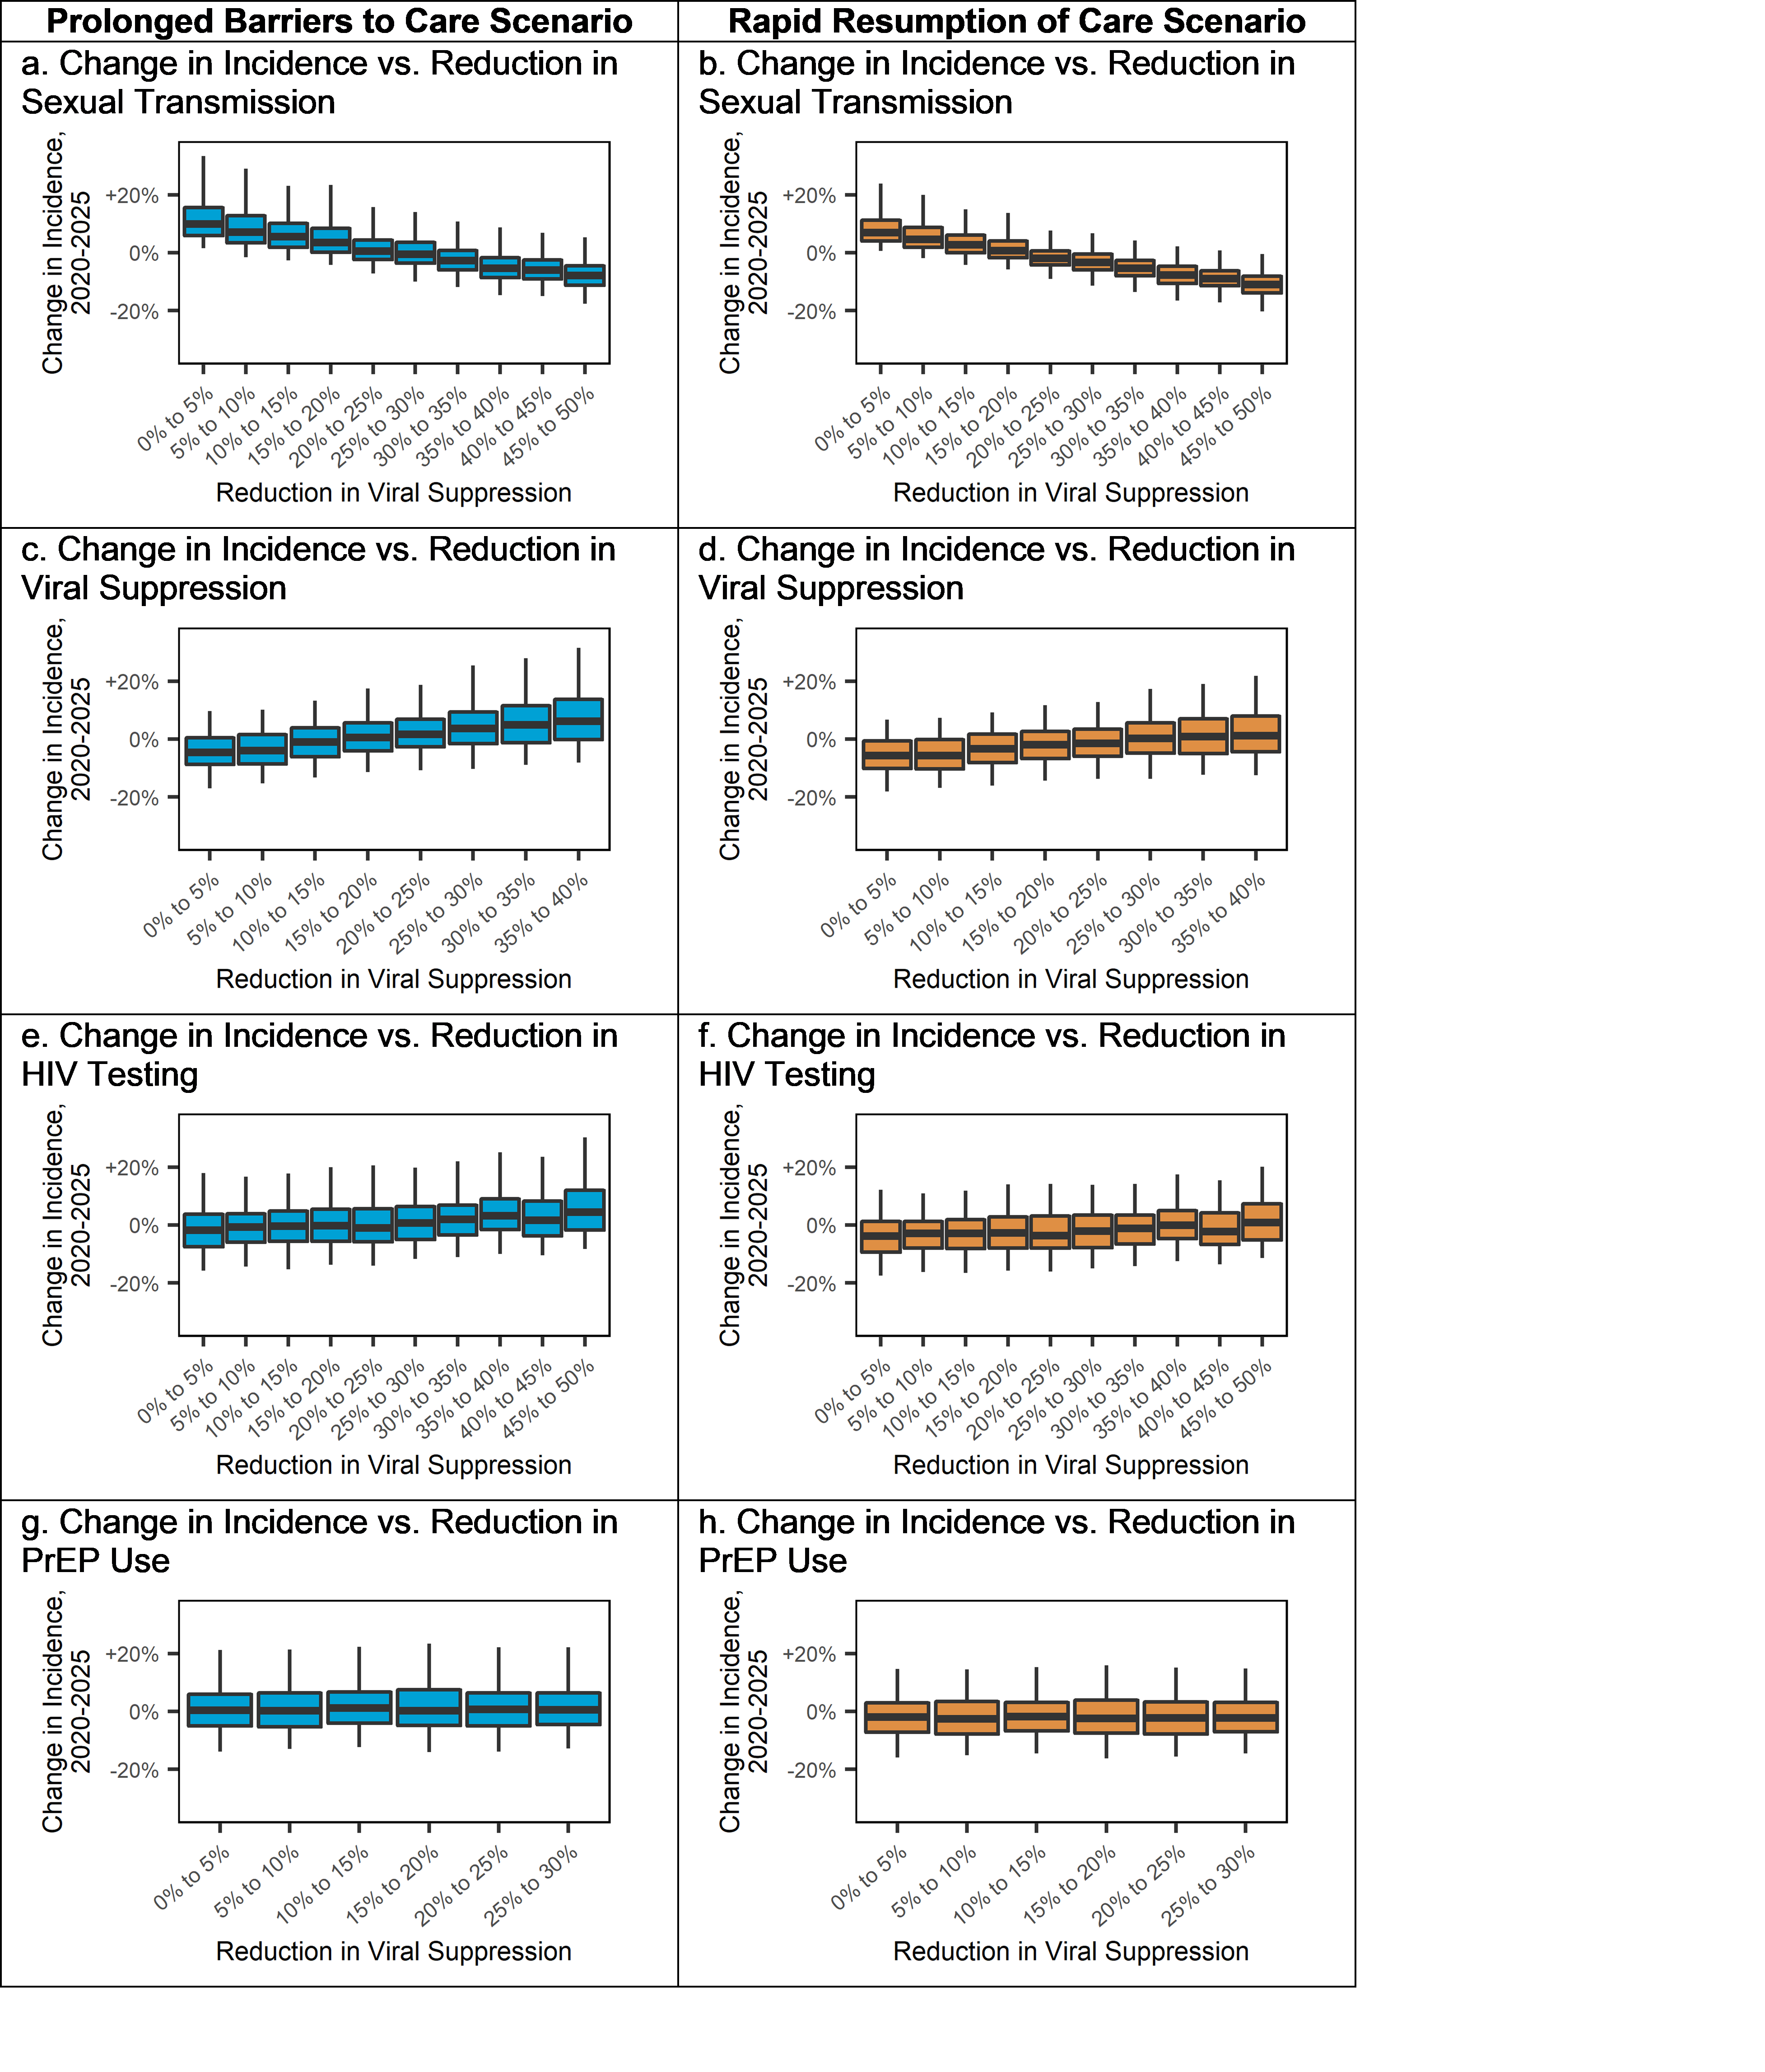
\includegraphics[width=0.85\textwidth]{images/figure_s5}
\end{figure}
The dark horizontal lines represent the median across 1,000 simulations in each of the 32 metropolitan statistical areas of the change incident cases from 2020-2025, calculated as the projected incident infections from 2020-2025 under the COVID scenario minus the incident infections if COVID had not occurred, divided by the cumulative incident infections if COVID had not occurred. The boxes denote the interquartile interval, and the whiskers denote the 95\% credible interval. Panels a, c, e, and g (blue) show projections from the Prolonged Barriers to Care scenario (sexual transmission normalized by July 4, 2021; HIV testing, viral suppression, and PrEP use do not normalize until Feb 4, 2022); Panels b, d, f, and g (orange) show the corresponding projections for the Rapid Resumption of Care scenario (sexual transmission, HIV testing, viral suppression, and PrEP use all normalize by July 4, 2021).


\begin{figure}[H]
	\caption{Strength of Association Between Cumulative HIV Incidence 2020-2025 and the Reduction in Transmission and Viral Suppression due to the COVID-19 Pandemic}
	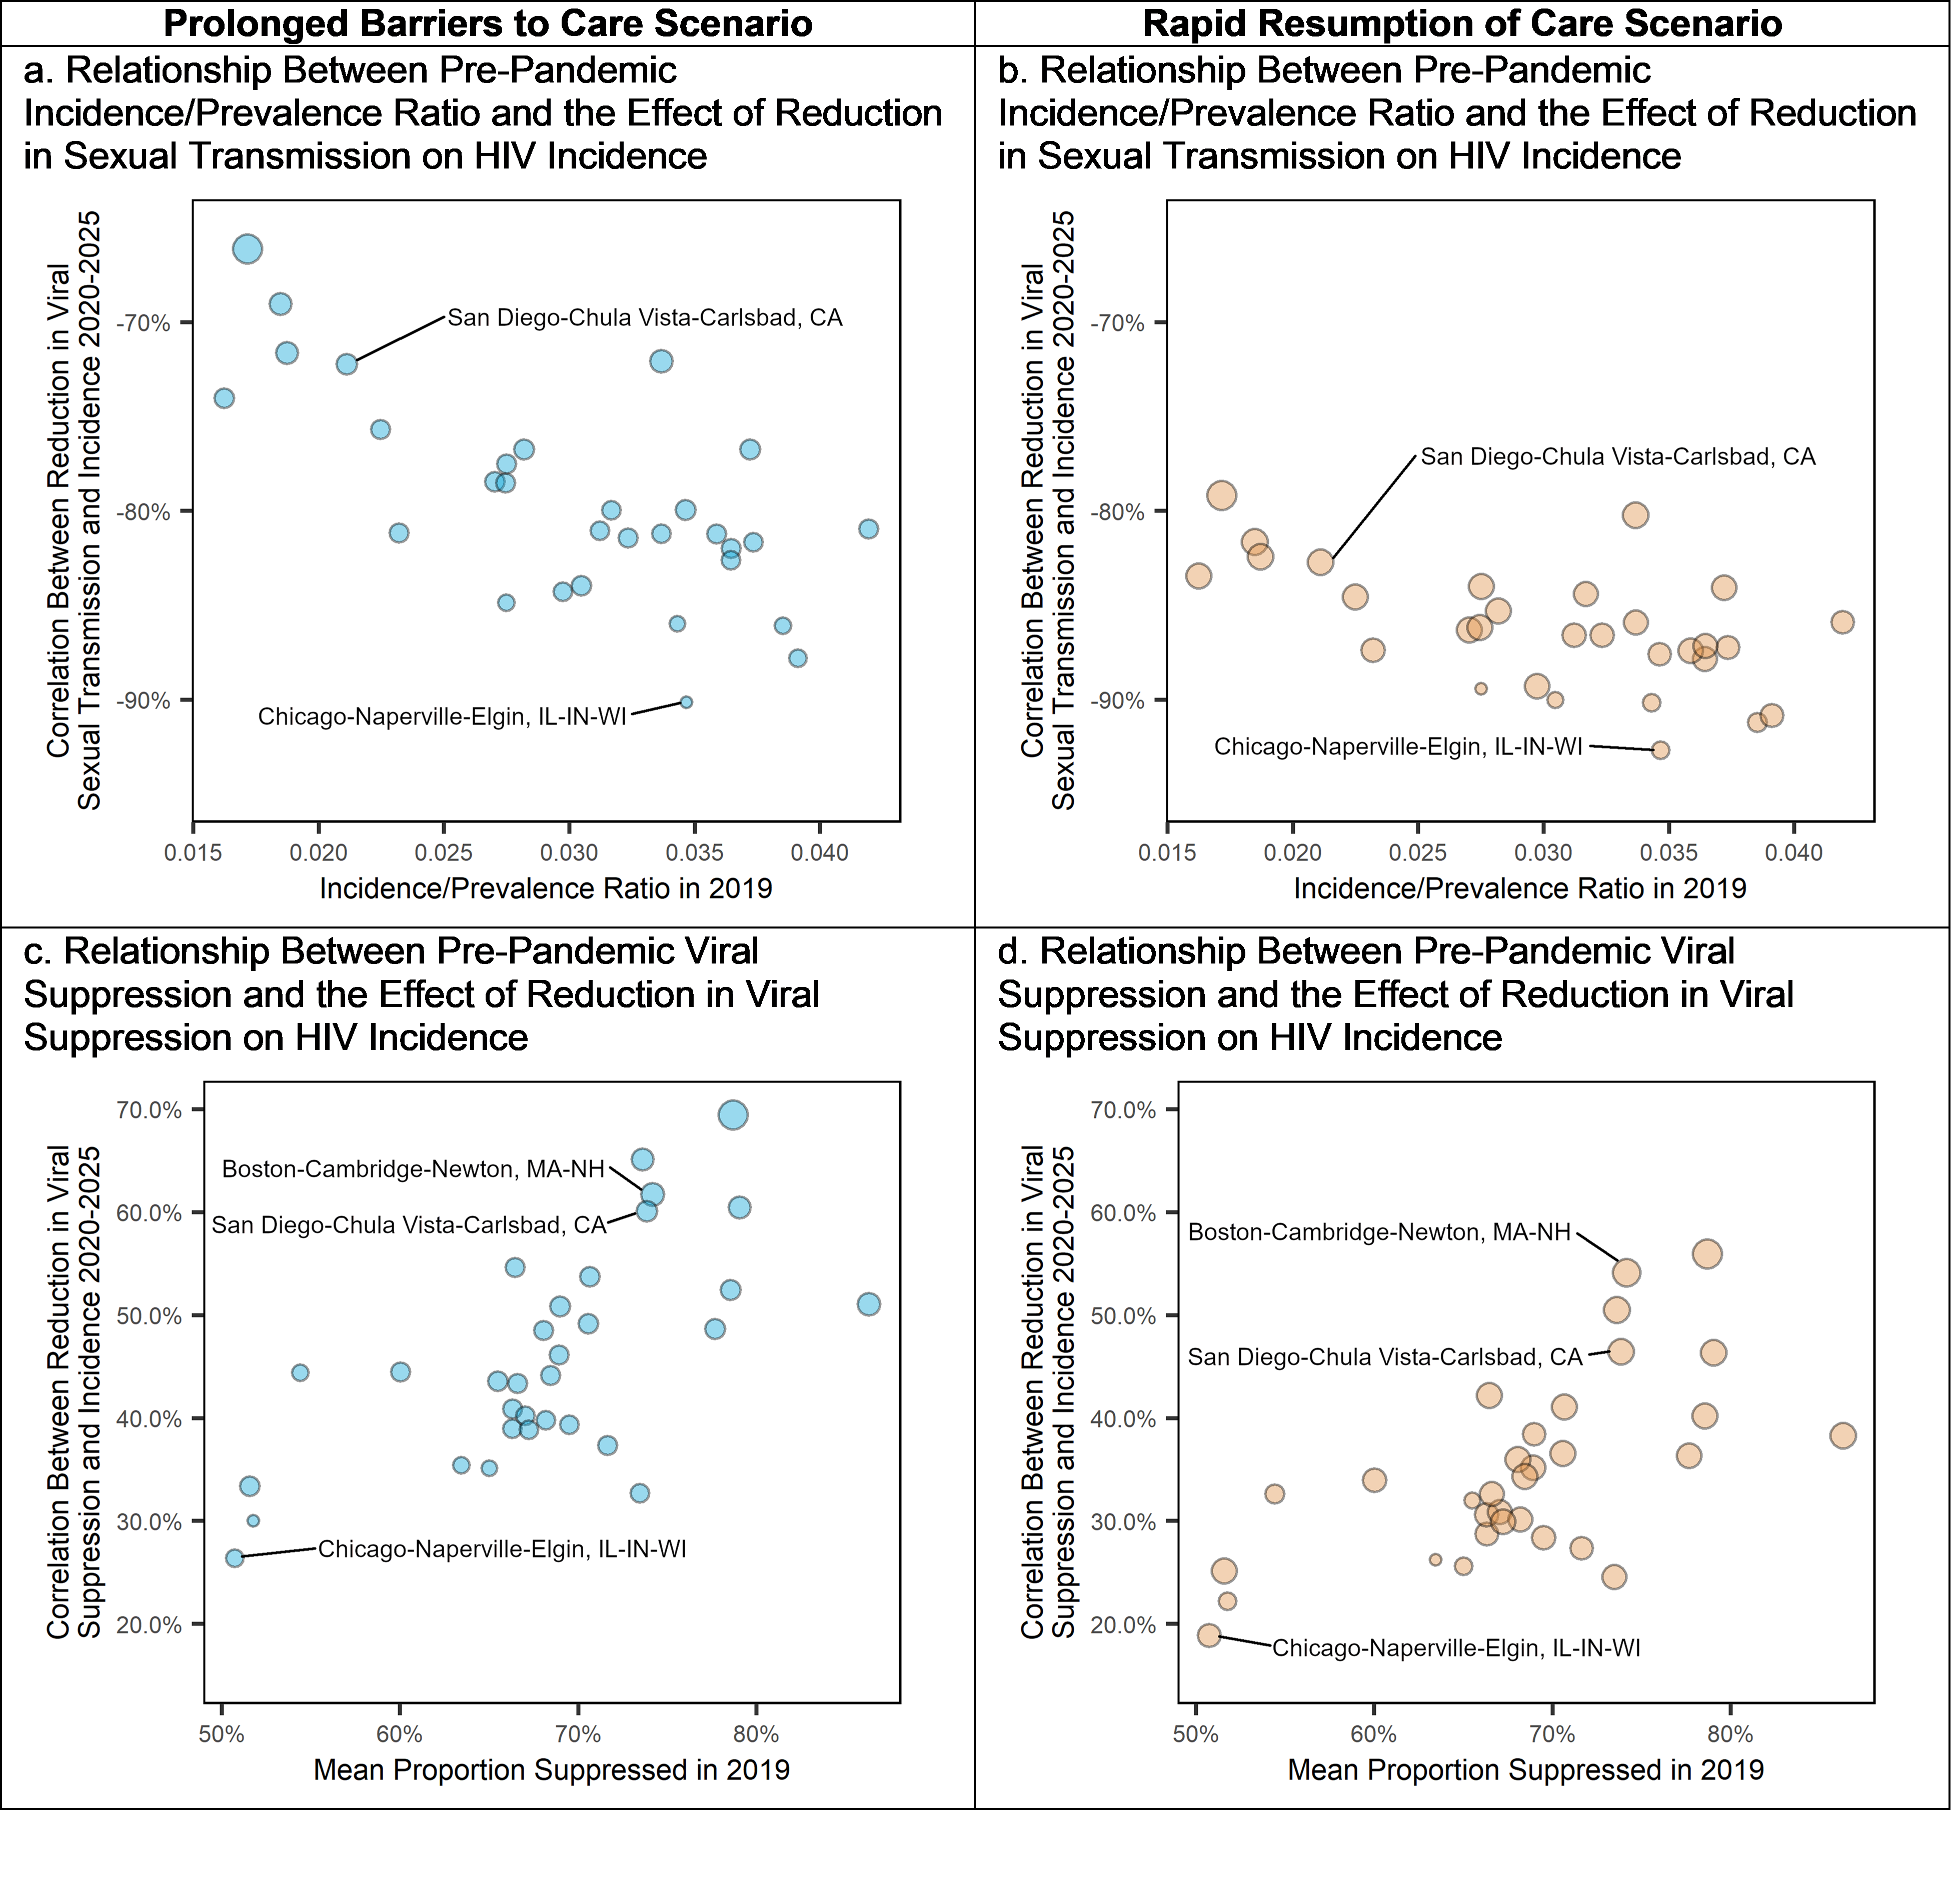
\includegraphics[width=\textwidth]{images/figure_s6}
\end{figure}
Each circle represents one metropolitan statistical area (MSA). The value on the x-axis is the mean (across 1,000 simulations in each MSA) pre-pandemic epidemiological quantity: incidence/prevalence ratio in panels a and b; proportion of diagnosed PWH who are suppressed in panels c and d. The value on the y-axis is the correlation, across all 1,000 simulations in one MSA, between the reduction sexual transmission (panels a and b) or viral suppression (panels c and d) and the relative change in cumulative incidence (under COVID vs. no COVID). The size of each circle is proportional to the relative change in cumulative incidence. Panels a and c (blue) show relationships from the Prolonged Barriers to Care scenario (sexual transmission normalized by July 4, 2021; HIV testing, viral suppression, and PrEP use do not normalize until Feb 4, 2022); Panels b and d (orange) show the corresponding relationships for the Rapid Resumption of Care scenario (sexual transmission, HIV testing, viral suppression, and PrEP use all normalize by July 4, 2021). Panels a and b do not show two outliers: Cincinnati, OH-KY-IN (Incidence/Prevalence $> 0.06$) and Boston-Cambridge-Newton, MA-NH (correlation $> -60$\%)


%%-------------------------%%
%%-- CALIBRATION TARGETS --%%
%%-------------------------%%

\newpage
\section{Calibration Targets}

\begin{table}[H]
	\caption{Model Calibration Targets}
	\small
	\begin{tabular}{r r c c c}
		\hline
		& \textbf{Target} & \textbf{Years} & \textbf{Level of Stratification} & \textbf{Data Source} \\
		\hline
		\hline
		
		\multirow{3}{*}{1.} & \multirow{3}{*}{Reported diagnoses} & \multirow{3}{*}{2009 to 2017} & sex, age, race, risk factor, & \multirow{3}{*}{CDC MSA reports \cite{hivatlas,msa2010,msa2011,msa2013,msa2014,msa2015,msa2016,cdc24.2} }\\
		& & & sex*age, sex*race, sex*race, & \\
		& & & sex*risk, race*risk & \\
		\hline
		
		\multirow{3}{*}{2.} & \multirow{3}{*}{Estimated number of diagnosed PWH} & \multirow{3}{*}{2008 to 2016} & sex, age, race, and risk factor & \multirow{3}{*}{CDC MSA reports \cite{hivatlas,msa2010,msa2011,msa2013,msa2014,msa2015,msa2016,cdc24.2} }\\
		& & & sex*age, sex*race, sex*race, & \\
		& & & sex*risk, race*risk & \\
		\hline
		
		3. & Mortality in PWH & 2009 to 2016 & sex & CDC MSA reports  \cite{msa2010,msa2011,msa2013,msa2014,msa2015,msa2016,cdc24.2} \\
		\hline
		
		\multirow{2}{*}{4}. & The proportion of PWH aware & \multirow{2}{*}{2010 to 2018} & \multirow{2}{*}{total} & \multirow{2}{*}{HIV Atlas \cite{hivatlas} }\\
		& of their diagnosis (state-level) & & & \\
		\hline
		
		\multirow{2}{*}{5.} & The proportion of diagnosed PWH & \multirow{2}{*}{2010 to 2018} & total + age, race, sex, & \multirow{2}{*}{local health departments} \\
		& who were virally suppressed & & risk factor (when available) & \\
		\hline
		
		\multirow{3}{*}{6.} & The number of individuals & \multirow{3}{*}{2010 to 2018} & \multirow{3}{*}{sex, race} & \multirow{3}{*}{AIDSVu \cite{aidsvu_prep} }\\
		& receiving a prescription for & & & \\
		& emtricitabine/tenofovir for PrEP & & & \\
		\hline
		
		7. & The proportion receiving an HIV test & 2013 to 2017 & age, sex, race & BRFSS \cite{brfss.13.17} \\
		\hline
		
		\multirow{2}{*}{8.} & The prevalence of injection drug use & \multirow{2}{*}{2014 to 2016} & \multirow{2}{*}{age} & \multirow{2}{*}{NSDUH \cite{nsduh} }\\
		& (sub-state estimates) & & & \\
		\hline
		
		9. & Cumulative AIDS mortality & up to 2002 & age, race, sex, risk factor & AIDS Public Information Dataset\cite{apids} \\
		\hline
		
		10. & Reported AIDS diagnoses & 1998 to 2002 & total &  AIDS Public Information Dataset\cite{apids} \\
		\hline		
	\end{tabular}
\end{table}


%---------------------------------%
%-- PARAMETERS --%
%---------------------------------%
\newpage
\section{Model Parameters and Their Prior Distributions}
\tabulinesep=2pt
%\begin{longtable}{| p{.45\textwidth} | c{.09\textwidth} | p{.13\textwidth} | p{.08\textwidth} | p{.25\textwidth} |}
\begin{longtabu} to \textwidth {|X[45,l,m]|X[9,c,m]|X[13,c,m]|X[8,c,m]|X[25,l,m]|}

%-- TABLE SET-UP --%
	\caption{Model Parameters and Sampling Distributions.\label{params_tab}}\\
	
	\hline
%	\multicolumn{2}{| c |}{Table S1: Model Parameters}\\
%	\hline
	\textbf{Parameter} & \textbf{Estimate} & \textbf{Uncertainty Range} & \textbf{Symbol/ Section} & \textbf{References} \\
	\hline
	\hline
	\endfirsthead
	
	\hline
	\multicolumn{5}{|l|}{Table \ref{params_tab} (Model Parameters) continued}\\
	\hline
	\textbf{Parameter} & \textbf{Estimate} & \textbf{Uncertainty Range} & \textbf{Symbol/ Section} & \textbf{References} \\
	\hline
	\hline
	\endhead
	
	\hline
	\hline
	\multicolumn{5}{|l|}{\textit{*Uncertainty Range represents the 95\% confidence interval for a Lognormal distribution unless otherwise indicated}}\\
	\hline
	\endfoot
	
%	\hline
%	\multicolumn{2}{| c |}{End of Table}\\
	\hline\hline
	\endlastfoot
	

%----------------------------%	
%-- HIV TRANSMISSION RATES --%
%----------------------------%

	\multicolumn{5}{|l|}{\textbf{HIV TRANSMISSION RATES}}\\ \hline
	
%	Global Transmission Rate & 1 & \textit{improper uniform on log scale} & $\gamma_0$ (\ref{trates}) & \\ \hline
	
	\multicolumn{5}{|l|}{\textbf{Male-to-male Sexual Transmission}}\\ 
	\multicolumn{5}{|l|}{\textit{(A composite of number of sexual encounters and rate of transmission per encounter)}}\\ \hline
	Black, 2000 & 1 & [0.003 - 354] & $\omega^{(MSM)}$ & \\ \cline{1-3}
	Black, ratio of rate by 2010 to 2000 rate & 1 & [0.257 - 3.891] & \ref{trates} & \\ \cline{1-3}
	Black, ratio of rate by 2020 to 2010 rate & 1 & [0.507 - 1.972] & & \\ \cline{1-3}
	Hispanic, 2000 & 1 & [0.003 - 354] & & \\ \cline{1-3}
	Hispanic, ratio of rate by 2010 to 2000 rate & 1 & [0.257 - 3.891] & & \\ \cline{1-3}
	Hispanic, ratio of rate by 2020 to 2010 rate & 1 & [0.507 - 1.972] & & \\ \cline{1-3}
	Non-Black/Non-Hispanic, 2000 & 1 & [0.003 - 354] & & \\ \cline{1-3}
	Non-Black/Non-Hispanic, ratio of rate by 2010 to 2000 rate & 1 & [0.257 - 3.891] & & \\ \cline{1-3}
	Non-Black/Non-Hispanic, ratio of rate by 2020 to 2010 rate & 1 & [0.507 - 1.972] & & \\ \cline{1-3} \cline{5-5}
	Ratio of rate before 1980 to rate by 2000 (All Races) & 3.1 & [0.404 - 23.790] & & HIV Atlas\cite{hivatlas}\\ \hline
	
	\multicolumn{5}{|l|}{\textbf{Heterosexual Transmission}}\\  
	\multicolumn{5}{|l|}{\textit{(A composite of number of sexual encounters and rate of transmission per encounter)}}\\ \hline
	Black, 2000 & 1 & [0.003 - 354] & $\omega^{(het)}$& \\ \cline{1-3}
	Black, ratio of rate by 2010 to 2000 rate & 1 & [0.257 - 3.891] & \ref{trates} & \\ \cline{1-3}
	Black, ratio of rate by 2020 to 2010 rate & 1 & [0.507 - 1.972] & & \\ \cline{1-3}
	Hispanic, 2000 & 1 & [0.003 - 354] & & \\ \cline{1-3}
	Hispanic, ratio of rate by 2010 to 2000 rate & 1 & [0.257 - 3.891] & & \\ \cline{1-3}
	Hispanic, ratio of rate by 2020 to 2010 rate & 1 & [0.507 - 1.972] & & \\ \cline{1-3}
	Non-Black/Non-Hispanic, 2000 & 1 & [0.003 - 354] & & \\ \cline{1-3}
	Non-Black/Non-Hispanic, ratio of rate by 2010 to 2000 rate & 1 & [0.257 - 3.891] & & \\ \cline{1-3}
	Non-Black/Non-Hispanic, ratio of rate by 2020 to 2010 rate & 1 & [0.507 - 1.972] & & \\ \cline{1-3} \cline{5-5}
	Ratio of rate before 1980 to rate by 2000 (All Races) & 2.2 & [0.287 - 16.883] & & HIV Atlas \cite{hivatlas}\\ \hline
	
	\multicolumn{5}{|l|}{\textbf{Transmission via Needle Sharing}}\\  
	\multicolumn{5}{|l|}{\textit{(A composite of number of needle-sharing encounters and rate of transmission per encounter)}}\\ \hline
	Black & 1 & [0.003 - 354] & $\omega^{(IDU)}$ & \\ \cline{1-3}
	Black, ratio of rate by 2010 to 2000 rate & 1 & [0.257 - 3.891] & \ref{trates} & \\ \cline{1-3}
	Black, ratio of rate by 2020 to 2010 rate & 1 & [0.507 - 1.972] & & \\ \cline{1-3}
	Hispanic & 1 & [0.003 - 354] & & \\ \cline{1-3}
	Hispanic, ratio of rate by 2010 to 2000 rate & 1 & [0.257 - 3.891] & & \\ \cline{1-3}
	Hispanic, ratio of rate by 2020 to 2010 rate & 1 & [0.507 - 1.972] & & \\ \cline{1-3}
	Non-Black/Non-Hispanic, 2000 & 1 & [0.003 - 354] & & \\ \cline{1-3}
	Non-Black/Non-Hispanic, ratio of rate by 2010 to 2000 rate & 1 & [0.257 - 3.891] & & \\ \cline{1-3}
	Non-Black/Non-Hispanic, ratio of rate by 2020 to 2010 rate & 1 & [0.507 - 1.972] & & \\ \cline{1-3} \cline{5-5}
	Ratio of rate before 1980 to rate by 2000 (All Races) & 4.7 & [0.612 - 36.068] & & HIV Atlas\cite{hivatlas}\\ \hline
	

%---------------------------%
%-- SUSCEPTIBILITY BY AGE --%
%---------------------------%

	\multicolumn{5}{|l|}{}\\ 
	\multicolumn{5}{|l|}{}\\ \hline
	\multicolumn{5}{|l|}{\textbf{SUSCEPTIBILTY TO HIV INFECTION BY AGE}}\\ \hline
		
	\multicolumn{5}{|l|}{\textbf{via Male-to-male Sexual Contact}}\\  
	\multicolumn{5}{|l|}{\textit{(A composite of probability of being sexually active, number of encounters, and rate of transmission per encounter)}}\\ \hline
	Age 13-24 prior to 2010 (relative to age 35-44) & 0.67 & [0.48 - 0.94] & $\omega^{(A)}$ & Twenge 2017\cite{twenge2017} \\ \cline{1-3}
	Age 13-24 by 2020 (relative to age 35-44) & 0.67 & [0.48 - 0.94] & (\ref{trates}) &  Abma 2017\cite{abma2017} \\ \cline{1-3}
	Age 25-34 prior to 2010 (relative to age 35-44)	& 1.11 & [0.79 - 1.56] &&\\ \cline{1-3}
	Age 25-34 by 2020 (relative to age 35-44) & 1.11 & [0.79 - 1.56] &&\\ \cline{1-3}
	Age 45-54 (relative to age 35-44) & 0.72 & [0.51 - 1.01] &&\\ \cline{1-3}
	Age 55+ (relative to age 35-44) & 0.35 & [0.25 - 0.49] &&\\ \hline

	\multicolumn{5}{|l|}{\textbf{via Heterosexual Contact}}\\   
	\multicolumn{5}{|l|}{\textit{(A composite of probability of being sexually active, number of encounters, and rate of transmission per encounter)}}\\ \hline
	Age 13-24 (relative to age 35-44) & 0.67 & [0.48 - 0.94] & $\omega^{(A)}$ & Twenge 2017\cite{twenge2017} \\ \cline{1-3}
	Age 25-34 (relative to age 35-44) & 1.11 & [0.79 - 1.56] & (\ref{trates}) & Abma 2017\cite{abma2017} \\ \cline{1-3}
	Age 45-54 (relative to age 35-44) & 0.72 & [0.51 - 1.01] &&	\\ \cline{1-3}
	Age 55+ (relative to age 35-44) & 0.35 & [0.25 - 0.49] &&\\ \hline	

	\multicolumn{5}{|l|}{\textbf{via Needle Sharing}}\\   
	\multicolumn{5}{|l|}{\textit{(A composite of number of needle-sharing encounters and rate of transmission per encounter)}}\\ \hline
	Age 13-24 (relative to age 35-44) & 1.04 & [0.74 - 1.46] & $\omega^{(A)}$ & HIV Surveillance \#24\cite{nhbs24}\\ \cline{1-3}
	Age 25-34 (relative to age 35-44) & 1.06 & [0.75 - 1.49] & (\ref{trates}) & \\ \cline{1-3}	
	Age 45-54 (relative to age 35-44) & 0.84 & [0.60 - 1.18] &&\\ \cline{1-3}
	Age 55+ (relative to age 35-44) & 0.70 & [0.50 - 0.98] &&\\ \hline
	
%-----------------------------%
%-- RELATIVE SUSCEPTIBILITY --%
%-----------------------------%

\multicolumn{5}{|l|}{}\\ \hline
\multicolumn{5}{|l|}{\textbf{RELATIVE SUSCEPTIBILITY TO HIV ACQUISITION}}\\ \hline
	
	via needle sharing, MSM-IDU vs heterosexual male prior to 1990 & 3.30 & [1.67 - 6.51] & & Strathdee 1997 \cite{strathdee1997} \\ \cline{1-3}
	via needle sharing, MSM-IDU vs heterosexual male by 2000 & 3.30 & [1.67 - 6.51] & &\\ \cline{1-3}	
	via needle sharing, MSM-IDU vs heterosexual male by 2010 & 3.30 & [1.67 - 6.51] & &\\ \cline{1-3}	
	via needle sharing, MSM-IDU vs heterosexual male by 2020 & 3.30 & [1.67 - 6.51] & &\\ \hline
	via needle sharing, female vs heterosexual male & 1.10 & [0.56 - 2.17] && HIV Surveillance \#24 \cite{nhbs24} \\ \hline
	via heterosexual contact, male vs female & 0.75 & [0.38 - 1.48] && Shah 2016 \cite{shah2016}, NHBS Report \#19 \cite{nhbs19}\\	\hline
	
%----------------------%
%-- TRANSMISSIBILITY --%
%----------------------%

\multicolumn{5}{|l|}{}\\ \hline
\multicolumn{5}{|l|}{\textbf{TRANSMISSIBILITY OF HIV BY HIV NATURAL HISTORY AND CARE/TREATMENT ENGAGEMENT}}\\ \hline

	Relative Risk of Transmission for Acute vs Chronic HIV & 12 & [8.54 - 16.85] & & Shah 2016 \cite{shah2016}\\ \hline
	Relative Risk of Transmission by PWH with diagnosed vs undiagnosed HIV & 0.3 & [0.21 - 0.42] & & Marks 2005 \cite{marks2005}, Marks 2006 \cite{marks2006}\\ \hline
	Relative Risk of Transmission by PWH virally suppressed vs unsuppressed & 0 & \textit{Not Sampled} & & Eisinger 2019 \cite{eisinger2019}\\ \hline
	
%--------------------------%
%-- SEXUAL ASSORTATIVITY --%
%--------------------------%

	\multicolumn{5}{|l|}{}\\ \hline
	\multicolumn{5}{|l|}{\textbf{SEXUAL ASSORTATIVITY}}\\ \hline
	
	Proportion of female sexual partnerships with MSM, relative to the proportion of MSM in the population & 0.0895 & [0.045 - 0.177] & & Pathela 2006 \cite{pathela2006}\\ \hline
	Proportion of heterosexual male partnerships with other males & 0.004 & [0.002 - 0.008] & & Pathela 2006\cite{pathela2006}\\ \hline
	Proportion of non-IDU sexual partnerships with active IDU, relative the the prevalence of active IDU in the population & 0.2 & [0.10 - 0.39] & & Jenness 2010\cite{jenness2010}\\ \hline
	Proportion of Black sexual partnerships with Black partners, relative to the proportion Black in the population & 3.76 & [2.68 - 5.28] & & Bohl 2011\cite{bohl2011}\\ \hline
	Proportion of Hispanic sexual partnerships with Hispanic partners, relative to the proportion Hispanic in the population & 2.19 & [1.56 - 3.08] & & Mutanski 2014 \cite{mutanski2014}\\ \hline
	Proportion of Non-Black/Non-Hispanic sexual partnerships with Non-Black/Non-Hispanic partners, relative to the proportion Other in the population & 1.55 & [1.10 - 2.18] & & Fujimoto 2015 \cite{fujimoto2015}, Hamilton 2015 \cite{hamilton2015}\\ \hline
	Dispersion of age of sexual partnerships & \textit{Sex- and age-specific} & [0.71 - 1.40] $\times$ estimate & & Chow 2016 \cite{chow2016}\\ \hline
	Ratio of proportion of 13yo who are sexually active to 20-24yo proportion & 0.101 & \textit{Not Sampled} & & Abma 2017 \cite{abma2017}\\ \cline{1-3}
	Ratio of proportion of 14yo who are sexually active to 20-24yo proportion & 0.144 & \textit{Not Sampled} & & \\ \cline{1-3}
	Ratio of proportion of 15yo who are sexually active to 20-24yo proportion & 0.173 & \textit{Not Sampled} & & \\ \cline{1-3}
	Ratio of proportion of 16yo who are sexually active to 20-24yo proportion & 0.346 & \textit{Not Sampled} & & \\ \cline{1-3}
	Ratio of proportion of 17yo who are sexually active to 20-24yo proportion & 0.546 & \textit{Not Sampled} & & \\ \cline{1-3} 
	Ratio of proportion of 18yo who are sexually active to 20-24yo proportion & 0.733 & \textit{Not Sampled} & & \\ \cline{1-3} 
	Ratio of proportion of 19yo who are sexually active to 20-24yo proportion & 0.906 & \textit{Not Sampled} & & \\ \hline
	Ratio of proportion of 65-74yo who are sexually active to 55-64yo proportion & 0.721 & \textit{Not Sampled} & & Lindau 2007 \cite{lindau2007}\\ \cline{1-3} 
	Ratio of proportion of 75+yo who are sexually active to 55-64yo proportion & 0.366 & \textit{Not Sampled} & & \\ \hline

%----------------------------------%
%-- NEEDLE SHARING ASSORTATIVITY --%
%----------------------------------%

	\multicolumn{5}{|l|}{}\\ \hline
	\multicolumn{5}{|l|}{\textbf{NEEDLE SHARING ASSORTATIVITY}}\\ \hline
	
	Proportion of Black needle-sharing partnerships with Black partners, relative to the proportion Black in the population & 9.12 & \textit{Not Sampled} & & Smith 2018 \cite{smith2018}\\ \cline{1-3}
	Proportion of Hispanic needle-sharing partnerships with Hispanic partners, relative to the proportion Hispanic in the population & 1.05 & \textit{Not Sampled} & & \\ \cline{1-3}
	Proportion of Non-Black/Non-Hispanic needle-sharing partnerships with Non-Black/Non-Hispanic partners, relative to the proportion of Non-Black/Non-Hispanic in the population & 1.05 & \textit{Not Sampled} & & \\ \cline{1-3} \cline{5-5}
	Proportion of MSM needle-sharing partnerships with MSM partners, relative to the proportion MSM in the population & 5.29 & \textit{Not Sampled} & & Glick 2018 \cite{glick2018}\\ \cline{1-3}
	Proportion of heterosexual male needle-sharing partnerships with heterosexual male partners, relative to the proportion heterosexual males in the population & 0.82 & \textit{Not Sampled} & & \\ \cline{1-3}
	Proportion of female needle-sharing partnerships with female partners, relative to the proportion female in the population & 0.51 & \textit{Not Sampled} & & \\ \cline{1-3} \cline{5-5}
	Dispersion of age of sexual partnerships & Estimated based on sex and age & \textit{Not Sampled} & & Smith 2018 \cite{smith2018}\\ \cline{1-3} \cline{5-5}
	Ratio of proportion of 13-14yo who share injection equipment to 19-24yo proportion & 0.02 & \textit{Not Sampled} & & \\ \cline{1-3}
	Ratio of proportion of 15-18yo who share injection equipment to 19-24yo proportion & 0.18 & \textit{Not Sampled} & & NSDUH 2015-2018 \cite{nsduh}\\ \cline{1-3} \cline{5-5}
	Ratio of proportion of 65+ yo who share injection equipment to 55-64yo proportion & 0.193 & \textit{Not Sampled} & & NSDUH 2015 and 2016 \cite{nsduh}\\ \hline


%-----------------%
%-- HIV TESTING --%
%-----------------%

	\multicolumn{5}{|l|}{}\\ \hline
	\multicolumn{5}{|l|}{\textbf{PROBABILITY OF RECEIVING HIV TEST WITHIN PAST YEAR}}\\ \hline
	
	MSM, 2010 Odds & 0.67 & [0.17 - 2.61] &$\beta$ (\ref{testing})& NHBS 2011-2018 \cite{nhbs8,nhbs11,nhbs13,nhbs15,nhbs18,nhbs19,nhbs22,nhbs24}\\ \cline{1-3}
	MSM, OR for every year after 2010 & 1.133 & [0.989 - 1.298] && BRFSS 2013-2017 \cite{brfss.13.17} \\ \cline{1-3}
	Heterosexual, 2010 Odds & 0.148 & [0.04 - 0.58] & & \\ \cline{1-3}
	Heterosexual, OR for every year after 2010 & 1.063 & [0.928 - 1.218] & & \\ \cline{1-3}
	IDU, 2010 Odds & 0.369 & [0.09 - 1.44] & & \\ \cline{1-3}
	IDU, OR for every year after 2010 & 1.03 & [0.899 - 1.180] & & \\ \cline{1-3}
	MSM-IDU, 2010 Odds & 0.67 & [0.17 - 2.61] & & \\ \cline{1-3}
	MSM-IDU, OR for every year after 2010 & 1.133 & [0.989 - 1.298] & & \\ \cline{1-3}
	Black vs Non-Black/Non-Hispanic, OR 2010 & 1.215 & [0.31 - 4.73] & & \\ \cline{1-3}
	Black vs Non-Black/Non-Hispanic, OR for every year after 2010 & 1.005 & \textit{Not Sampled} & & \\ \cline{1-3}
	Hispanic vs Non-Black/Non-Hispanic, OR 2010 & 0.853 & [0.22 - 3.32] & & \\ \cline{1-3}
	Hispanic vs Non-Black/Non-Hispanic, OR for every year after 2010 & 1.015 & \textit{Not Sampled} & & \\ \cline{1-3}
	Age 13-24 vs Age 35-44, OR 2010 & 1.267 & [0.33 - 4.93] & & \\ \cline{1-3}
	Age 13-24 vs Age 35-44, OR for every year after 2010 & 0.971 & \textit{Not Sampled} & & \\ \cline{1-3}
	Age 25-34 vs Age 35-44, OR 2010 & 1.345 & [0.35 - 5.23] & & \\ \cline{1-3}
	Age 25-34 vs Age 35-44, OR for every year after 2010 & 0.983 & \textit{Not Sampled} & & \\ \cline{1-3}
	Age 45-54 vs Age 35-44, OR 2010 & 0.836 & [0.21 - 3.25] & & \\ \cline{1-3}
	Age 45-54 vs Age 35-44, OR for every year after 2010 & 0.994 & \textit{Not Sampled} & & \\ \cline{1-3}
	Age 55+  vs Age 35-44, OR 2010 & 0.749 & [0.19 - 2.91] & & \\ \cline{1-3}
	Age 55+ vs Age 35-44, OR for every year after 2010 & 0.991 & \textit{Not Sampled} & & \\ \cline{1-3}
	Female vs Heterosexual Male, OR 2010 & 1.27 & \textit{Not Sampled} & & \\ \cline{1-3}
	Female vs Heterosexual Male OR for every year after 2010 & 0.981 & \textit{Not Sampled} & & \\ \hline
	Relative Probability 1993 vs 2010 & 0.5 & [0.36 - 0.70] & & \\ \hline

%-----------------------%
%-- VIRAL SUPPRESSION --%
%-----------------------%

	\multicolumn{5}{|l|}{}\\ \hline
	\multicolumn{5}{|l|}{\textbf{PROBABILITY OF ACHIEVING VIRAL SUPPRESSION}}\\ \hline
	
	MSM, 2010 Odds & 1.16 & [0.30 - 4.51] & \ref{suppression} & HIV Surveillance \#18-2 \cite{cdc18.2}\\ \cline{1-3}
	MSM, OR for every year after 2010 & 1.17 & [1.021 - 1.340] & & HIV Surveillance \#18-5 \cite{cdc18.5}\\ \cline{1-3}
	Heterosexual, 2010 Odds & 0.885 & [0.23 - 3.44] & & HIV Surveillance \#19-3 \cite{cdc19.3}\\ \cline{1-3}
	Heterosexual, OR for every year after 2010 & 1.149 & [1.003 - 1.316] & & HIV Surveillance \#20-2 \cite{cdc20.2}\\ \cline{1-3}
	IDU, 2010 Odds & 0.703 & [0.18 - 2.74] & & HIV Surveillance \#21-4 \cite{cdc21.4}\\ \cline{1-3}
	IDU, OR for every year after 2010 & 1.143 & [0.998 - 1.309] & & HIV Surveillance \#22-2 \cite{cdc22.2}\\ \cline{1-3}
	MSM-IDU, 2010 Odds & 0.975 & [0.25 - 3.79] & & HIV Surveillance \#23-4 \cite{cdc23.4}\\ \cline{1-3}
	MSM-IDU, OR for every year after 2010 & 1.179 & [1.029 - 1.351] & & HIV Surveillance \#24-3 \cite{cdc24.3}\\ \cline{1-3}
	Black vs. Non-Black/Non-Hispanic, OR 2010 & 0.543 & [0.14 - 2.11] & & HIV Surveillance \#25-2 \cite{cdc25.2}\\ \cline{1-3}
	Black vs. Non-Black/Non-Hispanic, OR for every year after 2010 & 0.997 & [0.870 - 1.142] & & \\ \cline{1-3}
	Hispanic vs. Non-Black/Non-Hispanic, OR 2010 & 0.759 & [0.20 - 2.95] & & \\ \cline{1-3}
	Hispanic vs. Non-Black/Non-Hispanic, OR for every year after 2010 & 0.985 & [0.860 - 1.128] & & \\ \cline{1-3}
	Age 13-24 vs Age 35-44, OR 2010 & 0.531 & [0.14 - 2.07] & & \\ \cline{1-3}
	Age 13-24 vs Age 35-44, OR for every year after 2010 & 1.059 & [0.924 - 1.213] & & \\ \cline{1-3}
	Age 25-34 vs Age 35-44, OR 2010 & 0.73 & [0.19 - 2.84] & & \\ \cline{1-3}
	Age 25-34 vs Age 35-44, OR for every year after 2010 & 1.028 & [0.897 - 1.178] & & \\ \cline{1-3}
	Age 45-54 vs Age 35-44, OR 2010 & 1.194 & [0.31 - 4.65] & & \\ \cline{1-3}
	Age 45-54 vs Age 35-44, OR for every year after 2010 & 1.007 & [0.879 - 1.154] & & \\ \cline{1-3}
	Age 55+  vs Age 35-44, OR 2010 & 1.301 & [0.33 - 5.06] & & \\ \cline{1-3}
	Age 55+ vs Age 35-44, OR for every year after 2010 & 0.999 & [0.872 - 1.144] & & \\ \cline{1-3}
	Female vs Male, Heteroexual, OR 2010 & 1.062 & \textit{Not Sampled} & & \\ \cline{1-3}
	Female vs Male OR, Heterosexual, for every year after 2010 & 1.018 & \textit{Not Sampled} & & \\ \cline{1-3}
	Female vs Male, IDU OR 2010 & 1.154 & \textit{Not Sampled} & & \\ \cline{1-3}
	Female vs Male OR, IDU for every year after 2010 & 1.02 & \textit{Not Sampled} & & \\ \cline{1-3}
	Additional OR for every year after 2020, all subgroups & 1.05 & [1.007 - 1.095] & & \\ \hline
	
%----------%
%-- PrEP --%
%----------%

	\multicolumn{5}{|l|}{}\\ \hline
	\multicolumn{5}{|l|}{\textbf{PrEP COVERAGE AMONG AT-RISK INDIVIDUALS}}\\ \hline
	
	Among Non-Black/Non-Hispanic MSM age 35-44 in 2014, proportion & 0.005 & [0.00 - 0.228]\textsuperscript{†} & & Finlayson 2019\cite{finlayson2019}, Holloway 2017\cite{holloway2017}, HIV Surveillance \#22\cite{nhbs22}\\ \cline{1-3}
	Yearly increase among Non-Black/Non-Hispanic MSM age 35-44 in 2014, proportion & 0.0045 & [0.00 - 0.210]\textsuperscript{†} & & \\ \cline{1-3} \cline{5-5}
	Among Non-Black/Non-Hispanic Heterosexual Men age 35-44 in 2014, proportion & 0.0009 & [0.00 - 0.014]\textsuperscript{†} & & HIV Surveillance \#19\cite{nhbs19}\\ \cline{1-3}
	Yearly increase among Non-Black/Non-Hispanic Heterosexual Men age 35-44 in 2014, proportion & 0.0002 & [0.00 - 0.003]\textsuperscript{†} & & \\ \cline{1-3} \cline{5-5}
	Among Non-Black/Non-Hispanic PWID age 35-44 in 2014, proportion & 0.0001 & [0.00 - 0.002]† & & HIV Surveillance \#24\cite{nhbs24}\\ \cline{1-3}
	Yearly increase among Non-Black/Non-Hispanic PWID age 35-44 in 2014, proportion & 0.0002 & [0.00 - 0.003]\textsuperscript{†} & & \\ \cline{1-3} \cline{5-5}
	Odds ratio of 2014 Coverage, Black vs. Non-Black/Non-Hispanic & 0.5203 & [0.336 - 0.806] & & Finlayson 2019\cite{finlayson2019}\\ \cline{1-3}
	Odds ratio of Yearly Increase Black vs. Non-Black/Non-Hispanic & 0.6559 & [0.424 - 1.016] & & Holloway 2017\cite{holloway2017}\\ \cline{1-3}
	Odds ratio of 2014 Coverage, Hispanic vs. Non-Black/Non-Hispanic & 0.4133 & [0.267 - 0.640] & & HIV Surveillance \#22\cite{nhbs22}\\ \cline{1-3}
	Odds ratio of Yearly Increase Hispanic vs. Non-Black/Non-Hispanic & 0.7675 & [0.496 - 1.189] & & \\ \cline{1-3} \cline{5-5}
	Odds ratio of 2014 Coverage and Yearly Increase, age 13-24 vs 35-44 & 0.6886 & [0.177 - 2.679] & & HIV Surveillance \#24\cite{nhbs24}\\ \cline{1-3}
	Odds ratio of 2014 Coverage and Yearly Increase, age 25-34 vs 35-44 & 1.1511 & [0.296 - 4.478] & & HIV Surveillance \#22\cite{nhbs22}\\ \cline{1-3}
	Odds ratio of 2014 Coverage and Yearly Increase, age 45-54 vs 35-44 & 0.6217 & [0.160 - 2.419] & & \\ \cline{1-3}
	Odds ratio of 2014 Coverage and Yearly Increase, age 55+ vs 35-44 & 0.2048 & [0.053 - 0.797] & & \\ \cline{1-3} \cline{5-5}
	Odds ratio of 2014 Coverage and Yearly Increase, Female vs. Male & 1.5411 & \textit{Not Sampled} & & HIV Surveillance \#24\cite{nhbs24}, HIV Surveillance \#22\cite{nhbs22}\\ \cline{1-3} \cline{5-5}
	Adherence to PrEP & 0.56 & \textit{Not sampled} & & Coy 2019\cite{coy2019}\\ \cline{1-3} \cline{5-5}
	Relative risk of acquiring HIV, PrEP vs no PrEP, male-to-male sexual contact & 0.14 & \textit{Not sampled} & & McCormack 2016\cite{mccormack2016}\\ \cline{1-3} \cline{5-5}
	Relative risk of acquiring HIV, PrEP vs no PrEP, heterosexual contact & 0.25 & \textit{Not sampled} & & Baeten 2012\cite{baeten2012}\\ \cline{1-3} \cline{5-5}
	Relative risk of acquiring HIV, PrEP vs no PrEP, needle-sharing & 0.51 & \textit{Not sampled} & & Choopanya 2013\cite{choopanya2013}\\ \cline{1-3} \cline{5-5}
	Frequency of HIV Screening while on PrEP & 3mo & \textit{Not sampled} & & \\ \hline

%-----------------------%
%-- MSM IN POPULATION --%
%-----------------------%

	\multicolumn{5}{|l|}{}\\ \hline
	\multicolumn{5}{|l|}{\textbf{DISTRIBUTION OF MSM IN THE POPULATION}}\\ \hline
	
	Total Proportion of Males who are MSM & \textit{Location-specific} & [0.84 - 1.19] $\times$ estimate & & Grey 2016 \cite{grey2016}\\ \hline
	Relative Proportion of Males who are MSM, Black vs. Non-Black/Non-Hispanic & 1.28 & \textit{Not Sampled} & & Lansky 2015 \cite{lansky2015}\\ \cline{1-3}
	Relative Proportion of Males who are MSM, Hispanic vs. Non-Black/Non-Hispanic & 0.96 & \textit{Not Sampled} & & \\ \hline

%-------------------%	
%-- HIV MORTALITY --%
%-------------------%

	\multicolumn{5}{|l|}{}\\ \hline
	\multicolumn{5}{|l|}{\textbf{MORTALITY OF UNSUPPRESSED HIV}}\\ \hline
	
	Excess mortality rate among PWH with unsuppressed HIV before 1994 & 0.15 & [0.71 - 1.40] & $\theta^{(HIV})$ & Bhaskaran 2008 \cite{bhaskaran2008}\\ \cline{1-3}
	Excess mortality rate among PWH with unsuppressed HIV by 2000 & 0.036 & [0.026 - 0.051] & (\ref{mortality}) & \\ \cline{1-3}
	Excess mortality rate among PWH with unsuppressed HIV by 2010 & 0.023 & [0.016 - 0.032] & & \\ \hline


	
%-----------------%
%-- AGING RATES --%
%-----------------%
	
	\multicolumn{5}{|l|}{}\\ \hline
	\multicolumn{5}{|l|}{\textbf{PROPORTION IN AGE BRACKET WHO WILL AGE UP TO NEXT BRACKET, per year}}\\ \hline
	
	\multicolumn{5}{|l|}{\textbf{MSM and MSM-IDU}}\\ \hline
	Age 13-24 & 0.27 & [0.19 - 0.38] & $\alpha^{(H)}$ &	HIV Surveillance \#24-5 \cite{cdc24.5} \\ \cline{1-3} \cline{5-5}
	Age 25-34 prior to 2000	& 0.18 & [0.09 - 0.36] & (\ref{aging}) & HIV Surveillance \#14 \cite{cdc14} \\ \cline{1-3} \cline{5-5}
	Age 25-34 after 2010 & 0.13 & [0.07 - 0.26] && HIV Surveillance \#23 \cite{cdc23}\\ \cline{1-3} \cline{5-5}
	Age 35-44 prior to 2000 & 0.10 & \textit{Not Sampled} && \\ \cline{1-3}	 \cline{5-5}
	Age 35-44 after 2010 & 0.14 & [0.07 - 0.28]	&& HIV Surveillance \#23 \cite{cdc23}\\ \cline{1-3} \cline{5-5}
	Age 45-54 prior to 2000 & 0.10 & \textit{Not Sampled} && \\ \cline{1-3} \cline{5-5}
	Age 45-54 after 2010 & 0.08 & \textit{Not Sampled} && \\ \hline
	
	\multicolumn{5}{|l|}{\textbf{Heterosexual}}\\ \hline
	Age 13-24 & 0.25 & [0.18 - 0.35] & $\alpha^{(H)}$ &	HIV Surveillance \#24-5 \cite{cdc24.5} \\ \cline{1-3} \cline{5-5}
	Age 25-34 prior to 2000	& 0.18 & [0.09 - 0.36] & (\ref{aging}) & HIV Surveillance \#14 \cite{cdc14} \\ \cline{1-3} \cline{5-5}
	Age 25-34 after 2010 & 0.13 & [0.07 - 0.26] && HIV Surveillance \#23 \cite{cdc23}\\ \cline{1-3} \cline{5-5}
	Age 35-44 prior to 2000 & 0.10 & \textit{Not Sampled} && \\ \cline{1-3}	 \cline{5-5}
	Age 35-44 after 2010 & 0.14 & [0.07 - 0.28]	&& HIV Surveillance \#23 \cite{cdc23}\\ \cline{1-3} \cline{5-5}
	Age 45-54 prior to 2000 & 0.10 & \textit{Not Sampled} && \\ \cline{1-3} \cline{5-5}
	Age 45-54 after 2010 & 0.08 & \textit{Not Sampled} && \\ \hline
	
	\multicolumn{5}{|l|}{\textbf{PWID}}\\ \hline
	Age 13-24 & 0.32 & [0.23 - 0.45] & $\alpha^{(H)}$ &	HIV Surveillance \#24-5 \cite{cdc24.5} \\ \cline{1-3} \cline{5-5}
	Age 25-34 prior to 2000	& 0.18 & [0.09 - 0.36] & (\ref{aging}) & HIV Surveillance \#14 \cite{cdc14} \\ \cline{1-3} \cline{5-5}
	Age 25-34 after 2010 & 0.13 & [0.07 - 0.26] && HIV Surveillance \#23 \cite{cdc23}\\ \cline{1-3} \cline{5-5}
	Age 35-44 prior to 2000 & 0.10 & \textit{Not Sampled} && \\ \cline{1-3}	 \cline{5-5}
	Age 35-44 after 2010 & 0.14 & [0.07 - 0.28]	&& HIV Surveillance \#23 \cite{cdc23}\\ \cline{1-3} \cline{5-5}
	Age 45-54 prior to 2000 & 0.10 & \textit{Not Sampled} && \\ \cline{1-3} \cline{5-5}
	Age 45-54 after 2010 & 0.08 & \textit{Not Sampled} && \\ \hline


%-----------------%
%-- IV DRUG USE --%
%-----------------%

	\multicolumn{5}{|l|}{}\\ \hline
	\multicolumn{5}{|l|}{\textbf{INJECTION DRUG USE}}\\ \hline
	
	Excess mortality rate among active IDU & 0.0166 & \textit{Not Sampled} & & Mathers 2014 \cite{mathers2014}\\ \hline
	Incidence of IV Drug Use, base estimate & Location- and stratum-specific & - & \ref{idu} & NSDUH 2015-2018 \cite{nsduh} \\ \cline{1-3}
	Multiplier, Incidence of IV Drug Use, Black, before 2000 & 1 & [0.51 - 1.97] & & \\ \cline{1-3}
	Multiplier,Incidence of IV Drug Use, Black, by 2020 & 1 & [0.51 - 1.97] & & \\ \cline{1-3}
	Multiplier,Incidence of IV Drug Use, Hispanic before 2000 & 1 & [0.51 - 1.97] & & \\ \cline{1-3}
	Multiplier,Incidence of IV Drug Use, Hispanic by 2020 & 1 & [0.51 - 1.97] & & \\ \cline{1-3}
	Multiplier,Incidence of IV Drug Use, Non-Black/Non-Hispanic before 2000 & 1 & [0.51 - 1.97] & & \\ \cline{1-3}
	Multiplier,Incidence of IV Drug Use, Non-Black/Non-Hispanic by 2020 & 1 & [0.51 - 1.97] & & \\ \cline{1-3}
	Multiplier,Incidence of IV Drug Use, MSM before 2000 & 1 & [0.51 - 1.97] & & \\ \cline{1-3}
	Multiplier,Incidence of IV Drug Use, MSM by 2020 & 1 & [0.51 - 1.97] & & \\ \cline{1-3}
	Rate of Remission of IV Drug Use & Location- and stratum-specific & [0.51 - 1.97] $\times$ estimate & & \\ \cline{1-3}
	Rate of Relapse of IV Drug Use &  Location- and stratum-specific & [0.51 - 1.97] $\times$ estimate & & \\ \hline

%------------------------%
%-- FUTURE UNCERTAINTY --%
%------------------------%

	\multicolumn{5}{|l|}{}\\ \hline
	\multicolumn{5}{|l|}{\textbf{FUTURE UNCERTAINTY}}\\ \hline
	
	Continued changes in MSM tranmission rates from 2020-2030, as proportion of changes from 2010-2020 & 0.1 & [0.03 - 0.39] & $p_2$ (\ref{logistic_three_point_spline}) & \\ \cline{1-3}
	Continued changes in heterosexual tranmission rates from 2020-2030, as proportion of changes from 2010-2020 & 0.1 & [0.03 - 0.39] &  & \\ \cline{1-3}
	Continued changes in IDU tranmission rates from 2020-2030, as proportion of changes from 2010-2020 & 0.1 & [0.03 - 0.39] & & \\ \hline %\cline{1-3}
	Improvements in testing continue until year & \multicolumn{2}{|c|}{uniform on [2020-2025]} & & \\ \cline{1-3}
	Improvements in viral suppression continue until year & \multicolumn{2}{|c|}{uniform on [2020-2025]} & & \\ \cline{1-3}
	Improvements in PrEP coverage continue until year & \multicolumn{2}{|c|}{uniform on [2020-2025]} & & \\ \hline


\end{longtabu}
%\end{longtable}



%---------------------------------%
%-- MODEL EQUATIONS --%
%---------------------------------%
\newpage
\section{Model Structure and Differential Equations}\label{model}

\subsection{Terminology}

\begin{itemize}
	\item In general, we partition the population into $A$ age brackets (indexed $a = 1, ..., A$), $R$ races (indexed $r = 1, ..., R$), $S$ sex/sexual behavioral categories (indexed $s = 1, ..., S$), and $k$ states of intravenous drug use (indexed $k = 1, ..., K$).
	\item For each stratum $a,r,s,k$ of age $\times$ race $\times$ sex/sexual behavior $\times$ IV drug use status, we define seven states with respect to HIV status.
	\item We let $U_{a,r,s,k}(t)$ denote those within the stratum who are uninfected
	\item We let $IA_{a,r,s,k}$ and $IC_{a,r,s,k}$ denote those \textit{\textbf{i}nfected} with hiv but unaware of their diagnosis with \textit{\textbf{a}cute} and \textit{\textbf{c}hronic} HIV respectively
	\item We let $PA_{a,r,s,k}$ and $PC_{a,r,s,k}$ denote those infected with HIV, unaware of their diagnosis, but enrolled in a \textit{\textbf{P}rEP} with \textit{\textbf{a}cute} and \textit{\textbf{c}hronic} HIV respectively
	\item We let $DA_{a,r,s,k}$ and $DC_{a,r,s,k}$ denote those aware of their \textit{\textbf{d}iagnosis} with \textit{\textbf{a}cute} and \textit{\textbf{c}hronic} HIV respectively
	\item We assume there are $M$ modes of HIV transmission, indexed $1, ..., m$. In this work, $M=2$ (sexual and intravenous)
\end{itemize}

\subsubsection{Partitions of Age, Race, Sex/Sexual Behavior, and IV Drug Use}
The terminology above allows for an arbitrary number of partitions by age, race, sex/sexual behavior, and IV drug use status. In this work, we use the following partitions:

\paragraph{Age} To align with CDC reporting, we split the adult population into age strata of 13-24yo, 25-34yo, 35-44yo, 45-54yo, and $\geq$55 years old.

\paragraph{Race} We split the population into three race strata: Black, Hispanic, and Other (non-Black/non-Hispanic), since Black and Hispanic individuals account for a disproportionate number of new HIV infections.

\paragraph{Sex/Sexual Behavior} We separate the population into three strata vis-a-vis sex and sexual behaviors: female, heterosexual male, and men who have sex with men (MSM). In combination with IV drug use strata (below), this allows us to fully represent all risk categories captured by the CDC (male and female heterosexual contact, MSM, heterosexual IV drug use, and MSM plus IV drug use).

\paragraph{Intravenous Drug Use}

We partition strata of age, sex/sexual behavior, and race into 3 strata with respect to IV drug use: "Never Use", "Active Use", and "IV Drug Use in Remission". As shown in the figure below, there are three transitions possible with respect to IV drug use: \textit{initiation} of use, \textit{remission} from use, and \textit{relapse}:

\begin{figure}[H]
	\caption{IV Drug Use Transitions}
	\centering
	\fbox{
		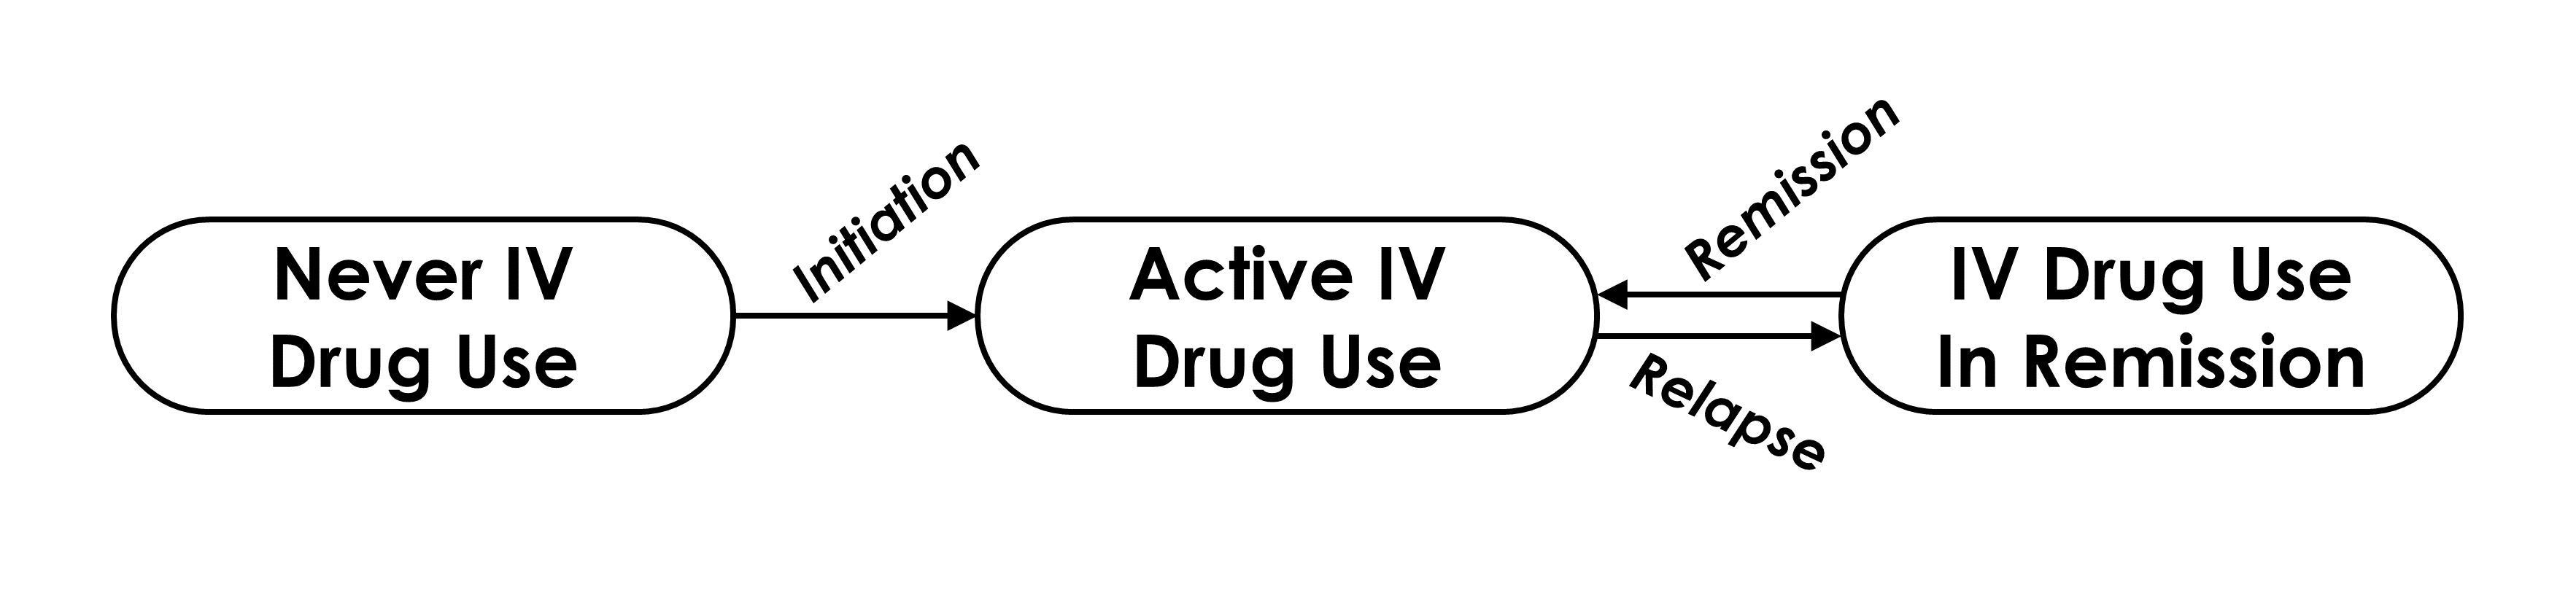
\includegraphics[width=0.75\textwidth]{../base/images/idu_transitions}
	}
\end{figure}

\subsubsection{Time-Varying Parameters}

Many of the parameters in our differential equations are time-varying. We present the differential equations here using general formulations for time-varying parameters (e.g., $\theta(t)$ for mortality rate). In section \ref{functional_forms} - "\nameref{functional_forms}" - we present the specific functional forms we used to allow parameters to vary over time. 


\subsection{HIV Transmission}\label{transmission}

For shorthand, here we will replace $a,r,s,k$ by $i$ and $j$ to index strata of age $\times$ race $\times$ sex/sexual behavior $\times$ IV drug use, where there are $N=A\cdot R \cdot S \cdot K$ total strata ($i,j = 1, ..., N$)
\newline
\newline

The rate of new infections into stratum $i$ at time $t$ - denoted $\Delta_i(t)$ - is the sum of the rates of new infections by each of the $M$ modes of transmission:

\begin{equation}
\Delta_i(t) = \sum_{m=1}^M \Delta_{i,m}(t)
\end{equation}

where $\Delta_{i,m}(t)$ is the rate of new infections into stratum $i$ by transmission mode $m$ at time $t$, which is the sum over all strata $j$ of the rate of new infections into stratum $i$ from contact with stratum $j$ via mode $m$ of transmission:

\begin{equation}
\Delta_{i,m}(t) = \sum_{j=1}^N \Delta_{i,j,m}(t)
\end{equation}

where $\Delta_{i,j,m}(t)$ is the rate of new infections in stratum $i$ due to contact with those infected in stratum $j$ via a mode of transmission $m$ at time $t$. Broadly speaking, this is the product of:

\begin{itemize}
	\item The \textit{transmissibility} from stratum $j$ at time $t$, which is a function of the prevalence of unsuppressed PWH in the stratum.
	\item The proportion of stratum $i$'s partners who come from stratum $j$ (for transmission mode $m$) at time $t$, denoted $\Phi_{i,j,m}(t)$
	\item The rate  of transmission from stratum $j$ to stratum $i$ via mode $m$ at time $t$, denoted $\Gamma_{i,j,m}(t)$
	\item The \textit{susceptibility} of stratum $i$ to infection at time $t$ (in this work, this is a function of PrEP coverage within the stratum)
\end{itemize}

\begin{equation}
\Delta_{i,j,m} = transmissibility_{j,m}(t) \times \Phi_{i,j,m}(t) \times \Gamma_{i,j,m}(t) \times susceptibility_{i,m}(t)
\end{equation}

We describe $transmissibility$ and $susceptibility$ in further detail:

\subsubsection{Transmissibility}

The transmissibility of HIV from stratum $j$ via mode of transmission $m$ at time $t$ is a function of the prevalence of unsuppressed HIV in stratum $j$, allowing for PWH in the acute phase of HIV to transmit more and for those who are diagnosed to reduce transmission behaviors:

\begin{equation}
transmissibility_{j,m}(t) = \frac{\eta \cdot  IA_j(t) + IC_j(t) + \eta \cdot PA_j(t) + PC_j(t) + \eta \cdot \upsilon_j(t) \cdot DA_j(t) \cdot [1 - \rho_j(t)] + \upsilon_j(t) \cdot DC_j(t) \cdot [1 - \rho_j(t)]}{U_j(t) + IA_j(t) + IC_j(t) + PA_j(t) + PC_j(t) + DA_j(t) + DC_j(t)}
\end{equation}

where
\begin{itemize}
	\item $\eta$ is the ratio of transmissibility in the acute phase of HIV relative to the chronic phase
	\item $\rho_j(t)$ is the proportion of diagnosed PWH in stratum $j$ who are virally suppressed at time $t$
	\item $\upsilon_j(t)$ is the degree (relative rate) to which PWH who are aware of their diagnosis reduce their transmission behaviors, on average, relative to PWH who are unaware of their diagnosis
\end{itemize}

\subsubsection{Susceptibility}
\begin{equation}
susceptibility_{i,m}(t) = [1-\pi_i(t)] + \pi_i(t) \times \kappa_{i}
\end{equation}


\begin{itemize}
	\item $\pi_{i}(t)$ is the proportion uninfected individuals at risk for HIV in stratum $i$ at time $t$ who are enrolled in a PrEP program
	\item $\kappa_{i}$ is the relative risk of HIV infection for those on PrEP (relative to no PrEP) in stratum $i$
\end{itemize}


\subsection{Uninfected \big($U_{a,r,s,k}(t)$\big)}
The inflows into each stratum $a,r,s,k$ of uninfected are those entering the model at the youngest age bracket or aging into age stratum $a$ and those moving into IV drug use state $k$. The outflows are those who become infected with HIV, as well as those who die, age out of age stratum $a$, or move out of IV drug use state $k$.
\begin{align*}
	\frac{\partial U_{a,r,s,k}(t)}{\partial t} 
	&= \mathbbm{1}_{a=1} \times \lambda_{r} \times P_r(t) + \mathbbm{1}_{a>1} \times \alpha_{a-1,r,s,k}^U(t) \times U_{a-1,r,s,k}(t) \\
	&+ \mathbbm{1}_{k=active\_use} \times [\zeta_{a,r,s}(t) \times U_{a,r,s,never\_use}(t) + \xi_{a,r,s}(t) \times U_{a,r,s,prior\_use}(t)]\\
	&\qquad + \mathbbm{1}_{k=prior\_use} \times \psi_{a,r,s}(t) \times U_{a,r,s,active\_use}(t)\\
	&- \Delta_{a,r,s,k}(t) \\
	&- \theta^G_{a,r,s,k} \times U_{a,r,s,k}(t) - \mathbbm{1}_{k=active\_use} \times \theta^{IDU} \times U_{a,r,s,k}(t) \\
	&- \alpha_{a,r,s,k}^U(t) \times U_{a,r,s,k}(t) \\
	&- U_{a,r,s,k}(t) \times \big[\mathbbm{1}_{k=never\_use} \times \zeta_{a,r,s}(t) + \mathbbm{1}_{k=active\_use} \times \psi_{a,r,s}(t) + \mathbbm{1}_{k=prior\_use} \times \xi_{a,r,s}(t)\big]
\end{align*}

where
\begin{itemize}
	\item $\mathbbm{1}_{a=1}$ evaluates to 1 if $a$ is the first age bracket and 0 otherwise, and $\mathbbm{1}_{a>1}$ evaluates to 0 if $a$ is the first age bracket and 1 otherwise
	\item $\lambda_(t)$ denotes the birth rate for race $r$ at time $t$
	\item $P_r(t)$ is the total size of all strata where race = $r$ at time $t$. i.e.
		\begin{equation*}
			P_r(t) = \sum_{a,s,k} U_{a,r,s,k}(t) + IA_{a,r,s,k}(t) + IC_{a,r,s,k}(t) + PA_{a,r,s,k}(t) + PC_{a,r,s,k}(t) + DA_{a,r,s,k}(t) + DC_{a,r,s,k}(t)
		\end{equation*}
	\item $\alpha^U_{a-1,r,s,k}$ denotes the aging rate at time $t$ of uninfected individuals in the age stratum before $a$ - the average rate at which uninfected individuals move from age stratum $a-1$ to $a$
	\item $\mathbbm{1}_{k=active\_use}$ evaluates to 1 if $k$ denotes a compartment of active IV drug use and 0 otherwise, and $\mathbbm{1}_{k=prior\_use}$ evaluates to 1 if $k$ denotes a compartment of prior IV drug use
	\item $\zeta_{a,r,s}(t)$ denotes the rate of first-time initiation of IV drug use at time $t$ in stratum $a,r,s$
	\item $\xi_{a,r,s}(t)$ denotes the rate of relapse into IV drug use among prior users of IV drugs at time $t$ in stratum $a,r,s$
	\item $\psi_{a,r,s}(t)$ denotes the rate of remission of IV drug use among active users at time $t$ in stratum $a,r,s$
	\item $U_{a,r,s,never\_use}$, $U_{a,r,s,prior\_use}$, $U_{a,r,s,active\_use}$ denote the compartments with the same age, race, and sex/sexual behavior as $a,r,s,k$ but whose IV drug use stratum is "never use", "prior use", or "active use" respectively	
	\item $\Delta_{a,r,s,k}(t)$ denotes the number of new HIV infections in stratum $a,r,s,k$ at time $t$. This is detailed in Section \ref{transmission} on page \pageref{transmission}
	\item $\theta^G_{a,r,s,k}$ denotes the general mortality rate of individuals in stratum $a,r,s,k$
	\item  $\theta^{IDU}$ denotes the excess mortality rate due to active IV drug use
	\item $\alpha^U_{a,r,s,k}(t)$ denotes the aging rate at time $t$ for uninfected individuals in stratum $a,r,s,k$

\end{itemize}

\subsection{Undiagnosed, Acute HIV \big($IA_{a,r,s,k}(t)$\big)}

The inflows into each stratum $a,r,s,k$ of acute, undiagnosed HIV are the new infections among those who were not on PrEP, those aging into age stratum $a$, and those moving into IV drug use state $k$. The outflows are those who get diagnosed or progress to chronic HIV, as well as those who die (from HIV or other causes), age out of age stratum $a$, or move out of IV drug use state $k$.

\begin{align*}
\frac{\partial IA_{a,r,s,k}(t)}{\partial t} 
&= \Delta_{a,r,s,k}(t) \times [1-\mu_{a,r,s,k}(t)]\\
&+ \mathbbm{1}_{a>1} \times \alpha_{a-1,r,s,k}^H(t) \times IA_{a-1,r,s,k}(t) \\
&+ \mathbbm{1}_{k=active\_use} \times [\zeta_{a,r,s}(t) \times IA_{a,r,s,never\_use}(t) + \xi_{a,r,s}(t) \times IA_{a,r,s,prior\_use}(t)]\\
&\qquad + \mathbbm{1}_{k=prior\_use} \times \psi_{a,r,s}(t) \times IA_{a,r,s,active\_use}(t)\\
&- \beta_{a,r,s,k}(t) \times IA_{a,r,s,k}(t) \\
&- \tau \times IA_{a,r,s,k}(t) \\
&- \theta^{HIV}(t) \times IA_{a,r,s,k}(t)  
- \theta^G_{a,r,s,k} \times IA_{a,r,s,k}(t) 
- \mathbbm{1}_{k=active\_use} \times \theta^{IDU} \times IA_{a,r,s,k}(t) \\
&- \alpha_{a,r,s,k}^H(t) \times IA_{a,r,s,k}(t) \\
&- IA_{a,r,s,k}(t) \times \big[\mathbbm{1}_{k=never\_use} \times \zeta_{a,r,s}(t) + \mathbbm{1}_{k=active\_use} \times \psi_{a,r,s}(t) + \mathbbm{1}_{k=prior\_use} \times \xi_{a,r,s}(t)\big]
\end{align*}


where
\begin{itemize}
	\item $\mu_{a,r,s,k}(t)$ denotes the proportion of new infections in stratum $a,r,s,k$ at time $t$ that were among individuals on PrEP. 
	\begin{equation*}
		\mu_{a,r,s,k}(t) = \frac{\pi_{a,r,s,k}(t) \times \kappa_{a,r,s,k}}{[1-\pi_{a,r,s,k}(t)] + \pi_{a,r,s,k}(t) \times \kappa_{a,r,s,k}}
	\end{equation*} where $\pi_{a,r,s,k}(t)$ is the proportion uninfected individuals at risk for HIV in stratum $a,r,s,k$ at time $t$ who are enrolled in a PrEP program, and $\kappa_{a,r,s,k}$ is the relative risk of HIV infection for PrEP use in stratum $a,r,s,k$
	\item $\alpha_{a-1,r,s,k}^H(t)$ denotes the aging rate of HIV-positive individuals in the age stratum prior to $a$
	\item $\beta_{a,r,s,k}(t)$ is the rate of diagnosis of HIV for those in stratum $a,r,s,k$ at time $t$
	\item $\tau$ is the rate of progression from acute to chronic HIV
	\item $\theta^{HIV}(t)$ is the (time-varying) rate of excess mortality from unsuppressed HIV
	\item $\alpha^H_{a,r,s,k}(t)$ is the aging rate at time $t$ for PWH in stratum $a,r,s,k$
\end{itemize}

\subsection{Undiagnosed, Acute HIV, Enrolled in a PrEP Program \big($PA_{a,r,s,k}(t)$\big)}

The inflows into each stratum $a,r,s,k$ of acute, undiagnosed HIV among those enrolled in a PrEP program are the proportion of new infections among those who were on PrEP, those aging into age stratum $a$, and those moving into IV drug use state $k$. The outflows are those who get diagnosed or progress to chronic HIV, as well as those who die (from HIV or other causes), age out of age stratum $a$, or move out of IV drug use state $k$.

\begin{align*}
\frac{\partial PA_{a,r,s,k}(t)}{\partial t} 
&= \Delta_{a,r,s,k}(t) \times \mu_{a,r,s,k}(t)\\
&+ \mathbbm{1}_{a>1} \times \alpha_{a-1,r,s,k}^H(t) \times PA_{a-1,r,s,k}(t) \\
&+ \mathbbm{1}_{k=active\_use} \times [\zeta_{a,r,s}(t) \times PA_{a,r,s,never\_use}(t) + \xi_{a,r,s}(t) \times PA_{a,r,s,prior\_use}(t)]\\
&\qquad + \mathbbm{1}_{k=prior\_use} \times \psi_{a,r,s}(t) \times PA_{a,r,s,active\_use}(t)\\
&- \beta^{PrEP} \times PA_{a,r,s,k}(t) \\
&- \tau \times PA_{a,r,s,k}(t) \\
&- \theta^{HIV}(t) \times PA_{a,r,s,k}(t)  
- \theta^G_{a,r,s,k} \times PA_{a,r,s,k}(t) 
- \mathbbm{1}_{k=active\_use} \times \theta^{IDU} \times PA_{a,r,s,k}(t) \\
&- \alpha_{a,r,s,k}^H(t) \times PA_{a,r,s,k}(t) \\
&- PA_{a,r,s,k}(t) \times \big[\mathbbm{1}_{k=never\_use} \times \zeta_{a,r,s}(t) + \mathbbm{1}_{k=active\_use} \times \psi_{a,r,s}(t) + \mathbbm{1}_{k=prior\_use} \times \xi_{a,r,s}(t)\big]
\end{align*}

where
\begin{itemize}
	\item $\beta^{PrEP}$ is the rate of diagnosis of HIV among those enrolled in a PrEP program
\end{itemize}

\subsection{Diagnosed, Acute HIV \big($DA_{a,r,s,k}(t)$\big)}

The inflows into each stratum $a,r,s,k$ of acute, diagnosed HIV are new HIV diagnoses among those with undiagnosed, acute HIV (those enrolled in a PrEP program and not), those aging into age stratum $a$, and those moving into IV drug use state $k$. The outflows are those who progress to chronic HIV, as well as those who die (from unsuppressed HIV or other causes), age out of age stratum $a$, or move out of IV drug use state $k$.

\begin{align*}
\frac{\partial DA_{a,r,s,k}(t)}{\partial t} 
&= \beta_{a,r,s,k}(t) \times IA_{a,r,s,k}(t) + \beta^{PrEP} \times PA_{a,r,s,k}(t) \\
&+ \mathbbm{1}_{a>1} \times \alpha_{a-1,r,s,k}^H(t) \times DA_{a-1,r,s,k}(t) \\
&+ \mathbbm{1}_{k=active\_use} \times [\zeta_{a,r,s}(t) \times DA_{a,r,s,never\_use}(t) + \xi_{a,r,s}(t) \times DA_{a,r,s,prior\_use}(t)]\\
&\qquad + \mathbbm{1}_{k=prior\_use} \times \psi_{a,r,s}(t) \times DA_{a,r,s,active\_use}(t)\\
&- \beta_{a,r,s,k}(t) \times DA_{a,r,s,k}(t) \\
&- \tau \times DA_{a,r,s,k}(t) \\
&- \theta^{HIV}(t) \times DA_{a,r,s,k}(t) \times [1-\rho_{a,r,s,k}(t)]
- \theta^G_{a,r,s,k} \times DA_{a,r,s,k}(t) 
- \mathbbm{1}_{k=active\_use} \times \theta^{IDU} \times DA_{a,r,s,k}(t) \\
&- \alpha_{a,r,s,k}^H(t) \times DA_{a,r,s,k}(t) \\
&- DA_{a,r,s,k}(t) \times \big[\mathbbm{1}_{k=never\_use} \times \zeta_{a,r,s}(t) + \mathbbm{1}_{k=active\_use} \times \psi_{a,r,s}(t) + \mathbbm{1}_{k=prior\_use} \times \xi_{a,r,s}(t)\big]
\end{align*}

where
\begin{itemize}
	\item $\rho_{a,r,s,k}(t)$ is the proportion of those with diagnosed HIV in stratum $a,r,s,k$ who are virally suppressed at time $t$.
\end{itemize}

\subsection{Undiagnosed, Chronic HIV \big($IC_{a,r,s,k}(t)$\big)}

The inflows into each stratum $a,r,s,k$ of chronic, undiagnosed HIV are those who progress from acute to chronic HIV, those aging into age stratum $a$, and those moving into IV drug use state $k$. The outflows are those who get diagnosed, as well as those who die (from HIV or other causes), age out of age stratum $a$, or move out of IV drug use state $k$.

\begin{align*}
\frac{\partial IC_{a,r,s,k}(t)}{\partial t} 
&= \tau \times IA_{a,r,s,k}(t) \\
&+ \mathbbm{1}_{a>1} \times \alpha_{a-1,r,s,k}^H(t) \times IC_{a-1,r,s,k}(t) \\
&+ \mathbbm{1}_{k=active\_use} \times [\zeta_{a,r,s}(t) \times IC_{a,r,s,never\_use}(t) + \xi_{a,r,s}(t) \times IC_{a,r,s,prior\_use}(t)]\\
&\qquad + \mathbbm{1}_{k=prior\_use} \times \psi_{a,r,s}(t) \times IC_{a,r,s,active\_use}(t)\\
&- \beta_{a,r,s,k}(t) \times IC_{a,r,s,k}(t) \\
&- \theta^{HIV}(t) \times IC_{a,r,s,k}(t)  
- \theta^G_{a,r,s,k} \times IC_{a,r,s,k}(t) 
- \mathbbm{1}_{k=active\_use} \times \theta^{IDU} \times IC_{a,r,s,k}(t) \\
&- \alpha_{a,r,s,k}^H(t) \times IC_{a,r,s,k}(t) \\
&- IC_{a,r,s,k}(t) \times \big[\mathbbm{1}_{k=never\_use} \times \zeta_{a,r,s}(t) + \mathbbm{1}_{k=active\_use} \times \psi_{a,r,s}(t) + \mathbbm{1}_{k=prior\_use} \times \xi_{a,r,s}(t)\big]
\end{align*}

\subsection{Undiagnosed, Chronic HIV, Enrolled in a PrEP Program \big($PC_{a,r,s,k}(t)$\big)}

The inflows into each stratum $a,r,s,k$ of chronic, undiagnosed HIV among those enrolled in a PrEP program are those who progress from acute to chronic HIV, those aging into age stratum $a$, and those moving into IV drug use state $k$. The outflows are those who get diagnosed, as well as those who die (from HIV or other causes), age out of age stratum $a$, or move out of IV drug use state $k$.
\begin{align*}
\frac{\partial PC_{a,r,s,k}(t)}{\partial t} 
&= \tau \times PA_{a,r,s,k}(t) \\
&+ \mathbbm{1}_{a>1} \times \alpha_{a-1,r,s,k}^H(t) \times PC_{a-1,r,s,k}(t) \\
&+ \mathbbm{1}_{k=active\_use} \times [\zeta_{a,r,s}(t) \times PC_{a,r,s,never\_use}(t) + \xi_{a,r,s}(t) \times PC_{a,r,s,prior\_use}(t)]\\
&\qquad + \mathbbm{1}_{k=prior\_use} \times \psi_{a,r,s}(t) \times PC_{a,r,s,active\_use}(t)\\
&- \beta^{PrEP} \times PC_{a,r,s,k}(t) \\
&- \theta^{HIV}(t) \times PC_{a,r,s,k}(t)  
- \theta^G_{a,r,s,k} \times PC_{a,r,s,k}(t) 
- \mathbbm{1}_{k=active\_use} \times \theta^{IDU} \times PC_{a,r,s,k}(t) \\
&- \alpha_{a,r,s,k}^H(t) \times PC_{a,r,s,k}(t) \\
&- PC_{a,r,s,k}(t) \times \big[\mathbbm{1}_{k=never\_use} \times \zeta_{a,r,s}(t) + \mathbbm{1}_{k=active\_use} \times \psi_{a,r,s}(t) + \mathbbm{1}_{k=prior\_use} \times \xi_{a,r,s}(t)\big]
\end{align*}

\subsection{Diagnosed, Chronic HIV \big($DC_{a,r,s,k}(t)$\big)}

The inflows into each stratum $a,r,s,k$ of chronic, diagnosed HIV are new HIV diagnoses among those with undiagnosed, chronic HIV (those enrolled in a PrEP program and not), those who progress from acute to chronic HIV, those aging into age stratum $a$, and those moving into IV drug use state $k$. The outflows are those who die (from unsuppressed HIV or other causes), age out of age stratum $a$, or move out of IV drug use state $k$.

\begin{align*}
\frac{\partial DC_{a,r,s,k}(t)}{\partial t} 
&= \beta_{a,r,s,k}(t) \times IC_{a,r,s,k}(t) + \beta^{PrEP} \times PC_{a,r,s,k}(t) \\
&+ \tau \times DA_{a,r,s,k}(t) \\
&+ \mathbbm{1}_{a>1} \times \alpha_{a-1,r,s,k}^H(t) \times DC_{a-1,r,s,k}(t) \\
&+ \mathbbm{1}_{k=active\_use} \times [\zeta_{a,r,s}(t) \times DC_{a,r,s,never\_use}(t) + \xi_{a,r,s}(t) \times DC_{a,r,s,prior\_use}(t)]\\
&\qquad + \mathbbm{1}_{k=prior\_use} \times \psi_{a,r,s}(t) \times DC_{a,r,s,active\_use}(t)\\
&- \beta_{a,r,s,k}(t) \times DC_{a,r,s,k}(t) \\
&- \theta^{HIV}(t) \times DC_{a,r,s,k}(t) \times [1-\rho_{a,r,s,k}(t)]
- \theta^G_{a,r,s,k} \times DC_{a,r,s,k}(t) 
- \mathbbm{1}_{k=active\_use} \times \theta^{IDU} \times DC_{a,r,s,k}(t) \\
&- \alpha_{a,r,s,k}^H(t) \times DC_{a,r,s,k}(t) \\
&- DC_{a,r,s,k}(t) \times \big[\mathbbm{1}_{k=never\_use} \times \zeta_{a,r,s}(t) + \mathbbm{1}_{k=active\_use} \times \psi_{a,r,s}(t) + \mathbbm{1}_{k=prior\_use} \times \xi_{a,r,s}(t)\big]
\end{align*}


%---------------------------------%
%-- CALIBRATION METHOD --%
%---------------------------------%

\section{Running And Calibrating the Model}

\subsection{Initializing and Running the Model}

We initialize the model with population sizes from 2007, and seed three HIV cases, one to each race, in the stratum of MSM aged 35-44yo.

We let the model start running at 1970 with this initial state, and run forward to 2007. From 1970 to 2007, we keep the sizes of each stratum of age $\times$ race $\times$ sex/sexual behavior constant; the prevalence of HIV and IV drug use states can vary within these strata. (Fixing strata sizes allowed us to avoid having to replicate birth patterns prior to the 2010-2030 time period).

We continue running the model from 2007 to 2030, without the requirement that strata sizes remain constant.


\subsection{Calibration Method}
To fit our 131 sampled parameters in each MSA, we use Adaptive Metropolis Sampling, a Markov-chain Monte-Carlo technique first described by Haario et. al.\cite{haario2001}. We use a variation of algorithm 5 ("componentwise" sampling) in Andrieu et. al \cite{andrieu2008}, in which we sample blocks of 1 to 6 parameters at a time in a "blockwise" fashion.

For each iteration of the MCMC, we: 
\begin{enumerate}
	\item Sample the new parameters for the block
	\item Run a simulation using the parameters (the new values for parameters in the block, and prior values for parameters not in the block)
	\item Compute the likelihood (and prior for the parameters) and accept or reject
\end{enumerate}

\subsubsection{Finding Initial Parameter Values} \label{init_params}
For each location, we developed a set of starting parameter values by manually calibrating transmission rates and age susceptibilities so that the marginal reported diagnoses and prevalence by age, by race, and by risk factor visually approximated the calibration targets. All other parameter values were left at their "best guess" values (the median for parameters following a Log-normal prior).

Using these starting values, we ran an exploratory, single-chain Adaptive Metropolis Sampling Process for 20,000 iterations with a target acceptance rate of 0.10. We discarded the first 10,000 parameter sets and thinned the remainder to every 20th set, yielding 500 parameter sets. For each parameter value, we calculated a mean and standard deviation on the log scale across the 500 values, as well as correlations with all other parameters. We used the resulting Log-Multivariate-Normal distribution to sample initial parameters for the MCMC runs described below.


\subsubsection{Likelihood and Priors}

In our deterministic, compartmental model, there is a one-to-one correlation between parameters and simulations. The likelihood function can only be computed on a simulation once it has run. Our log-likelihood is actually the sum of ten independent sub-likelihoods, detailed in Section \ref{likelihood}.

The prior distributions for parameters are mostly Log-Normal distributions (a few are Logit-Normal or Uniform), as detailed in Table \ref{params_tab}.

\subsubsection{MCMC Sampling}

For each location, we ran four chains, sampling starting parameter values for each chain from the Log-Multivariate-Normal distribution described above in section \ref{init_params}. For each chain, we ran 50,000 burn-in iterations followed by 50,000 sampling iterations. We thinned to every 200th iteration, leaving us with a set of 1,000 simulations. We used a target acceptance rate of 0.234.

We assessed for convergence using the split-$\hat{r}$ described in Gelman,\cite{gelman2014} as well as visual inspection of trace plots for important or poorly mixing parameters.


%---------------------------------%
%-- LIKELIHOOD --%
%---------------------------------%


\section{The Likelihood} \label{likelihood}

Our likelihood decomposes into 10 independent likelihoods for each of the 10 calibration targets: new diagnoses, prevalence, HIV mortality, proportion of PWH aware of their diagnosis, proportion of PWH virally suppressed, number of at-risk individuals receiving prescriptions for emtricitabine/tenofovir, probability of receiving an HIV test, prevalence of injection drug use, historical AIDS mortality (prior to 2002), and historical reported diagnoses (1998-2002).

\subsection{Calibrating Model Rates to Observed Data: Binomial Likelihood}\label{binomial_likelihood}
In general, for each of our outcome targets, we will use some variation of a binomial likelihood that maps the probability of an outcome in stratum $i$ in a simulation to the number of events in reported data.

\begin{equation}
	y_{i,t} \sim Binomial(n_t, p_{i,t})
\end{equation}

where
\begin{itemize}
	\item $y_{i,t}$ is the reported outcome in subgroup $i$ at time $t$
	\item $n_t$ is the total population size at time $t$
	\item $p_{i,t}$ is the simulated outcomes in subgroup $i$ at time $t$ divided by the simulated total population size at time $t$
\end{itemize}

Note that we scale our outcome probabilities - even for a subgroup - relative to the total population. For example, if we were calibrating to the number of reported diagnoses in MSM in 2015, $p_{i,t}$ would be the simulated number of new infections among MSM in 2015 divided by the \textit{total} simulated population in 2015. Similarly, the $n_t$ used in our likelihood represents the \textit{total} population, even when calibrating a subgroup.

Formulating the likelihood in this way allows us to avoid conditioning on subgroup numbers that are not known or known imperfectly. For example, the true number of MSM is not recorded by the US census. While estimates are available, they are imprecise and not stratified by race.

In actuality, we use the Normal approximation to the binomial, which is computationally more efficient and allows us to formulate multivariate likelihoods easily:
\begin{equation}
	y_{i,t} \sim Normal\Big(n_t \cdot p_{i,t}, n_t \cdot p_{i,t} \cdot (1-p_{i,t}) \Big)
\end{equation}

\subsection{Mapping Outcomes in Stratified Compartments to Reported Marginal Observations}\label{likelihood_mapping}

Our model produces estimates of each outcome in 135 strata per year of age (5 brackets), race (Black, Hispanic, Other), sex/sexual behavior (MSM, heterosexual male, female), and IV drug use (never use, active use, prior use). Calibration targets are rarely reported as fully stratified. To calibrate to marginal data, we use a multivariate likelihood which uses matrix multiplication to aggregate strata into marginal subgroups.

To illustrate, we use a simplified example in which a model partitions the population four strata of age (young vs. old) and sex (male vs. female), but calibrates to marginal outcomes at time $t$: $y_{young,t}$, $y_{old,t}$, $y_{male,t}$, $y_{female,t}$.

We presume that:
\begin{align*}
	y_{young,t} &= y_{young,male,t} + y_{young,female,t}\\
	y_{old,t} &= y_{old,male,t} + y_{old,female,t}\\
	y_{male,t} &= y_{young,male,t} + y_{old,male,t}\\
	y_{female,t} &= y_{young,female,t} + y_{old,female,t}\\
\end{align*}
$y_{young,male,t}$, $y_{young,female,t}$, $y_{old,male,t}$, $y_{old,female,t}$ are not actually reported. However, we formulate the likelihood we would use if they were, using an independent, binomial likelihood for each of the four stratified outcomes:

\begin{align*}
	y_{young,male,t} &\sim Binomial(n_t, p_{young,male,t}) \\
	y_{young,female,t} &\sim Binomial(n_t, p_{young,female,t}) \\
	y_{old,male,t} &\sim Binomial(n_t, p_{old,male,t}) \\
	y_{old,female,t} &\sim Binomial(n_t, p_{old,female,t}) \\
\end{align*}

For computational efficiency and to facilitate multivariate formulation, we use the normal approximation to the binomial:

\begin{align*}
	y_{young,male,t} &\sim Normal\big(n_t \times p_{young,male,t}, n_t \times p_{young,male,t} \times (1-p_{young,male,t})\big) \\
	y_{young,female,t} &\sim Normal\big(n_t \times p_{young,female,t}, n_t \times p_{young,female,t} \times (1-p_{young,female,t})\big) \\
	y_{old,male,t} &\sim Normal\big(n_t \times p_{old,male,t}, n_t \times p_{old,male,t} \times (1-p_{old,male,t})\big) \\
	y_{old,female,t} &\sim Normal\big(n_t \times p_{old,female,t}, n_t \times p_{old,female,t} \times (1-p_{old,female,t})\big) \\
\end{align*}

We write this as a multivariate normal distribution with a mean vector corresponding to the four individual means and a diagonal variance-covariance matrix whose diagonal elements are the four individual variances:

\begin{equation}
	\bm{y_t^\prime} = 
	\begin{bmatrix}
	y_{young,male,t} \\ y_{young,female,t} \\ y_{old,male,t} \\ y_{old,female,t}
	\end{bmatrix} \sim Multivariate\text{-}Normal(\bm{\mu_t}, \bm{\Sigma_t})
\end{equation}

Next, we formulate a matrix, $\bm{M}$, that maps from the unobserved, stratified outcomes to the marginal outcomes which we do observe:

\begin{equation}
	\bm{y_t} = \begin{bmatrix}
		y_{young,t} \\ y_{old,t} \\ y_{male,t} \\ y_{female,t}
	\end{bmatrix} =
	\begin{bmatrix}
	1 & 1 & 0 & 0 \\
	0 & 0 & 1 & 1 \\
	1 & 0 & 1 & 0 \\
	0 & 1 & 0 & 1 \\
	\end{bmatrix}
	\begin{bmatrix}
	y_{young,male,t} \\ y_{young,female,t} \\ y_{old,male,t} \\ y_{old,female,t}
	\end{bmatrix} =
	\bm{M_t} \begin{bmatrix}
	y_{young,male,t} \\ y_{young,female,t} \\ y_{old,male,t} \\ y_{old,female,t}
	\end{bmatrix} =
	\bm{M_t} \bm{y_t^\prime}
\end{equation}

Using this matrix, we can map the likelihood over the unobserved, stratified outcomes to a likelihood over the observed, marginal outcomes:
\begin{equation}
	\bm{y_t} \sim Multivariate\text{-}Normal\big(\bm{M_t \mu_t}, \bm{M \Sigma_t M_t^T}\big)
\end{equation}

This formulation preserves the correlations induced by calibrating to marginal outcomes. For example, if a simulation over-estimated the young, male stratum, we would expect the overestimation of both the total young and overestimation of the total male to be related.

We can extend this approach to formulate a matrix $\bm{M}$ that maps our 135 strata to any set of marginal outcomes. We can map to two-level marginals (e.g., new diagnoses reported by sex and age bracket).

We can also extend this approach across multiple years by assuming that the errors in any one year are independent of other years:

\begin{equation}
	\bm{y} = 
	\begin{bmatrix}
		\bm{y_{t1}} \\
		\bm{y_{t2}} \\
		\vdots \\
		\bm{y_{tT}}
	\end{bmatrix}
	\sim Multivariate\text{-}Normal\big(\bm{M} \bm{\mu}, \bm{M} \bm{\Sigma} \bm{M}^T\big) \label{eq_mapping}
\end{equation}

where
\begin{itemize}
	\item $T$ is the number of years we include
	\item $\bm{\mu} = \begin{bmatrix}
		\bm{\mu_{t1}} \\
		\bm{\mu_{t2}} \\
		\vdots \\
		\bm{\mu_{tT}}
		\end{bmatrix}$
	\item $\bm{M} = \begin{bmatrix}
		\bm{M_{t1}} & \bm{0} & \dots & \bm{0} \\
		\bm{0} & \bm{M_{t2}} & \dots & \bm{0} \\
		\vdots & \vdots & \ddots & \vdots \\
		\bm{0} & \bm{0} & \dots & \bm{M_{tT}}
		\end{bmatrix}$
	\item $\bm{\Sigma} = \begin{bmatrix}
		\bm{\Sigma_{t1}} & \bm{0} & \dots & \bm{0} \\
		\bm{0} & \bm{\Sigma_{t2}} & \dots & \bm{0} \\
		\vdots & \vdots & \ddots & \vdots \\
		\bm{0} & \bm{0} & \dots & \bm{\Sigma_{tT}}
		\end{bmatrix}$
\end{itemize}	



\subsection{Incorporating Measurement Error}\label{measurement_error}

The formulation described in Section \ref{likelihood_mapping} above captures error that stems from the degree to which model simulations depart from reported outcomes. However, we also consider that reported outcomes are imperfect measures of a "true" outcome, and adjust our likelihoods accordingly.
For this formulation, we introduce $y^*_{i,t}$ - the true (unobserved) outcome for subgroup $i$ at time $t$, and use it to decomponse the relationship between $y_{i,t}$ - the reported outcome - and simulated outcomes.

For every subgroup $i$ and time $t$, we write:

\begin{equation}
	y_{i,t} = y^*_{i,t} + Bias_{i,t} + \epsilon_{i,t} \label{eq_reported_to_truth}
\end{equation}

\begin{itemize}
	\item $y_{i,t}$ is the reported (measured) outcome for subgroup $i$ at time $t$ to which we calibrate
	\item $y^*_{i,t}$ is the true (unobserved) outcome 
	\item $Bias_{i,t}$ represents the bias.	We set this term to zero for most reported outcomes. However, some outcomes are expected to differ systematically from the truth. For example, with respect to HIV mortality, it is known that a small proportion of deaths in PWH are not reported to the National Death Index \cite{hanna2009,trepka2011}.
	\item $\epsilon_{i,t}$ The measurement error for outcome $y_{i,t}$
\end{itemize}

We can vectorize Equation \ref{eq_reported_to_truth}
\begin{equation}
	\bm{y} = \bm{y^*} + \bm{Bias} + \bm{\epsilon}
\end{equation}

We let
\begin{equation}
	\bm{Bias} \sim Multivariate\textit{-}Normal\Big(\bm{B}, \bm{\Sigma_B}\Big) \label{eq_bias}
\end{equation}

\begin{equation}
	\bm{\epsilon} \sim Multivariate\textit{-}Normal\Big(\bm{0}, \bm{\Sigma_\epsilon}\Big) \label{eq_epsilon}
\end{equation}

And we replace $\bm{y}$ in Equation \ref{eq_mapping} with $\bm{y^*}$:
\begin{equation}
	\bm{y^*} \sim Multivariate\text{-}Normal\big(\bm{M} \bm{\mu}, \bm{M} \bm{\Sigma} \bm{M}^T\big) \label{eq_mapping_ystar}
\end{equation}

We can combine Equations \ref{eq_bias}, \ref{eq_epsilon}, and \ref{eq_mapping_ystar} to yield a likelihood that incorporates different sources of error: the degree to which the model deviate from the truth, measurement error of reported outcomes, and bias.

\begin{equation}
	\bm{y} \sim Multivariate\textit{-}Normal\Big(\bm{M} \bm{\mu} + \bm{B},
		\bm{M} \bm{\Sigma} \bm{M}^T + \bm{\Sigma_B} + \bm{\Sigma_\epsilon}\Big)
\end{equation}

\subsubsection{Correlated Measurement Errors}\label{correlated_measurement_error}

We also allow for measurement errors and bias to be correlated over time. For example, if estimated prevalent HIV cases among MSM are overestimated in 2015, they are likely to be overestimated in 2016 and 2017 when using the same methods.\cite{fojo2017} To represent these correlations, we decompose $\bm{\Sigma_\epsilon}$ and $\bm{\Sigma_B}$ into a vector of standard deviations, $\bm{\sigma}$ and a correlation matrix, $\bm{\Lambda}$:


\begin{align}
	\bm{\Sigma_\epsilon} &= \bm{\sigma_\epsilon} \bm{\Lambda_\epsilon} \bm{\sigma_\epsilon^T}\\
	\bm{\Sigma_B} &= \bm{\sigma_B} \bm{\Lambda_B} \bm{\sigma_B^T}
\end{align}

In most cases, we give $\bm{\Lambda_\epsilon}$ and $\bm{\Lambda_B}$ a compound symmetry (AKA exchangeable) structure:
\begin{equation}
	\Lambda_{ij} = \begin{cases}
		1 & \text{if } i=j \\
		\rho & \text{if } i \neq j
	\end{cases}
\end{equation}

In general we formulate the standard deviations, $\sigma$ using a coefficient of variance: $\sigma_{i,t} = y_{i,t} \times cv_{i,t}$. We estimate the coefficients of variance and correlation parameters based off of reported data where possible.

%-- Reported Diagnoses --%
\subsection{Reported Diagnoses 2008-2018}

\subsubsection{Calibration Targets}
We calibrate to reported diagnoses from 2008-2018 as reported by the CDC in HIV Atlas\cite{hivatlas} and Metropolitan Statistical Area Reports\cite{msa2010,msa2011,msa2013,msa2014,msa2015,msa2016,cdc24.2}. We fit to total as well as stratified data when available (the years 2010,2011, and 2013-2017):
\begin{itemize}
	\item Total diagnoses for all years 2008-2018
	\item Stratified by age $\times$ sex for 2010, 2011, and 2013-2017
	\item Stratified by race $\times$ sex for 2010, 2011, and 2013-2017
	\item Stratified by risk factor $\times$ sex for 2010, 2011, and 2013-2017
	\item Stratified by race $\times$ risk factor for 2010, 2011, and 2013-2017
\end{itemize}

When the sum of stratified diagnoses from MSA reports did not equal the reported total diagnoses from HIV Atlas, we scaled the stratified diagnoses such that they summed to the total, but maintained the relative proportions of the MSA report.

\subsubsection{Measurement Error}

Because HIV Atlas estimates differed from those in the MSA reports, we were able to estimate the standard deviations of measurement errors by treating the HIV Atlas estimates as truth and the MSA reports as a measured quantity. We formulated the standard deviation as a coefficient of variance multiplied by the estimate, and derived a frequentist maximum likelihood estimate of 0.065 for the coefficient of variance.

Because there was a change in the method of reporting from 2014 to 2015, we assumed that 2008-2014 errors were strongly correlated with a correlation of 0.65, as were 2015-2018 errors, but that errors from the years 2008-2014 had a weaker correlation of 0.25 with errors from 2015-2018.

\subsubsection{Likelihood Formulation}

Using the error terms above, we formulated a multivariate normal likelihood based off of a binomial (Section \ref{binomial_likelihood}) with a mapping to account for correlations between overlapping strata (Section \ref{likelihood_mapping}) and correlated measurement errors (Section \ref{correlated_measurement_error}) using the error terms described above.

\subsubsection{Variance Inflation}
To improve parameter mixing in the MCMC, we inflate the variances for this likelihood by a factor of 4.


%-- Prevalence --%
\subsection{Estimated Prevalence 2008-2018}

\subsubsection{Calibration Targets}
We calibrate to the estimated prevalence (of those aware of their diagnosis) from 2008-2018 as reported by the CDC in HIV Atlas\cite{hivatlas} and Metropolitan Statistical Area Reports\cite{msa2010,msa2011,msa2013,msa2014,msa2015,msa2016,cdc24.2}. We fit to total as well as stratified data when available (the years 2009, 2010, and 2012-2016):
\begin{itemize}
	\item Total diagnoses for all years 2008-2018
	\item Stratified by age $\times$ sex for 2009, 2010, and 2012-2016
	\item Stratified by race $\times$ sex for 2009, 2010, and 2012-2016
	\item Stratified by risk factor $\times$ sex for 2009, 2010, and 2012-2016
	\item Stratified by race $\times$ risk factor for 2009, 2010, and 2012-2016
\end{itemize}

When the sum of stratified prevalence from MSA reports did not equal the reported total prevalence from HIV Atlas, we scaled the stratified prevalences such that they summed to the total, but maintained the relative proportions of the MSA report.

\subsubsection{Measurement Error} \label{prevalence_measurement_error}

As with reported diagnoses, we were able to estimate the standard deviations of measurement errors by treating the HIV Atlas estimates as truth and the MSA reports as a measured quantity. We formulated the standard deviation as a coefficient of variance multiplied by the estimate, and derived a frequentist maximum likelihood estimate of 0.09 for the coefficient of variance.

Because there was a change in the method of reporting from 2014 to 2015, we assumed that 2008-2013 errors were strongly correlated with a correlation of 0.65, as were 2014-2018 errors, but that errors from the years 2008-2013 had a weaker correlation of 0.25 with errors from 2014-2018.

\subsubsection{Likelihood Formulation}

As with reported diagnoses, we formulated a multivariate normal likelihood based off of a binomial (Section \ref{binomial_likelihood}) with a mapping to account for correlations between overlapping strata (Section \ref{likelihood_mapping}) and correlated measurement errors (Section \ref{correlated_measurement_error}) using the error terms described above.

\subsubsection{Variance Inflation}
To improve parameter mixing in the MCMC and to prevent the likelihood for prevalence from dominating the likelihood for reported diagnoses (prevalence has a much larger $p$ than reported diagnoses, so a much smaller binomial variance), we inflate the variances for this likelihood by a factor that is equal to the square-root of the average total prevalence from 2010-2018 divided by the square-root of the average number of reported diagnoses from 2010-2018.

%-- Mortality --%
\subsection{Mortality in PWH 2009-2016}

\subsubsection{Calibration Targets}
We calibrate to the mortality among PWH aware of their diagnosis in 2009, 2010, and 2012-2016 as reported by the CDC in Metropolitan Statistical Area Reports \cite{msa2010,msa2011,msa2013,msa2014,msa2015,msa2016,cdc24.2}. We fit to total mortality as well as mortality stratified by sex.

\subsubsection{Measurement Error}

We took the standard deviation to be a product of the coefficient of variance and the mortality estimate. We used the same coefficient of variance calculated for prevalence (0.09), as well as correlation coefficients (0.65 for 2009-2013 errors with 2009-2013 errors, 0.65 for 2014-2016 errors with 2014-2016 errors, and 0.25 for 2009-2013 errors with 2014-2016 errors).

\subsubsection{Bias}

Because a small proportion of deaths in PWH are not captured by the National Death Index \cite{hanna2009,trepka2011}, we presumed that mortality was biased down by 2.6\% with a standard deviation of 1.3\%.\cite{hanna2009,trepka2011}

\subsubsection{Likelihood Formulation}

We formulate a multivariate normal likelihood analagous to the likelihood for reported diagnoses and mortality, with the addition of the bias term as outlined in Section \ref{measurement_error}.

\subsubsection{Variance Inflation}
To improve parameter mixing in the MCMC, we inflate the variances for this likelihood by a factor of 2.



%-- Awareness of Diagnosis --%
\subsection{Awareness of Diagnosis Among PWH 2010-2018}\label{likelihood_awareness}

\subsubsection{Calibration Targets}
We calibrate to the proportion of PWH who are aware of their disease. For five MSAs (Houston-The Woodlands-Sugar Land, TX; Los Angeles-Long Beach-Anaheim, CA; Memphis, TN-MS-AR; New York-Newark-Jersey City, NY-NJ-PA; Seattle-Tacoma-Bellevue, WA) estimates of the proportion aware for at least 3 years from 2010-2018 were publicly available from local public health websites. For the remaining 27 MSAs, we used the state-level estimates of proportion aware of their diagnoses available through HIV Atlas \cite{hivatlas}. For MSAs that spanned multiple states, we calibrated to the weighted average of the proportion aware, where weights were the population within in the MSA that falls into each state from 2010-2018.

\subsubsection{Formulation of Binomial Likelihood Component}

For each year $t$, we postulated that:
\begin{equation}
	y_t \sim Binomial(\frac{y_t}{\pi_t}, p_t)
\end{equation}

where:
\begin{itemize}
	\item $y_t$ is the prevalence of PWH aware of their diagnosis in year $t$ as reported by the CDC
	\item $\pi_t$ represents our calibration target, the proportion of PWH aware of their diagnosis in year $t$ as reported by the CDC or local health department
	\item $\frac{y_t}{\pi_t}$ is the estimated number of all PWH (both those aware and unaware of their diagnosis) in year $t$
	\item $p_t$ is the simulated proportion of PWH aware of their diagnosis in year $t$
\end{itemize}

In order to generalize to a multivariate likelihood, we used the normal approximation to the binomial:

\begin{equation}
	y_t \sim Normal\Big(\frac{y_t}{\pi_t} \cdot p_t, \frac{x_t}{\pi_t} \cdot p_t \cdot (1 - p_t)\Big)
\end{equation}

\subsubsection{Measurement Error}

We included a measurement error as described in section \ref{correlated_measurement_error}. We assumed that the reported proportion of PWH aware of their diagnosis had a standard deviation of 0.005 when based on county- or MSA-level data data, and a standard deviation of 0.015 when based on state-level data.

We furthermore presumed that measurement errors were correlated across time, using a compound symmetry correlation structure with $\rho = 0.5$

\subsubsection{Likelihood Formulation}
We incorporated the Binomial component and measurement error into a multivariate normal likelihood as described in \ref{likelihood_mapping}.

\subsubsection{Variance Inflation}
To improve parameter mixing in the MCMC, we inflate the variances for this likelihood by a factor of 8.

%-- Viral Suppression --%
\subsection{Viral Suppression Among PWH 2010-2018}\label{likelihood_suppression}

The likelihood for suppression had two independent components: a multivariate-normal component targeting the reported proportion of PWH who were suppressed, and a Bernoulli component to weight whether suppression was increasing or decreasing.

\subsubsection{Calibration Targets}
We calibrated to the proportion of PWH who were suppressed, as reported on local health department websites, for all years between 2010 and 2018 where data were available. If multiple jurisdictions within an MSA reported proportions, we took the weighted average. If no data was available at the county- or MSA-level we used state-level proportions. A total proportion suppressed was available for all 32 MSAs; we also included estimates stratified by age, by race, by sex, and by HIV-acquisition risk factor if they were available.

\subsubsection{Binomial Likelihood Component}

We formulated a multivariate-normal approximation to a Binomial likelihood, similar to the one detailed in Section \ref{binomial_likelihood} with the exceptions that (1) the response was the CDC-reported prevalence of HIV multiplied by the reported proportion suppressed and (2) that the $n$ was the simulated prevalence of diagnosed HIV instead of the total population. We used the matrix mapping described in Section \ref{likelihood_mapping} to account for correlations in overlapping stratifications.

\subsubsection{Measurement Error}
We included a measurement error as described in section \ref{correlated_measurement_error}. We assumed that the reported proportion of PWH aware of their diagnosis had a standard deviation of 0.01 when based on county- or MSA-level data data, and a standard deviation of 0.03 when based on state-level data.

We furthermore presumed that measurement errors were correlated across time, using a compound symmetry correlation structure with $\rho = 0.5$

\subsubsection{Multivariate Normal Likelihood Formulation}
We incorporated the Binomial component and measurement error into a multivariate normal likelihood as described in \ref{likelihood_mapping}.

\subsubsection{Bernoulli Likelihood for Increasing vs. Decreasing Suppression}
In general, suppression is increasing or stable over time in most locations across most subgroups. In order to discourage solutions where one race or age subgroup had decreasing suppression over time but total suppression followed overall trends (which was possible in locations where stratified data on suppression were unavailable), we also included a Bernoulli likelihood. This likelihood specified that the probability that, for each stratum of age, race, sex, and IV drug use, the probability that simulated suppression had a decreasing slope on the logit scale was 0.05 (which we estimated from the average number of reported suppressed proportions that decreased from one year to the next in all locations and all stratifications for which we had data). ie:

\begin{equation}
	\prod_{a,r,s,k} 0.05^{\text{suppression in stratum } a,r,s,k \text{ is decreasing}} \times 0.95^{\text{suppression in stratum } a,r,s,k \text{ is not decreasing}}
\end{equation}




%-- PrEP --%
\subsection{Pharmacy Fills of Prescriptions for PrEP 2012-2018}\label{likelihood_prep}

\subsubsection{Calibration Targets}
We calibrated to the number of prescriptions for Emtricitabine/Tenofovir for use as PrEP from 2012 to 2018, as reported by AIDSVu \cite{aidsvu_prep}. We used both total numbers as well as numbers stratified by age and by sex (although, due to data suppression rules, stratified estimates were sometimes missing).

\subsubsection{Differences between Model Representation and Reported Data}
The concept of PrEP in our model differs from the data reported by AIDSVu in a number of ways, and our likelihood has to make adjustments for these discrepancies.

Our model simulations produce a proportion of at-risk individuals who are currently enrolled in a PrEP program (since most prescriptions for PrEP are written on a 3-month basis, we take this to correspond to a prescription in the past 3 months).

The AIDSVu data report the number of individuals who filled at least one prescription for emtricitabine/tenofovir in the past year, and who were not using it (as judged by a validated algorithm \cite{maccannell2015}) for treatment of HIV infection or viral hepatitis. Pharmacy records come from a commercial dataset that captures 83\% of prescriptions nationally. \cite{sullivan2018}

This introduces several discrepancies:
\begin{enumerate}
	\item Not all individuals who have a prescription for PrEP will be captured in the dataset
	\item Some individuals who take emtricitabine/tenofovir for indications other than PrEP (HIV treatment, viral hepatitis) will be incorrectly classified as taking it for PrEP
	\item Not all individuals who filled a PrEP prescription in the past year will have filled in the past 3 months (ie, have an "active" prescription)
\end{enumerate}

\subsubsection{Adjusting the Calibration Target to Account for Discrepancies}

We mapped our model output to the calibration target - the number of pharmacy fills for emtricitabine/tenofovir - using four adjustment factors, as follows:

\begin{equation}
	y^\prime_i = y_i \times \frac{\pi \cdot \phi \cdot \rho}{\theta}
\end{equation}

where:
\begin{itemize}
	\item $y_{i,t}$ Represents the reported number of pharmacy fills in the past year for a stratum $i$ at time t $t$
	\item $y^\prime_{i,t}$ Represents our adjusted response - the number of individuals on PrEP at time $t$
	\item $\pi$ denotes the proportion of emtricitabine/tenofovir prescriptions classified as for PrEP that are truly for PrEP and not some other indication (the positive predictive value of the algorithm)
	\item $\rho$ denotes the ratio of the number of people with a pharmacy fill in the past three months to the number of people with a pharmacy fill in the past year
	\item $\theta$ denotes the proportion of pharmacy fills that are captured in the dataset
\end{itemize}

As each of the four adjustment factors is itself uncertain, we represented each with a Lognormal distribution:

\begin{align*}
	Ln(\pi)& \sim Normal(\pi^\prime_0, \sigma^{\prime 2}_\pi) \\
	Ln(\rho)& \sim Normal(\rho^\prime_0, \sigma^{\prime 2}_\rho) \\
	Ln(\theta)& \sim Normal(\theta^\prime_0, \sigma^{\prime 2}_\theta) \\
\end{align*}

We derived estimates of the mean and variance for each of the factors from the literature (Table \ref{prep_factors} below). We converted these to the mean and distribution of a Lognormal distribution using the approximation that the log-sd is approximately equation to the coefficient of variance:

\begin{align*}
	\pi^\prime_0 &= Ln(\pi_0) \\
	\sigma^{\prime}_\pi &= \frac{\sigma_\pi}{\pi_0}
\end{align*}

where $\pi_0$ is the mean and $\sigma_\pi$ is the standard deviation for $\pi$ (NOT on the log scale), with analagous calculations for $\rho$ and $\theta$.

This formulation allowed us to articulate a Lognormal distribution for $y^\prime_{i,t}$ - the number of people on PrEP at time $t$ - that is a function of our reported calibration target - $y_{i,t}$ - and the adjustment factors:

\begin{align}
	Ln(y^\prime_{i,t}) &= Ln(y_{i,t}) + Ln(\pi) + Ln(\phi) + Ln(\rho) - Ln(\theta) \\
	&\sim Normal \Big( Ln(y_{i,t}) + \pi^\prime_0 + \rho^\prime_0 - \theta^\prime_0,  \sigma^{\prime 2}_\pi + \sigma^{\prime 2}_\rho + \sigma^{\prime 2}_\theta \Big)
\end{align} 

We used approximations to give $y^\prime_{i,t}$ a Normal distribution that will allow us to more easily fold it into a multivariate likelihood, with mean and variance:

\begin{align*}
	E \big[y^\prime_{i,t} \big] &= y_{i,t} \times \frac{\pi \cdot \rho}{\theta} \\
	Var \big[y^\prime_{i,t} \big] &= \big( \sigma^{\prime 2}_\pi + \sigma^{\prime 2}_\rho + \sigma^{\prime 2}_\theta \big) \times E \big[y^\prime_{i,t} \big] \\
\end{align*}

We imposed a correlation in the effects of these factors across time, by defining the vector $\bm{y^\prime_i}$ of all $y^\prime{i,t}$ to have a compound symmetry matrix with correlation coefficient of 0.5.

\begin{table}[h!]
		\caption{Means and Standard Deviations of PrEP Likelihood Adjustment Factors}
		\label{prep_factors}
		\begin{tabular}{r|c|c|l} 
			\textbf{Adjustment Factor} & \textbf{Mean} & \textbf{Standard Deviation} & \textbf{Reference}\\
			\hline
			Proportion of prescriptions correctly classified as PrEP ($\mathbf{\pi}$) & 0.901 & 0.035 & MacCannell 2015 \cite{maccannell2015} \\
			\hline
			Ratio of PrEP within 3mo to PrEP within 1yr ($\mathbf{\rho}$) & 0.523 & 0.038 & Siegler 2018 \cite{siegler2018}, AIDSVu \cite{aidsvu_prep} \\
			\hline
			Proportion of pharmacy fills captured in dataset ($\mathbf{\theta}$) & 0.83 & 0.05 & Sullivan 2018\cite{sullivan2018} \\
		\end{tabular}
\end{table}

\subsubsection{Measurement Error}
On top of the adjustments mapping pharmacy fills to enrollment in a PrEP program, we allowed for the reported pharmacy fills to have a measurement error standard deviation equal to $\sqrt{y_{i,t}}$. This is based on the assumption that the observed number of pharmacy fills follows a binomial distribution, and when $p$ is small, the variance of a binomial distribution $n \cdot p \cdot (1-p) \approx n \cdot p$.

\subsubsection{Adjusting the probability of taking PrEP to Account for who is 'At-Risk' for HIV}

We postulated that the number of people on PrEP, $y^\prime_{i,t}$, followed a binomial distribution. We took the whole population to be the $n$ of the binomial, which required that the $p$ be the probability of being at risk for HIV AND being on PrEP.

Our model simulations output a probability of being on PrEP for those at risk for acquiring HIV. We multiplied this probability by the probability of being at risk for acquiring HIV to get the overall $p$ for the binomial distribution.

We estimated the proportion at risk for acquiring HIV by calculating the proportion of MSM, PWID, and heterosexuals who meet CDC criteria for PrEP\cite{cdc_prep_guidelines} for each stratum of age and race from NHBS surveillance reports (Tables \ref{prep_indications_msm}, \ref{prep_indications_idu}, \ref{prep_indications_heterosexual}).\cite{nhbs24, nhbs22, nhbs19}. For MSM and heterosexuals, we multiplied this by the proportion in each age bracket who are sexually active (Table \ref{sexual_activity_by_age}).

We used the normal approximation to the binomial to formulate these as a multivariate normal, as described in Section \ref{likelihood_mapping}. Because the proportion indicated for PrEP in a location is likely correlated from year to year, we imposed an autoregressive correlation structure on the distribution with a $\rho=0.9$.

\begin{table}[h!]
		\caption{Estimated Proportion of Sexually Active MSM with Indication for PrEP*}
		\label{prep_indications_msm}
		\begin{tabular}{r|c c c} 
			 & \textbf{Black} & \textbf{Hispanic} & \textbf{Other} \\
			\hline
			\textbf{13-24 years} & 0.363 & 0.416 & 0.476 \\
			\textbf{25-34 years} & 0.429 & 0.492 & 0.562 \\
			\textbf{35-44 years} & 0.420 & 0.482 & 0.551 \\
			\textbf{45-54 years} & 0.370 & 0.424 & 0.485 \\
			\textbf{55+ years} & 0.305 & 0.350 & 0.401 \\
		\end{tabular}
	\begin{flushleft}
	\footnotesize{*Estimated as the proportion reporting condomless sex with a casual partner from the 2017 NHBS Report \cite{nhbs22}}
\end{flushleft}
\end{table}

\begin{table}[h!]
		\caption{Estimated Proportion of PWID with Indication for PrEP*}
		\label{prep_indications_idu}
		\begin{tabular}{r|c c c} 
		 & \textbf{Black} & \textbf{Hispanic} & \textbf{Other} \\
			\hline
			\textbf{13-24 years} & 0.606 & 0.703 & 0.831 \\
			\textbf{25-34 years} & 0.593 & 0.689 & 0.814 \\
			\textbf{35-44 years} & 0.566 & 0.656 & 0.776 \\
			\textbf{45-54 years} & 0.502 & 0.582 & 0.688 \\
			\textbf{55+ years} & 0.419 & 0.486 & 0.575 \\
		\end{tabular}
	\begin{flushleft}
	\footnotesize{*Estimated as the proportion reporting needle-sharing from the 2018 NHBS Report \cite{nhbs24}}
\end{flushleft}
\end{table}

\begin{table}[h!]
		\caption{Estimated Proportion of Heterosexuals with Indication for PrEP*}
		\label{prep_indications_heterosexual}
		\begin{tabular}{r|c c c} 
			 & \textbf{Black} & \textbf{Hispanic} & \textbf{Other} \\
			\hline
			\textbf{13-24 years} & 0.1305 & 0.0611 & 0.0595 \\
			\textbf{25-34 years} & 0.1225 & 0.0574 & 0.0558 \\
			\textbf{35-44 years} & 0.0641 & 0.0300 & 0.0292 \\
			\textbf{45-54 years} & 0.0538 & 0.0252 & 0.0245 \\
			\textbf{55+ years} & 0.0435 & 0.0204 & 0.0198 \\
		\end{tabular}
	\begin{flushleft}
	\footnotesize{*Estimated as the proportion reporting a recent STI in the 2016 NHBS Report \cite{nhbs19}}
\end{flushleft}
\end{table}

\begin{table}[h!]
		\caption{Estimated Proportion of Individuals Who Are Sexually Active, by Age and Race}
		\label{sexual_activity_by_age}
		\begin{tabular}{r|c c} 
			 & \textbf{Female} & \textbf{Male} \\
			\hline
			\textbf{13-24 years} & 0.659 & 0.626 \\
			\textbf{25-34 years} & 0.975 & 0.953 \\
			\textbf{35-44 years} & 0.986 & 0.977 \\
			\textbf{45-54 years} & 0.987 & 0.982 \\
			\textbf{55+ years} & 0.390 & 0.656 \\
		\end{tabular}
	\begin{flushleft}
		\footnotesize{Proportions for 13-54 year olds derived from Mosher 2005 \cite{mosher2005}, for 55+ from Lindau 2007 \cite{lindau2007}}
	\end{flushleft}
\end{table}

\subsubsection{Likelihood Formulation}
We combined these three elements - a multivariate normal deriving from the adjustment factors, a multivariate normal encapsulating the measurement errors, and a multivariate normal approximation of the binomial by adding the mean vectors and covariance matrices.

\subsubsection{Variance Inflation}
To improve parameter mixing in the MCMC, we inflated the variances for this likelihood by a factor of 2.

%-- Testing --%
\subsection{Receipt of HIV Test 2013-2017}\label{likelihood_testing}

\subsubsection{Calibration Targets}
We calibrated testing rates to several targets:
\begin{enumerate}
	\item The total proportion of individuals reporting ever taking an HIV test in the MSA in 2013, 2014, 2016, and 2017, as reported by the Behavioral Risk Factor Surveillance System (BRFSS)\cite{brfss.13.17}
	\item The relative likelihood (odds ratio) by race/ethnicity of reporting ever receiving a test at the state level for Black vs. Non-Black/Non-Hispanic and Hispanic vs. Non-Black/Non-Hispanic as reported by BRFSS.
	\item The relative likelihood (odds ratio) by sex of reporting ever receiving a test at the state level (female vs. male) as reported by BRFSS.
	\item The relative likelihood (odds ratio) by age of reporting ever receiving a test at the state level for 13-24 vs 35-44 years, 25-34 vs 35-44 years, 45-54 vs 35-44 years, and 55+ vs 35-44 years as reported by BRFSS.
\end{enumerate}

We presumed each of these targets to follow an independent likelihood, which we combined

\subsubsection{Likelihood Component for Total Proportion Ever Tested}
The portion of the likelihood which calibrated to the total proportion of individuals reporting ever taking an HIV test incorporated three sources of uncertainty:

\begin{enumerate}
	\item The uncertainty in relating our simulated parameter - the rate of testing in subgroups - to a proportion ever tested
	\item A binomial component which captures the uncertainty in mapping from model simulations to observed calibration targets
	\item Measurement error in the observed calibration targets
\end{enumerate}  

We describe these three components in the next three paragraphs.

\subsubsection{Mapping Model Testing Rates to Proportion Ever Tested} \label{mapping_testing}

Our model simulations produce rates of testing for each compartment, which we needed to map to the probability of ever receiving an HIV test.

We first translated the testing rate for stratum $i$ at time $t$, $r_{i,t}$, to the probability of receiving a test in the past year, $p_{i,t}$, under the assumption that testing follows a Poisson process:

\begin{equation} \label{p_to_rate}
	p_{i,t} = 1 - e^{-r_{i,t}}
\end{equation}


We related the probability of receiving a test in the past year to the probability of ever receiving a test under the following model:

\begin{equation} \label{p_to_p_ever}
	Ln(1-p^{ever}_{i,t}) = \sim Normal\big(\beta \cdot Ln(1-p_{i,t}), \sigma^2\big)
\end{equation}

which postulates that the log-probability of never receiving a test is proportional to the log probability of not receiving at test in the past year. We fit this model using data from NHBS surveys from 2011-2018 \cite{nhbs8,nhbs11,nhbs13,nhbs15,nhbs18,nhbs19,nhbs22,nhbs24}, which reported both the proportion ever receiving a test and the proportion receiving a test in the past year in 23 US metropolitan statistical areas, yielding $\beta = 2.49$, $\sigma=0.046$.

Combining equations \ref{p_to_rate} and \ref{p_to_p_ever} yields:
\begin{equation}
	Ln\big(1 - p^{ever}_{i,t}\big) \sim Normal\big(\beta \cdot r_{i,t}, \sigma^{\prime 2}\big)
\end{equation}

By the properties of the log-normal distribution, we have 
\begin{align} \label{mapping_testing_mu}
	E\big[1-p^{ever}_{i,t}\big] &= \mu_{i,t} = e^{\beta r_{i,t} \cdot \frac{\sigma^{\prime  2}}{2}} \\
	Var\big(1-p^{ever}_{i,t}\big) &= \sigma^2_{i,t} = \big(e^{\sigma^{\prime 2}} - 1) \cdot e^{2 \beta r_{i,t} + \sigma^{\prime 2}}
\end{align}
For feasibility integrating with other components in the likelihood, we approximated this Log-normal for $1-p^{ever}_i$ distribution by a Normal distribution:
\begin{align}
	1 - p^{ever}_{i,t} &\sim Normal\big(\mu_{i,t}, \sigma^2_{i,t}\big) \\
	p^{ever}_{i,t} &\sim Normal\big(1-\mu_{i,t}, \sigma^2_{i,t}\big)
\end{align}

\subsubsection{Binomial Likelihood Component for Total Proportion Ever Tested}

We defined $\hat{p}_{i,t}$ to be the 'true' proportion of individuals in stratum $i$ ever tested for HIV at time $t$, and formulated a binomial likelihood in terms of $p^{ever}_{i,t}$:

\begin{equation}
	n_{i,t} \cdot \hat{p}_{i,t} | p^{ever}_{i,t} \sim Binomial\big(n_{i,t}, p^{ever}_{i,t}\big)
\end{equation}

Where $n_{i,t}$ is the simulated size of stratum $i$ at time $t$.

Using a normal approximation to the binomial gives us:
\begin{equation}
	n_{i,t} \cdot \hat{p}_{i,t} \sim Normal\big(n_{i,t} \cdot p^{ever}_{i,t}, n_{i,t} \cdot p^{ever}_{i,t} \cdot(1-p^{ever}_{i,t} )\big)
\end{equation}

To correspond to the observed total proportion ever tested, we summed across strata:

\begin{align}
	n_t \cdot \hat{p}_t = \sum_i n_{i,t} \cdot \hat{p}_{i,t} &\sim Normal \Big(\sum_i n_{i,t} \cdot p^{ever}_{i,t}, \sum_i n_{i,t} \cdot p^{ever}_{i,t} \cdot(1-p^{ever}_{i,t}) \Big) \\
	\hat{p}_t &\sim Normal \Bigg(\frac{\sum_i n_{i,t} \cdot p^{ever}_{i,t}}{n_t}, \frac{\sum_i n_{i,t} \cdot p^{ever}_{i,t} \cdot(1-p^{ever}_{i,t})}{n_t^2} \Bigg) \\
\end{align}

where $n_t = \sum_i n_{i,t}$

\subsubsection{Measurement Error for Total Proportion Ever Tested}

We calibrated to the reported proportion ever tested for HIV at a given time $t$ for each MSA, which we denote $p^{obs}_t$.

We postulated that this is a noisy measurement of the true proportion ever tested, $\hat{p}_t$:

\begin{equation}
	p^{obs}_t | \hat{p}_t \sim Normal(\hat{p}_t, \tau^2)
\end{equation}

Where $\tau^2$ comes from the Wald interval for the sample data, ie:
\begin{equation}
	\tau^2 = n^{obs}_t \cdot p^{obs}_t \cdot (1-p^{obs}_t)
\end{equation}

We vectorized the observed probabilities, and allowed the measurement errors to be correlated across the resulting multivariate normal distribution:
\begin{equation}
	\bm{p^{obs}} \sim Multivariate\text{-}Normal\big(\bm{\hat{p}}, \bm{\tau} \bm{\Gamma} \bm{\tau}^T \big)
\end{equation}
Where $\bm{\Gamma}$ is a compound symmetry (exchangeable) correlation matrix with $\rho = 0.5$

\subsubsection{Likelihood Components for Odds Ratios of Ever-Testing by Sex, Age, and Race}
We included three likelihood components for the odds ratios of ever receiving a test by sex, age, and race at the state level. These include two sources of uncertainty: measurement error for the reported proportion ever tested, and a binomial error mapping the simulated outputs to observed data.

\subsubsection{Binomial Component for Odds Ratios}

In general, we wanted to compare the proportion ever receiving an HIV test in two subgroups (which we denote 1 and 2) at time $t$.

We defined $\bar{p}_{1,t}$ to be the estimated proportion ever tested in subgroup 1 and $\bar{p}_{2,t}$ to be the estimated proportion ever tested in subgroup 2 at time $t$, and assigned them a binomial distribution:

\begin{align}
	\bar{p}_{1,t} \cdot n_{1,t} &\sim Binomial(n_{1,t}, \bar{\mu}_{1,t}) \\
	\bar{p}_{2,t} \cdot n_{2,t} &\sim Binomial(n_{2,t}, \bar{\mu}_{2,t}) \\
\end{align}

Where we formulated $\bar{\mu}_{1,t}$ and $\bar{\mu}_{2,t}$ using the quantity $\mu_{i,t}$ defined in Section \ref{mapping_testing}, equation \ref{mapping_testing_mu}, 

\begin{align}
\bar{\mu}_{1,t} &= 1 - \frac{\sum_i \mu_{i,t} \cdot n_{i,t} \cdot \mathbbm{1}_{i \in \text{subgroup }1}}{\sum_i n_i \cdot \mathbbm{1}_{i \in \text{subgroup }1}}\\
\bar{\mu}_{2,t} &= 1 - \frac{\sum_i \mu_{i,t} \cdot n_{i,t} \cdot \mathbbm{1}_{i \in \text{subgroup }2}}{\sum_i n_i \cdot \mathbbm{1}_{i \in \text{subgroup }2}}
\end{align}

Using the normal approximation to tbe binomial gives us:
\begin{align}
	\bar{p}_{1,t} \cdot n_{1,t} &\sim Normal\Big(n_{1,t} \cdot \bar{\mu}_{1,t}, n_{1,t} \cdot \bar{\mu}_{1,t} \cdot (1-\bar{\mu}_{1,t})\Big)\\
	\bar{p}_{1,t} &\sim Normal\Bigg(\bar{\mu}_{1,t}, \frac{\bar{\mu}_{1,t} \cdot (1-\bar{\mu}_{1,t})}{n_{1,t}}\Bigg)\\
	\bar{p}_{2,t} &\sim Normal\Bigg(\bar{\mu}_{2,t}, \frac{\bar{\mu}_{2,t} \cdot (1-\bar{\mu}_{2,t})}{n_{2,t}}\Bigg)\\
\end{align}

We used the delta method to derive a distribution for the log odds ratio:

\begin{equation}
	Ln\big(\bar{OR}_{12,t}\big) = Ln\bigg(\frac{\bar{p}_{1,t}}{1-\bar{p}_{1,t}} \cdot {\frac{1 - \bar{p}_{2,t}}{\bar{p}_{2,t}}}\bigg) \sim Normal\Bigg(Ln\bigg(\frac{\bar{\mu}_{1,t}}{1-\bar{\mu}_{1,t}} \cdot {\frac{1 - \bar{\mu}_{2,t}}{\bar{\mu}_{2,t}}}\bigg), \gamma_{12,t}^2\Bigg)
\end{equation}

where 

\begin{equation}
	\gamma_{12,t}^2 = \frac{\bar{\mu}_{1,t} \cdot (1-\bar{\mu}_{1,t})}{n_{1,t}} \times \bigg(\frac{1}{\bar{\mu}_{1,t}} - \frac{1}{1-\bar{\mu}_{1,t}} \bigg)^2 + \frac{\bar{\mu}_{2,t} \cdot (1-\bar{\mu}_{2,t})}{n_{2,t}} \times \bigg(\frac{1}{\bar{\mu}_{2,t}} - \frac{1}{1-\bar{\mu}_{2,t}} \bigg)^2
\end{equation}

\subsubsection{Measurement Error for Odds Ratios}

We defined our response, $OR_{12,t}$, as the odds ratio of the reported proportions ever tested in subgroups 1 and 2 at time $t$ (denoted $p^{obs}_{1,t}$ and $p^{obs}_{2,t}$):


We gave the log odds ratio derived from $\bar{p}_{1,t}$ and $\bar{p}_{2,t}$ a normal distribution centered at $\bar{OR}_{12,t}$ as defined above:

\begin{equation}
	Ln\big(OR_{12,t}\big) \sim Normal\big(\bar{OR}_{12,t}, \sigma_{12,t}^2 \big)
\end{equation}

$\sigma_{12,t}$ is the standard deviation of the log odds ratio calculated from the sample:

\begin{equation}
	\sigma_{12,t} = \sqrt{\frac{1}{p^{obs}_{1,t} \cdot n^{obs}_{1,t}} + \frac{1}{(1-p^{obs}_{1,t}) \cdot n^{obs}_{1,t}} + \frac{1}{p^{obs}_{2,t} \cdot n^{obs}_{2,t}} + \frac{1}{(1-p^{obs}_{2,t}) \cdot n^{obs}_{1,t}}}
\end{equation}

We allowed measurement errors to be correlated over time by vectorizing, and using a multivariate-normal distribution:

\begin{equation}
	\bm{Ln\big(OR_{12}\big)} \sim Multivariate\text{-}Normal\big(\bm{\bar{OR}_{12}}, \bm{\sigma_{12,t}} \bm{\Gamma} \bm{\sigma_{12,t}}^T \big)
\end{equation}

where $\Gamma$ is a compound symmetry correlation matrix with $\rho=0.5$.

\subsubsection{Variance Inflation}
To improve parameter mixing in the MCMC, we inflate the variances for this likelihood by a factor of 64.


%-- IDU --%
\subsection{Injection Drug Use 2014-2016}

\subsubsection{Calibration Targets}
We calibrated simulated IV drug use to four targets each for active use and prior use, drawn from the NSDUH 2014-2016\cite{nsduh}:
\begin{enumerate}
	\item The total prevalence of active IV drug use, calculated as the NSDUH substate estimate for heroin use in the past year multiplied by the national ratio of use of any injection drug within 30 days to use of heroin within the past year
	\item The total prevalence of prior IV drug use, calculated as the NSDUH substate estimate for heroin use in the past year multiplied by the national ratio of use of any injection drug more than 30 days prior to use of heroin within the past year
	\item The odds ratio of the prevalence of drug use within 30 days for Black vs. non-Black/non-Hispanic and non-Black/non-Hispanic, based on national NSDUH surveys
	\item The odds ratio of the prevalence of drug use more than 30 days prior for Black vs. non-Black/non-Hispanic and non-Black/non-Hispanic, based on national NSDUH surveys
	\item The odds ratio of the prevalence of drug use within 30 days for female vs. heterosexual male and MSM vs. heterosexual male, based on national NSDUH surveys
	\item The odds ratio of the prevalence of drug use more than 30 days prior for female vs. heterosexual male and MSM vs. heterosexual male, based on national NSDUH surveys
	\item The odds ratio of the prevalence of drug use within 30 days for 13-24yo vs. 35-44yo, 25-34yo vs 35-44yo, 45-54yo vs 35-44yo, and 55+yo vs. 35-44yo, based on national NSDUH surveys
	\item The odds ratio of the prevalence of drug use more than 30 days prior for 13-24yo vs. 35-44yo, 25-34yo vs 35-44yo, 45-54yo vs 35-44yo, and 55+yo vs. 35-44yo, based on national NSDUH surveys
\end{enumerate}

These values were summed across 2014-2016. We treated the likelihoods for each of these targets as independent.

\subsubsection{Log-Normal Likelihood}

For the first two targets (prevalence of active and prior IV drug use), we used a Lognormal likelihood centered at the simulated prevalence, with a standard deviation of $\frac{Ln(2)}{2}$ (which gives a 95\% interval from half to twice the median estimate).

\begin{equation}
	Ln\big(p^{obs}\big) \sim Normal\big(p^{sim}, \sigma^2\big)
\end{equation}

For the remaining targets (odds ratios by race, sex/sexual behavior, and age), we used a Lognormal distribution centered at the odds ratio from simulations, also with a standard deviation of $\frac{Ln(2)}{2}$:


\begin{equation}
Ln\big(OR^{obs}\big) \sim Normal\big(OR^{sim}, \sigma^2\big)
\end{equation}


%-- Cumulative AIDS Mortality --%
\subsection{Cumulative AIDS Mortality prior to 2002}

To help with estimation of parameters in the early part of the simulation, we included a calibration target of the total mortality due to AIDS from 1981 to 2000, stratified by race, sex, and HIV-acquisition risk factor. 

We treated each of the 24 strata (three races, two sexes, four risk factors) as independent. Our likelihood took into account that not all deaths were captured during this time period.\cite{cdc14}

We let:
\begin{itemize}
	\item $y_i$ denote our response, the observed cumulative number of AIDS death in stratum $i$ of race, sex, and risk factor from 1981 to 2000
	\item $p_i$ denote the simulated rate of deaths
	\item $n_i$ denote the sum of the total population over 13 years old (by US census data) from 1981 to 2000 in the location we are calibrating to
	\item $\phi$ denote the proportion of AIDS deaths that were captured by reporting systems. We use $\phi = 0.85 \times 0.9 = 0.765$; the technical appendix to the 2001-2002 CDC HIV/AIDS report \cite{cdc14} estimates that 85\% of AIDS cases and 90\% of deaths in people with reported AIDs were captured.
	\item $sigma_i^2$ denote the measurement error around $y_i$. We used $\sigma_i = y_i \times 0.09$ as for reported prevalence (Section \ref{prevalence_measurement_error}).
\end{itemize}

As with other elements of the likelihood, we decomposed into a term that captures the difference between model simulations and truth ($y^\prime_i$) and measurement error ($\epsilon_i$):

\begin{align}
	y_i &= y^\prime_i + \epsilon_i \\
	y^\prime_i &\sim Binomial(n_i, p_i \phi) \\
	\epsilon_i &\sim Normal(0, \sigma^2_i)
\end{align}

Using the Normal approximation to the Binomial allowed us to combine this into one Normal distribution: 
\begin{equation}
	y_i \sim Normal\big(n_i \cdot p_i \phi,n_i \cdot p_i \phi \cdot (1-p_i \phi_i) + \sigma^2_i \big)
\end{equation}


\subsubsection{Variance Inflation}
To improve parameter mixing in the MCMC, we inflate the variances for this likelihood by a factor of 2.

%-- AIDS Diagnoses --%
\subsection{Reported AIDS Diagnoses from 1999-2002}

In addition to the cumulative AIDS mortality, we also helped estimation of parameters early in the simulation by including as a calibration target the total number of AIDS diagnoses in each year from 1999 to 2002. This particularly helped estimate the early trends that produce the prevalence during 2010-2020.

\subsubsection{AIDS Diagnoses vs. HIV Diagnoses}
Our model does not explicitly capture AIDS - only all HIV infections. We worked around this by postulating that the number of AIDS diagnoses in a year was a multiple of the number of HIV diagnoses in that year:

\begin{equation} \label{AIDS_from_HIV_dx}
	y^\prime_t = \gamma_t \times \phi_t
\end{equation}

where
\begin{itemize}
	\item $y^\prime_t$ is the 'true' number of AIDS diagnoses in year $t$
	\item $\gamma_t$ is the number of HIV diagnoses in year $t$
	\item $\phi_t$ is the ratio of AIDS to HIV diagnoses in year $t$
\end{itemize}

Because $\phi_t$, the ratio of AIDS to HIV diagnoses entails uncertainty, we represented it with a Lognormal distribution:

\begin{equation} \label{dist_AIDS_HIV_ratio}
	Ln(\phi_t) \sim Normal\big(Ln(\bar{\phi}_t), \tau^2)
\end{equation}

We estimated the values of $\bar{\phi}_t$ from the 2001-2002 CDC HIV/AIDS report \cite{cdc14}, which reported both number of AIDS diagnoses and HIV diagnoses for 30 areas with confidential name based reporting from the previous five years. Specifically, $\bar{\phi}_{1999}=1.45$, $\bar{\phi}_{2000}=1.56$, $\bar{\phi}_{2001}=1.51$, and $\bar{\phi}_{2002}=1.39$. We chose $\tau = \frac{log(1.1)}{2}$, which gives a 95\% interval of 0.9 to 1.1 times $\bar{\phi}_t$.

\subsubsection{Measurement Error}
We also allowed the reported number of AIDS cases in year $t$, $y_t$, to have a measurement error on the log scale:

\begin{equation} \label{AIDS_measurement_error}
	Ln(y_t) \sim Normal(Ln(y^\prime_t), \lambda^2)
\end{equation}

We chose $\lambda = 0.09$ (essentially a coefficient of variance of 0.09) to align with the measurement error for prevalence given in Seciton \ref{prevalence_measurement_error}.

Combining equations \ref{AIDS_from_HIV_dx}, \ref{dist_AIDS_HIV_ratio}, and \ref{AIDS_measurement_error} gives us:
\begin{equation} \label{log_AIDS_dist}
	Ln(y_t) \sim Normal\big(Ln(\gamma_t) + Ln(\bar{\phi}_t), \tau^2 + \lambda^2\big)
\end{equation}

By the properties of the Lognormal distribution, we have:
\begin{align}
	E\big[y_t\big] &= \mu_t = \gamma_t \phi_t \cdot e^{\frac{\tau^2 + \lambda^2}{2}}\\
	Var\big(y_t\big) &= \sigma^2_t = \big(e^{\tau^2 + \lambda^2} -1\big) \cdot \big(\gamma_t \phi_t\big)^2 \cdot e^{\tau^2 + \lambda^2}\\
\end{align}

To more easily integrate this aspect of the likelihood with a binomial component below, we approximated the distribution in \ref{log_AIDS_dist} with a Normal distribution:

\begin{equation}
	y_t \sim Normal(\mu_t, \sigma^2_t)
\end{equation}

Since measurement errors in the ratio of AIDS to HIV diagnoses, $\phi_i$ are likely correlated within a location from year to year, we vectorized this to a multivariate normal distribution: 

\begin{equation} \label{multivariate_AIDS_dx}
	\bm{y} \sim Multivariate\text{-}Normal\big(\bm{\mu}, \bm{\sigma} \bm{\Lambda} \bm{\sigma}^T \big)
\end{equation}

where $\bm{\Lambda}$ is a compound symmetry (exchangeable) correlation matrix with $\rho=0.5$

\subsubsection{Formulation of Binomial Likelihood Component}

Lastly, we mapped the model-simulated rate of HIV diagnoses, $p_t$ to the number of HIV diagnoses, $\gamma_t$ with a binomial distribution:

\begin{equation}
	\gamma_t \sim Binomial(n_t, p_t)
\end{equation}

where $n_t$ is the total population (per US Census Bureau) of 13+ year olds in year $t$ in the location we are calibrating to.

We used the normal approximation to the binomial to give us:

\begin{equation}
	\gamma_t \sim Normal\big(n_t \cdot p_t, n_t \cdot p_t \cdot (1-p_t)\big)
\end{equation}

Combining with equation \ref{multivariate_AIDS_dx} gives us our likelihood


%%-------------------------%%
%%-- EXTRA RESULT TABLES --%%
%%-------------------------%%

\section{Projected Outcomes Under Different Scenarios for How COVID-19 Pandemic Affects HIV Transmission}


%%-- INCIDENCE --%%

\subsection{Projected Incidence in 2020, 2021, and 2025}

\begin{table}[H]
	\caption{Projected Incidence in 2020 by Metropolitan Statistical Area, Absent Pandemic, Prolonged Barriers to Care, and Rapid Resumption of Care Scenarios}
	\footnotesize
	\begin{tabular}{|r|c|c|c|}
		\hline
		\multirow{2}{*}{\textbf{Location}} & \multirow{2}{*}{\textbf{Absent Pandemic, 2020}} & \textbf{Prolonged Barriers} & \textbf{Rapid Resumption}\\
		&  & \textbf{to Care, 2020} & \textbf{of Care, 2020}\\
		\hline\hline
		New York-Newark-Jersey City, NY-NJ-PA &  2,170 [ 1,884 to  2,453] &  2,191 [ 1,518 to  3,064] &  2,191 [ 1,516 to  3,076]\\
		Miami-Fort Lauderdale-Pompano Beach, FL &  1,681 [ 1,264 to  2,070] &  1,473 [   966 to  2,077] &  1,473 [   967 to  2,074]\\
		Los Angeles-Long Beach-Anaheim, CA &  1,845 [ 1,614 to  2,082] &  1,657 [ 1,179 to  2,232] &  1,657 [ 1,180 to  2,243]\\
		Atlanta-Sandy Springs-Alpharetta, GA &  1,415 [ 1,242 to  1,614] &  1,275 [   923 to  1,735] &  1,275 [   921 to  1,725]\\
		Houston-The Woodlands-Sugar Land, TX &  1,247 [ 1,029 to  1,470] &  1,098 [   771 to  1,482] &  1,099 [   774 to  1,495]\\
		Dallas-Fort Worth-Arlington, TX &  1,108 [   934 to  1,292] &  1,020 [   715 to  1,430] &  1,020 [   714 to  1,433]\\
		Chicago-Naperville-Elgin, IL-IN-WI &  1,124 [   966 to  1,305] &    986 [   705 to  1,301] &    986 [   705 to  1,301]\\
		Washington-Arlington-Alexandria, DC-VA-MD-WV &    567 [   476 to    691] &    557 [   379 to    794] &    557 [   377 to    797]\\
		Philadelphia-Camden-Wilmington, PA-NJ-DE-MD &    565 [   466 to    678] &    518 [   361 to    721] &    518 [   361 to    720]\\
		Orlando-Kissimmee-Sanford, FL &    536 [   434 to    676] &    476 [   320 to    675] &    477 [   323 to    679]\\
		San Francisco-Oakland-Berkeley, CA &    448 [   348 to    571] &    435 [   271 to    639] &    435 [   273 to    638]\\
		Phoenix-Mesa-Chandler, AZ &    444 [   343 to    585] &    395 [   259 to    586] &    395 [   259 to    581]\\
		Tampa-St. Petersburg-Clearwater, FL &    452 [   347 to    616] &    403 [   267 to    581] &    403 [   268 to    583]\\
		Riverside-San Bernardino-Ontario, CA &    494 [   356 to    678] &    433 [   264 to    665] &    433 [   263 to    663]\\
		Detroit-Warren-Dearborn, MI &    416 [   318 to    527] &    383 [   250 to    546] &    383 [   250 to    545]\\
		Baltimore-Columbia-Towson, MD &    265 [   203 to    333] &    251 [   170 to    351] &    251 [   170 to    351]\\
		Las Vegas-Henderson-Paradise, NV &    365 [   297 to    443] &    313 [   217 to    429] &    312 [   216 to    426]\\
		Boston-Cambridge-Newton, MA-NH &    517 [   335 to    804] &    541 [   332 to    860] &    541 [   329 to    852]\\
		San Diego-Chula Vista-Carlsbad, CA &    265 [   212 to    329] &    253 [   166 to    366] &    253 [   167 to    366]\\
		Charlotte-Concord-Gastonia, NC-SC &    312 [   253 to    383] &    280 [   191 to    388] &    280 [   190 to    389]\\
		San Antonio-New Braunfels, TX &    310 [   253 to    380] &    280 [   190 to    390] &    280 [   190 to    389]\\
		Jacksonville, FL &    270 [   197 to    372] &    243 [   156 to    367] &    243 [   155 to    366]\\
		New Orleans-Metairie, LA &    235 [   185 to    294] &    217 [   146 to    305] &    217 [   146 to    306]\\
		Memphis, TN-MS-AR &    235 [   175 to    300] &    209 [   135 to    302] &    209 [   135 to    302]\\
		Seattle-Tacoma-Bellevue, WA &    361 [   216 to    531] &    347 [   188 to    571] &    346 [   187 to    566]\\
		Austin-Round Rock-Georgetown, TX &    207 [   168 to    259] &    194 [   127 to    284] &    194 [   127 to    285]\\
		Indianapolis-Carmel-Anderson, IN &    226 [   180 to    278] &    208 [   146 to    284] &    208 [   145 to    284]\\
		Cincinnati, OH-KY-IN &    320 [   242 to    443] &    302 [   204 to    430] &    301 [   204 to    431]\\
		Columbus, OH &    168 [   127 to    224] &    156 [   102 to    226] &    156 [   102 to    225]\\
		Baton Rouge, LA &    160 [   118 to    224] &    147 [   101 to    214] &    147 [   100 to    214]\\
		Sacramento-Roseville-Folsom, CA &    187 [   142 to    239] &    163 [   104 to    238] &    163 [   104 to    239]\\
		Cleveland-Elyria, OH &    111 [    85 to    142] &    105 [    70 to    149] &    105 [    70 to    149]\\
		
		\hline
		Total & 19,023 [18,154 to 20,050] & 17,509 [12,871 to 23,123] & 17,508 [12,837 to 23,144]\\
		\hline
	\end{tabular}
\end{table}

\begin{table}[H]
	\caption{Projected Incidence in 2021 by Metropolitan Statistical Area, Absent Pandemic, Prolonged Barriers to Care, and Rapid Resumption of Care Scenarios}
	\footnotesize
	\begin{tabular}{|r|c|c|c|}
		\hline
		\multirow{2}{*}{\textbf{Location}} & \multirow{2}{*}{\textbf{Absent Pandemic, 2021}} & \textbf{Prolonged Barriers} & \textbf{Rapid Resumption}\\
		&  & \textbf{to Care, 2021} & \textbf{of Care, 2021}\\
		\hline\hline
		New York-Newark-Jersey City, NY-NJ-PA &  2,016 [ 1,721 to  2,326] &  2,355 [ 1,678 to  3,267] &  2,086 [ 1,579 to  2,752]\\
		Miami-Fort Lauderdale-Pompano Beach, FL &  1,579 [ 1,145 to  2,001] &  1,585 [ 1,098 to  2,180] &  1,481 [ 1,022 to  2,027]\\
		Los Angeles-Long Beach-Anaheim, CA &  1,785 [ 1,539 to  2,057] &  1,839 [ 1,386 to  2,410] &  1,701 [ 1,311 to  2,188]\\
		Atlanta-Sandy Springs-Alpharetta, GA &  1,377 [ 1,192 to  1,584] &  1,400 [ 1,090 to  1,786] &  1,311 [ 1,042 to  1,639]\\
		Houston-The Woodlands-Sugar Land, TX &  1,202 [   968 to  1,445] &  1,191 [   876 to  1,598] &  1,123 [   828 to  1,489]\\
		Dallas-Fort Worth-Arlington, TX &  1,053 [   866 to  1,248] &  1,105 [   804 to  1,509] &  1,020 [   758 to  1,356]\\
		Chicago-Naperville-Elgin, IL-IN-WI &  1,107 [   939 to  1,308] &  1,082 [   822 to  1,398] &  1,030 [   791 to  1,312]\\
		Washington-Arlington-Alexandria, DC-VA-MD-WV &    507 [   409 to    630] &    588 [   404 to    839] &    518 [   380 to    704]\\
		Philadelphia-Camden-Wilmington, PA-NJ-DE-MD &    530 [   425 to    654] &    550 [   394 to    760] &    512 [   371 to    692]\\
		Orlando-Kissimmee-Sanford, FL &    504 [   397 to    646] &    514 [   367 to    717] &    479 [   343 to    670]\\
		San Francisco-Oakland-Berkeley, CA &    413 [   310 to    544] &    480 [   296 to    698] &    419 [   275 to    599]\\
		Phoenix-Mesa-Chandler, AZ &    415 [   309 to    575] &    428 [   287 to    622] &    394 [   264 to    572]\\
		Tampa-St. Petersburg-Clearwater, FL &    427 [   315 to    610] &    435 [   294 to    617] &    404 [   280 to    579]\\
		Riverside-San Bernardino-Ontario, CA &    475 [   321 to    697] &    477 [   289 to    764] &    439 [   266 to    699]\\
		Detroit-Warren-Dearborn, MI &    395 [   290 to    518] &    418 [   273 to    602] &    381 [   253 to    540]\\
		Baltimore-Columbia-Towson, MD &    238 [   175 to    312] &    261 [   173 to    371] &    236 [   164 to    327]\\
		Las Vegas-Henderson-Paradise, NV &    339 [   265 to    416] &    328 [   236 to    438] &    313 [   226 to    416]\\
		Boston-Cambridge-Newton, MA-NH &    501 [   315 to    792] &    598 [   361 to    930] &    554 [   333 to    858]\\
		San Diego-Chula Vista-Carlsbad, CA &    241 [   189 to    306] &    272 [   182 to    398] &    242 [   168 to    346]\\
		Charlotte-Concord-Gastonia, NC-SC &    303 [   236 to    384] &    305 [   214 to    423] &    285 [   203 to    386]\\
		San Antonio-New Braunfels, TX &    298 [   239 to    375] &    306 [   211 to    422] &    284 [   200 to    384]\\
		Jacksonville, FL &    261 [   181 to    378] &    263 [   173 to    402] &    247 [   164 to    374]\\
		New Orleans-Metairie, LA &    217 [   164 to    282] &    231 [   159 to    324] &    212 [   149 to    294]\\
		Memphis, TN-MS-AR &    220 [   155 to    290] &    217 [   136 to    325] &    202 [   128 to    305]\\
		Seattle-Tacoma-Bellevue, WA &    354 [   191 to    566] &    410 [   202 to    745] &    357 [   185 to    621]\\
		Austin-Round Rock-Georgetown, TX &    191 [   151 to    244] &    210 [   137 to    308] &    189 [   127 to    273]\\
		Indianapolis-Carmel-Anderson, IN &    217 [   166 to    274] &    223 [   159 to    306] &    209 [   149 to    282]\\
		Cincinnati, OH-KY-IN &    314 [   232 to    441] &    324 [   225 to    466] &    312 [   215 to    446]\\
		Columbus, OH &    159 [   117 to    220] &    167 [   111 to    243] &    155 [   107 to    223]\\
		Baton Rouge, LA &    150 [   107 to    217] &    154 [   108 to    226] &    146 [   102 to    213]\\
		Sacramento-Roseville-Folsom, CA &    185 [   136 to    243] &    181 [   116 to    269] &    168 [   108 to    250]\\
		Cleveland-Elyria, OH &     99 [    72 to    132] &    107 [    71 to    154] &     98 [    68 to    140]\\
		\hline
		Total & 18,073 [16,856 to 19,491] & 19,003 [14,622 to 24,860] & 17,507 [13,917 to 22,078]\\
		\hline
	\end{tabular}
\end{table}

\begin{table}[H]
	\caption{Projected Incidence in 2025 by Metropolitan Statistical Area, Absent Pandemic, Prolonged Barriers to Care, and Rapid Resumption of Care Scenarios}
	\footnotesize
	\begin{tabular}{|r|c|c|c|}
		\hline
		\multirow{2}{*}{\textbf{Location}} & \multirow{2}{*}{\textbf{Absent Pandemic, 2025}} & \textbf{Prolonged Barriers} & \textbf{Rapid Resumption}\\
		&  & \textbf{to Care, 2025} & \textbf{of Care, 2025}\\
		\hline\hline
		New York-Newark-Jersey City, NY-NJ-PA &  1,720 [ 1,293 to  2,156] &  1,762 [ 1,319 to  2,228] &  1,735 [ 1,305 to  2,196]\\
		Miami-Fort Lauderdale-Pompano Beach, FL &  1,322 [   815 to  1,861] &  1,344 [   831 to  1,891] &  1,323 [   807 to  1,865]\\
		Los Angeles-Long Beach-Anaheim, CA &  1,654 [ 1,300 to  2,057] &  1,679 [ 1,317 to  2,093] &  1,651 [ 1,305 to  2,063]\\
		Atlanta-Sandy Springs-Alpharetta, GA &  1,315 [ 1,050 to  1,585] &  1,316 [ 1,051 to  1,605] &  1,311 [ 1,047 to  1,588]\\
		Houston-The Woodlands-Sugar Land, TX &  1,113 [   797 to  1,470] &  1,121 [   798 to  1,475] &  1,108 [   787 to  1,457]\\
		Dallas-Fort Worth-Arlington, TX &    935 [   698 to  1,193] &    946 [   705 to  1,214] &    934 [   696 to  1,200]\\
		Chicago-Naperville-Elgin, IL-IN-WI &  1,093 [   858 to  1,377] &  1,092 [   862 to  1,380] &  1,084 [   849 to  1,364]\\
		Washington-Arlington-Alexandria, DC-VA-MD-WV &    399 [   263 to    570] &    408 [   270 to    574] &    402 [   265 to    570]\\
		Philadelphia-Camden-Wilmington, PA-NJ-DE-MD &    458 [   309 to    637] &    461 [   315 to    642] &    456 [   313 to    633]\\
		Orlando-Kissimmee-Sanford, FL &    431 [   295 to    592] &    436 [   302 to    595] &    430 [   294 to    588]\\
		San Francisco-Oakland-Berkeley, CA &    337 [   215 to    500] &    351 [   222 to    520] &    341 [   218 to    500]\\
		Phoenix-Mesa-Chandler, AZ &    356 [   211 to    571] &    361 [   214 to    582] &    354 [   210 to    576]\\
		Tampa-St. Petersburg-Clearwater, FL &    371 [   227 to    611] &    375 [   234 to    622] &    369 [   227 to    608]\\
		Riverside-San Bernardino-Ontario, CA &    432 [   231 to    791] &    440 [   236 to    812] &    427 [   228 to    784]\\
		Detroit-Warren-Dearborn, MI &    358 [   219 to    548] &    367 [   226 to    553] &    358 [   221 to    543]\\
		Baltimore-Columbia-Towson, MD &    189 [   114 to    283] &    192 [   118 to    284] &    190 [   116 to    281]\\
		Las Vegas-Henderson-Paradise, NV &    282 [   190 to    383] &    283 [   188 to    388] &    279 [   187 to    383]\\
		Boston-Cambridge-Newton, MA-NH &    428 [   255 to    681] &    433 [   258 to    674] &    430 [   256 to    673]\\
		San Diego-Chula Vista-Carlsbad, CA &    194 [   134 to    278] &    201 [   138 to    289] &    196 [   135 to    282]\\
		Charlotte-Concord-Gastonia, NC-SC &    287 [   198 to    405] &    289 [   199 to    404] &    286 [   197 to    401]\\
		San Antonio-New Braunfels, TX &    277 [   194 to    373] &    279 [   196 to    373] &    275 [   193 to    367]\\
		Jacksonville, FL &    244 [   140 to    412] &    246 [   145 to    407] &    242 [   143 to    408]\\
		New Orleans-Metairie, LA &    181 [   116 to    261] &    185 [   117 to    266] &    182 [   115 to    263]\\
		Memphis, TN-MS-AR &    190 [   112 to    274] &    192 [   114 to    278] &    190 [   113 to    274]\\
		Seattle-Tacoma-Bellevue, WA &    326 [   135 to    678] &    347 [   144 to    750] &    329 [   135 to    695]\\
		Austin-Round Rock-Georgetown, TX &    154 [   105 to    214] &    159 [   108 to    223] &    156 [   105 to    218]\\
		Indianapolis-Carmel-Anderson, IN &    198 [   133 to    276] &    201 [   136 to    276] &    198 [   134 to    273]\\
		Cincinnati, OH-KY-IN &    297 [   190 to    439] &    301 [   197 to    439] &    298 [   194 to    437]\\
		Columbus, OH &    139 [    91 to    210] &    141 [    93 to    215] &    139 [    91 to    210]\\
		Baton Rouge, LA &    132 [    84 to    209] &    134 [    85 to    210] &    133 [    84 to    209]\\
		Sacramento-Roseville-Folsom, CA &    185 [   113 to    283] &    188 [   113 to    284] &    182 [   110 to    278]\\
		Cleveland-Elyria, OH &     78 [    46 to    117] &     79 [    47 to    119] &     78 [    47 to    118]\\
		\hline
		Total & 16,073 [13,206 to 19,034] & 16,308 [13,304 to 19,557] & 16,064 [13,181 to 19,239]\\
		\hline
	\end{tabular}
\end{table}


%%-- REPORTED DIAGNOSES --%%

\subsection{Projected Reported Diagnoses in 2020, 2021, and 2025}

\begin{table}[H]
	\caption{Projected Reported Diagnoses in 2020 by Metropolitan Statistical Area, Absent Pandemic, Prolonged Barriers to Care, and Rapid Resumption of Care Scenarios}
	\footnotesize
	\begin{tabular}{|r|c|c|c|}
		\hline
		\multirow{2}{*}{\textbf{Location}} & \multirow{2}{*}{\textbf{Absent Pandemic, 2020}} & \textbf{Prolonged Barriers} & \textbf{Rapid Resumption}\\
		&  & \textbf{to Care, 2020} & \textbf{of Care, 2020}\\
		\hline\hline
		New York-Newark-Jersey City, NY-NJ-PA &  2,493 [ 2,266 to  2,733] &  2,167 [ 1,727 to  2,604] &  2,167 [ 1,725 to  2,605]\\
		Miami-Fort Lauderdale-Pompano Beach, FL &  1,878 [ 1,640 to  2,111] &  1,580 [ 1,218 to  1,954] &  1,580 [ 1,216 to  1,950]\\
		Los Angeles-Long Beach-Anaheim, CA &  1,876 [ 1,665 to  2,091] &  1,575 [ 1,231 to  1,944] &  1,574 [ 1,235 to  1,947]\\
		Atlanta-Sandy Springs-Alpharetta, GA &  1,462 [ 1,324 to  1,635] &  1,241 [   979 to  1,516] &  1,241 [   978 to  1,518]\\
		Houston-The Woodlands-Sugar Land, TX &  1,260 [ 1,117 to  1,412] &  1,066 [   826 to  1,306] &  1,066 [   828 to  1,305]\\
		Dallas-Fort Worth-Arlington, TX &  1,187 [ 1,039 to  1,349] &  1,011 [   789 to  1,249] &  1,011 [   785 to  1,245]\\
		Chicago-Naperville-Elgin, IL-IN-WI &  1,131 [ 1,002 to  1,269] &    960 [   747 to  1,163] &    960 [   747 to  1,166]\\
		Washington-Arlington-Alexandria, DC-VA-MD-WV &    722 [   634 to    825] &    621 [   478 to    767] &    621 [   479 to    768]\\
		Philadelphia-Camden-Wilmington, PA-NJ-DE-MD &    652 [   570 to    742] &    557 [   433 to    680] &    557 [   434 to    679]\\
		Orlando-Kissimmee-Sanford, FL &    589 [   503 to    695] &    498 [   376 to    620] &    498 [   376 to    622]\\
		San Francisco-Oakland-Berkeley, CA &    513 [   436 to    599] &    434 [   328 to    552] &    434 [   327 to    549]\\
		Phoenix-Mesa-Chandler, AZ &    501 [   420 to    593] &    420 [   316 to    536] &    420 [   315 to    539]\\
		Tampa-St. Petersburg-Clearwater, FL &    482 [   409 to    579] &    407 [   303 to    518] &    407 [   302 to    518]\\
		Riverside-San Bernardino-Ontario, CA &    510 [   413 to    616] &    431 [   321 to    553] &    431 [   322 to    552]\\
		Detroit-Warren-Dearborn, MI &    418 [   356 to    484] &    359 [   271 to    439] &    359 [   270 to    439]\\
		Baltimore-Columbia-Towson, MD &    338 [   290 to    388] &    290 [   223 to    357] &    290 [   224 to    357]\\
		Las Vegas-Henderson-Paradise, NV &    403 [   346 to    469] &    339 [   261 to    428] &    339 [   260 to    428]\\
		Boston-Cambridge-Newton, MA-NH &    489 [   379 to    656] &    428 [   302 to    589] &    428 [   303 to    591]\\
		San Diego-Chula Vista-Carlsbad, CA &    316 [   262 to    377] &    269 [   199 to    348] &    268 [   198 to    346]\\
		Charlotte-Concord-Gastonia, NC-SC &    318 [   271 to    368] &    270 [   205 to    336] &    270 [   205 to    334]\\
		San Antonio-New Braunfels, TX &    314 [   271 to    358] &    266 [   208 to    329] &    266 [   207 to    330]\\
		Jacksonville, FL &    279 [   235 to    337] &    239 [   180 to    304] &    239 [   180 to    305]\\
		New Orleans-Metairie, LA &    256 [   223 to    292] &    218 [   168 to    269] &    218 [   168 to    269]\\
		Memphis, TN-MS-AR &    274 [   235 to    315] &    226 [   169 to    287] &    226 [   169 to    287]\\
		Seattle-Tacoma-Bellevue, WA &    369 [   263 to    482] &    314 [   213 to    438] &    314 [   212 to    436]\\
		Austin-Round Rock-Georgetown, TX &    228 [   196 to    265] &    194 [   148 to    240] &    194 [   148 to    240]\\
		Indianapolis-Carmel-Anderson, IN &    218 [   185 to    253] &    188 [   144 to    234] &    188 [   144 to    234]\\
		Cincinnati, OH-KY-IN &    270 [   225 to    322] &    233 [   177 to    294] &    232 [   177 to    294]\\
		Columbus, OH &    178 [   149 to    212] &    153 [   114 to    193] &    153 [   113 to    193]\\
		Baton Rouge, LA &    177 [   154 to    209] &    152 [   117 to    189] &    152 [   118 to    190]\\
		Sacramento-Roseville-Folsom, CA &    180 [   147 to    216] &    151 [   112 to    198] &    151 [   112 to    199]\\
		Cleveland-Elyria, OH &    135 [   114 to    158] &    118 [    90 to    147] &    118 [    90 to    147]\\
		\hline
		Total & 20,416 [19,617 to 21,232] & 17,376 [13,925 to 20,464] & 17,375 [13,947 to 20,433]\\
		\hline
	\end{tabular}
\end{table}

\begin{table}[H]
	\caption{Projected Reported Diagnoses in 2021 by Metropolitan Statistical Area, Absent Pandemic, Prolonged Barriers to Care, and Rapid Resumption of Care Scenarios}
	\footnotesize
	\begin{tabular}{|r|c|c|c|}
		\hline
		\multirow{2}{*}{\textbf{Location}} & \multirow{2}{*}{\textbf{Absent Pandemic, 2021}} & \textbf{Prolonged Barriers} & \textbf{Rapid Resumption}\\
		&  & \textbf{to Care, 2021} & \textbf{of Care, 2021}\\
		\hline\hline
		New York-Newark-Jersey City, NY-NJ-PA &  2,308 [ 2,042 to  2,587] &  2,213 [ 1,778 to  2,740] &  2,340 [ 1,944 to  2,851]\\
		Miami-Fort Lauderdale-Pompano Beach, FL &  1,779 [ 1,476 to  2,076] &  1,578 [ 1,238 to  1,933] &  1,701 [ 1,374 to  2,038]\\
		Los Angeles-Long Beach-Anaheim, CA &  1,812 [ 1,590 to  2,073] &  1,600 [ 1,265 to  1,998] &  1,730 [ 1,433 to  2,094]\\
		Atlanta-Sandy Springs-Alpharetta, GA &  1,414 [ 1,260 to  1,608] &  1,275 [ 1,017 to  1,572] &  1,361 [ 1,126 to  1,653]\\
		Houston-The Woodlands-Sugar Land, TX &  1,215 [ 1,043 to  1,402] &  1,078 [   851 to  1,328] &  1,151 [   948 to  1,393]\\
		Dallas-Fort Worth-Arlington, TX &  1,129 [   968 to  1,303] &  1,032 [   814 to  1,283] &  1,096 [   880 to  1,362]\\
		Chicago-Naperville-Elgin, IL-IN-WI &  1,108 [   967 to  1,263] &    983 [   770 to  1,210] &  1,046 [   858 to  1,257]\\
		Washington-Arlington-Alexandria, DC-VA-MD-WV &    643 [   548 to    759] &    615 [   481 to    783] &    652 [   523 to    817]\\
		Philadelphia-Camden-Wilmington, PA-NJ-DE-MD &    606 [   515 to    713] &    561 [   445 to    703] &    593 [   467 to    741]\\
		Orlando-Kissimmee-Sanford, FL &    561 [   473 to    675] &    504 [   394 to    639] &    539 [   430 to    683]\\
		San Francisco-Oakland-Berkeley, CA &    474 [   388 to    572] &    441 [   327 to    572] &    473 [   369 to    602]\\
		Phoenix-Mesa-Chandler, AZ &    472 [   382 to    584] &    422 [   318 to    548] &    454 [   348 to    573]\\
		Tampa-St. Petersburg-Clearwater, FL &    458 [   376 to    573] &    410 [   310 to    532] &    439 [   347 to    559]\\
		Riverside-San Bernardino-Ontario, CA &    493 [   382 to    622] &    435 [   317 to    575] &    466 [   345 to    617]\\
		Detroit-Warren-Dearborn, MI &    398 [   324 to    478] &    361 [   276 to    465] &    384 [   298 to    493]\\
		Baltimore-Columbia-Towson, MD &    302 [   252 to    359] &    281 [   216 to    353] &    299 [   237 to    372]\\
		Las Vegas-Henderson-Paradise, NV &    380 [   320 to    449] &    335 [   264 to    422] &    358 [   292 to    441]\\
		Boston-Cambridge-Newton, MA-NH &    488 [   354 to    701] &    490 [   338 to    695] &    519 [   364 to    744]\\
		San Diego-Chula Vista-Carlsbad, CA &    289 [   233 to    353] &    266 [   200 to    341] &    285 [   223 to    359]\\
		Charlotte-Concord-Gastonia, NC-SC &    307 [   253 to    368] &    275 [   211 to    352] &    293 [   232 to    366]\\
		San Antonio-New Braunfels, TX &    301 [   255 to    352] &    272 [   208 to    342] &    288 [   224 to    360]\\
		Jacksonville, FL &    269 [   217 to    339] &    244 [   182 to    323] &    259 [   200 to    336]\\
		New Orleans-Metairie, LA &    237 [   200 to    281] &    216 [   168 to    270] &    231 [   187 to    284]\\
		Memphis, TN-MS-AR &    255 [   210 to    302] &    222 [   168 to    287] &    237 [   185 to    301]\\
		Seattle-Tacoma-Bellevue, WA &    368 [   241 to    515] &    348 [   220 to    529] &    367 [   235 to    558]\\
		Austin-Round Rock-Georgetown, TX &    210 [   176 to    248] &    194 [   146 to    248] &    206 [   161 to    262]\\
		Indianapolis-Carmel-Anderson, IN &    209 [   171 to    248] &    190 [   145 to    237] &    201 [   158 to    246]\\
		Cincinnati, OH-KY-IN &    271 [   218 to    335] &    247 [   191 to    318] &    263 [   205 to    338]\\
		Columbus, OH &    167 [   137 to    205] &    152 [   116 to    197] &    162 [   129 to    207]\\
		Baton Rouge, LA &    165 [   137 to    205] &    150 [   117 to    190] &    159 [   131 to    200]\\
		Sacramento-Roseville-Folsom, CA &    177 [   140 to    217] &    154 [   113 to    206] &    166 [   125 to    218]\\
		Cleveland-Elyria, OH &    121 [    98 to    148] &    113 [    87 to    145] &    119 [    94 to    149]\\
		\hline
		Total & 19,387 [18,135 to 20,778] & 17,657 [14,525 to 21,128] & 18,837 [16,194 to 22,205]\\
		\hline
	\end{tabular}
\end{table}

\begin{table}[H]
	\caption{Projected Reported Diagnoses in 2025 by Metropolitan Statistical Area, Absent Pandemic, Prolonged Barriers to Care, and Rapid Resumption of Care Scenarios}
	\footnotesize
	\begin{tabular}{|r|c|c|c|}
		\hline
		\multirow{2}{*}{\textbf{Location}} & \multirow{2}{*}{\textbf{Absent Pandemic, 2025}} & \textbf{Prolonged Barriers} & \textbf{Rapid Resumption}\\
		&  & \textbf{to Care, 2025} & \textbf{of Care, 2025}\\
		\hline\hline
		New York-Newark-Jersey City, NY-NJ-PA &  1,831 [ 1,511 to  2,182] &  1,939 [ 1,566 to  2,362] &  1,878 [ 1,535 to  2,266]\\
		Miami-Fort Lauderdale-Pompano Beach, FL &  1,424 [   976 to  1,807] &  1,468 [ 1,034 to  1,874] &  1,429 [   999 to  1,819]\\
		Los Angeles-Long Beach-Anaheim, CA &  1,623 [ 1,383 to  1,889] &  1,679 [ 1,394 to  2,010] &  1,630 [ 1,364 to  1,937]\\
		Atlanta-Sandy Springs-Alpharetta, GA &  1,285 [ 1,074 to  1,501] &  1,305 [ 1,083 to  1,542] &  1,286 [ 1,069 to  1,521]\\
		Houston-The Woodlands-Sugar Land, TX &  1,078 [   854 to  1,313] &  1,099 [   866 to  1,354] &  1,076 [   849 to  1,325]\\
		Dallas-Fort Worth-Arlington, TX &    935 [   740 to  1,142] &    964 [   762 to  1,201] &    941 [   744 to  1,170]\\
		Chicago-Naperville-Elgin, IL-IN-WI &  1,063 [   879 to  1,272] &  1,075 [   886 to  1,300] &  1,058 [   872 to  1,278]\\
		Washington-Arlington-Alexandria, DC-VA-MD-WV &    449 [   329 to    594] &    475 [   345 to    629] &    460 [   334 to    606]\\
		Philadelphia-Camden-Wilmington, PA-NJ-DE-MD &    485 [   358 to    631] &    497 [   367 to    654] &    487 [   356 to    637]\\
		Orlando-Kissimmee-Sanford, FL &    453 [   343 to    592] &    467 [   358 to    615] &    454 [   347 to    596]\\
		San Francisco-Oakland-Berkeley, CA &    363 [   256 to    490] &    391 [   266 to    531] &    373 [   257 to    507]\\
		Phoenix-Mesa-Chandler, AZ &    377 [   256 to    544] &    388 [   268 to    557] &    377 [   260 to    544]\\
		Tampa-St. Petersburg-Clearwater, FL &    376 [   266 to    546] &    387 [   273 to    554] &    376 [   267 to    540]\\
		Riverside-San Bernardino-Ontario, CA &    425 [   263 to    674] &    440 [   267 to    695] &    422 [   259 to    660]\\
		Detroit-Warren-Dearborn, MI &    346 [   240 to    483] &    362 [   251 to    502] &    348 [   242 to    480]\\
		Baltimore-Columbia-Towson, MD &    214 [   147 to    292] &    222 [   154 to    306] &    217 [   149 to    295]\\
		Las Vegas-Henderson-Paradise, NV &    296 [   227 to    371] &    301 [   227 to    380] &    295 [   223 to    374]\\
		Boston-Cambridge-Newton, MA-NH &    431 [   270 to    665] &    453 [   286 to    687] &    443 [   279 to    675]\\
		San Diego-Chula Vista-Carlsbad, CA &    216 [   163 to    284] &    229 [   171 to    306] &    221 [   165 to    292]\\
		Charlotte-Concord-Gastonia, NC-SC &    280 [   213 to    362] &    287 [   216 to    371] &    280 [   212 to    359]\\
		San Antonio-New Braunfels, TX &    264 [   205 to    331] &    270 [   208 to    341] &    264 [   203 to    331]\\
		Jacksonville, FL &    236 [   157 to    348] &    241 [   163 to    360] &    236 [   159 to    349]\\
		New Orleans-Metairie, LA &    185 [   137 to    241] &    192 [   143 to    250] &    187 [   139 to    246]\\
		Memphis, TN-MS-AR &    201 [   136 to    264] &    207 [   141 to    280] &    202 [   138 to    271]\\
		Seattle-Tacoma-Bellevue, WA &    327 [   156 to    611] &    357 [   171 to    660] &    333 [   160 to    626]\\
		Austin-Round Rock-Georgetown, TX &    159 [   124 to    202] &    168 [   128 to    218] &    161 [   123 to    207]\\
		Indianapolis-Carmel-Anderson, IN &    183 [   134 to    232] &    187 [   138 to    243] &    183 [   135 to    237]\\
		Cincinnati, OH-KY-IN &    259 [   187 to    345] &    266 [   193 to    351] &    262 [   190 to    346]\\
		Columbus, OH &    137 [   102 to    183] &    142 [   105 to    192] &    139 [   103 to    187]\\
		Baton Rouge, LA &    132 [    97 to    186] &    136 [   100 to    190] &    134 [    99 to    185]\\
		Sacramento-Roseville-Folsom, CA &    172 [   120 to    235] &    176 [   116 to    244] &    170 [   115 to    237]\\
		Cleveland-Elyria, OH &     86 [    60 to    118] &     89 [    62 to    123] &     87 [    61 to    121]\\
		\hline
		Total & 16,290 [14,440 to 18,082] & 16,859 [14,500 to 19,381] & 16,409 [14,210 to 18,698]\\
		\hline
	\end{tabular}
\end{table}

%%-- PREVALENCE --%%

\subsection{Projected Prevalence in 2020, 2021, and 2025}

\begin{table}[H]
	\caption{Projected Prevalence in 2020 by Metropolitan Statistical Area, Absent Pandemic, Prolonged Barriers to Care, and Rapid Resumption of Care Scenarios}
	\footnotesize
	\begin{tabular}{|r|c|c|c|}
		\hline\hline
		New York-Newark-Jersey City, NY-NJ-PA & 138,285 [133,609 to 142,783] & 138,227 [133,553 to 142,751] & 138,227 [133,543 to 142,793]\\
		Miami-Fort Lauderdale-Pompano Beach, FL &  65,867 [ 62,030 to  69,519] &  65,616 [ 61,813 to  69,227] &  65,617 [ 61,821 to  69,223]\\
		Los Angeles-Long Beach-Anaheim, CA &  63,738 [ 57,879 to  69,800] &  63,479 [ 57,517 to  69,493] &  63,477 [ 57,470 to  69,569]\\
		Atlanta-Sandy Springs-Alpharetta, GA &  38,805 [ 35,111 to  42,544] &  38,635 [ 34,971 to  42,454] &  38,635 [ 34,979 to  42,476]\\
		Houston-The Woodlands-Sugar Land, TX &  38,533 [ 35,464 to  41,621] &  38,350 [ 35,344 to  41,374] &  38,350 [ 35,360 to  41,375]\\
		Dallas-Fort Worth-Arlington, TX &  34,415 [ 31,058 to  37,742] &  34,287 [ 30,842 to  37,735] &  34,287 [ 30,829 to  37,753]\\
		Chicago-Naperville-Elgin, IL-IN-WI &  33,711 [ 31,234 to  36,419] &  33,560 [ 31,094 to  36,159] &  33,561 [ 31,098 to  36,169]\\
		Washington-Arlington-Alexandria, DC-VA-MD-WV &  34,951 [ 32,604 to  37,257] &  34,923 [ 32,598 to  37,280] &  34,923 [ 32,608 to  37,291]\\
		Philadelphia-Camden-Wilmington, PA-NJ-DE-MD &  26,202 [ 24,869 to  27,481] &  26,136 [ 24,791 to  27,402] &  26,136 [ 24,793 to  27,411]\\
		Orlando-Kissimmee-Sanford, FL &  15,544 [ 14,128 to  17,139] &  15,468 [ 14,020 to  17,046] &  15,468 [ 14,023 to  17,057]\\
		San Francisco-Oakland-Berkeley, CA &  26,219 [ 23,680 to  28,780] &  26,174 [ 23,666 to  28,761] &  26,174 [ 23,653 to  28,786]\\
		Phoenix-Mesa-Chandler, AZ &  14,954 [ 13,322 to  16,597] &  14,891 [ 13,243 to  16,576] &  14,890 [ 13,245 to  16,571]\\
		Tampa-St. Petersburg-Clearwater, FL &  15,468 [ 14,010 to  17,015] &  15,398 [ 13,952 to  16,944] &  15,398 [ 13,950 to  16,960]\\
		Riverside-San Bernardino-Ontario, CA &  12,519 [ 11,168 to  14,036] &  12,442 [ 11,090 to  13,970] &  12,442 [ 11,077 to  14,009]\\
		Detroit-Warren-Dearborn, MI &  12,066 [ 11,077 to  13,140] &  12,018 [ 11,029 to  13,076] &  12,018 [ 11,031 to  13,073]\\
		Baltimore-Columbia-Towson, MD &  18,337 [ 17,325 to  19,445] &  18,303 [ 17,295 to  19,390] &  18,302 [ 17,297 to  19,388]\\
		Las Vegas-Henderson-Paradise, NV &  10,250 [  9,178 to  11,482] &  10,190 [  9,139 to  11,429] &  10,190 [  9,132 to  11,428]\\
		Boston-Cambridge-Newton, MA-NH &  15,512 [ 14,441 to  16,662] &  15,521 [ 14,452 to  16,673] &  15,520 [ 14,453 to  16,651]\\
		San Diego-Chula Vista-Carlsbad, CA &  14,008 [ 12,306 to  15,924] &  13,983 [ 12,281 to  15,904] &  13,983 [ 12,275 to  15,907]\\
		Charlotte-Concord-Gastonia, NC-SC &   9,777 [  8,866 to  10,836] &   9,735 [  8,826 to  10,820] &   9,735 [  8,825 to  10,834]\\
		San Antonio-New Braunfels, TX &   9,034 [  8,180 to   9,918] &   8,992 [  8,152 to   9,875] &   8,992 [  8,161 to   9,882]\\
		Jacksonville, FL &   8,939 [  8,212 to   9,634] &   8,900 [  8,182 to   9,599] &   8,900 [  8,180 to   9,595]\\
		New Orleans-Metairie, LA &   9,516 [  8,794 to  10,210] &   9,486 [  8,767 to  10,191] &   9,486 [  8,768 to  10,195]\\
		Memphis, TN-MS-AR &   8,597 [  7,885 to   9,306] &   8,561 [  7,841 to   9,259] &   8,561 [  7,843 to   9,261]\\
		Seattle-Tacoma-Bellevue, WA &  10,908 [  9,176 to  12,728] &  10,869 [  9,117 to  12,700] &  10,869 [  9,124 to  12,706]\\
		Austin-Round Rock-Georgetown, TX &   8,142 [  7,269 to   9,093] &   8,117 [  7,241 to   9,075] &   8,117 [  7,240 to   9,073]\\
		Indianapolis-Carmel-Anderson, IN &   6,727 [  5,928 to   7,622] &   6,701 [  5,895 to   7,585] &   6,701 [  5,895 to   7,586]\\
		Cincinnati, OH-KY-IN &   5,242 [  4,619 to   5,942] &   5,220 [  4,581 to   5,906] &   5,219 [  4,577 to   5,911]\\
		Columbus, OH &   6,571 [  5,740 to   7,393] &   6,553 [  5,726 to   7,385] &   6,553 [  5,724 to   7,380]\\
		Baton Rouge, LA &   6,313 [  5,908 to   6,760] &   6,293 [  5,890 to   6,723] &   6,293 [  5,895 to   6,724]\\
		Sacramento-Roseville-Folsom, CA &   5,309 [  4,646 to   6,033] &   5,275 [  4,610 to   6,017] &   5,275 [  4,603 to   6,013]\\
		Cleveland-Elyria, OH &   5,617 [  5,130 to   6,159] &   5,605 [  5,113 to   6,142] &   5,605 [  5,112 to   6,142]\\
		\hline
		Total & 730,077 [716,924 to 742,418] & 727,910 [714,162 to 741,552] & 727,905 [713,971 to 741,473]\\
		\hline
	\end{tabular}
\end{table}

\begin{table}[H]
	\caption{Projected Prevalence in 2021 by Metropolitan Statistical Area, Absent Pandemic, Prolonged Barriers to Care, and Rapid Resumption of Care Scenarios}
	\footnotesize
	\begin{tabular}{|r|c|c|c|}
		\hline
		\multirow{2}{*}{\textbf{Location}} & \multirow{2}{*}{\textbf{Absent Pandemic, 2021}} & \textbf{Prolonged Barriers} & \textbf{Rapid Resumption}\\
		&  & \textbf{to Care, 2021} & \textbf{of Care, 2021}\\
		\hline\hline
		New York-Newark-Jersey City, NY-NJ-PA & 138,460 [133,712 to 143,085] & 138,666 [133,879 to 143,490] & 138,438 [133,720 to 143,206]\\
		Miami-Fort Lauderdale-Pompano Beach, FL &  66,421 [ 62,444 to  70,305] &  66,138 [ 61,972 to  70,013] &  66,058 [ 61,984 to  69,933]\\
		Los Angeles-Long Beach-Anaheim, CA &  64,555 [ 58,629 to  70,663] &  64,282 [ 58,198 to  70,446] &  64,182 [ 58,035 to  70,271]\\
		Atlanta-Sandy Springs-Alpharetta, GA &  39,592 [ 35,824 to  43,282] &  39,417 [ 35,718 to  43,348] &  39,345 [ 35,664 to  43,303]\\
		Houston-The Woodlands-Sugar Land, TX &  39,166 [ 36,021 to  42,319] &  38,942 [ 35,752 to  42,094] &  38,892 [ 35,712 to  42,056]\\
		Dallas-Fort Worth-Arlington, TX &  34,939 [ 31,568 to  38,278] &  34,828 [ 31,257 to  38,340] &  34,763 [ 31,210 to  38,303]\\
		Chicago-Naperville-Elgin, IL-IN-WI &  34,320 [ 31,821 to  37,096] &  34,133 [ 31,542 to  36,839] &  34,088 [ 31,516 to  36,785]\\
		Washington-Arlington-Alexandria, DC-VA-MD-WV &  35,004 [ 32,651 to  37,315] &  35,039 [ 32,623 to  37,518] &  34,979 [ 32,608 to  37,460]\\
		Philadelphia-Camden-Wilmington, PA-NJ-DE-MD &  26,261 [ 24,900 to  27,566] &  26,198 [ 24,777 to  27,542] &  26,169 [ 24,758 to  27,542]\\
		Orlando-Kissimmee-Sanford, FL &  15,796 [ 14,352 to  17,443] &  15,714 [ 14,220 to  17,319] &  15,689 [ 14,193 to  17,287]\\
		San Francisco-Oakland-Berkeley, CA &  26,228 [ 23,669 to  28,880] &  26,218 [ 23,683 to  28,857] &  26,175 [ 23,628 to  28,823]\\
		Phoenix-Mesa-Chandler, AZ &  15,148 [ 13,471 to  16,877] &  15,083 [ 13,485 to  16,864] &  15,057 [ 13,468 to  16,815]\\
		Tampa-St. Petersburg-Clearwater, FL &  15,599 [ 14,114 to  17,217] &  15,518 [ 13,994 to  17,133] &  15,499 [ 13,973 to  17,101]\\
		Riverside-San Bernardino-Ontario, CA &  12,786 [ 11,379 to  14,455] &  12,696 [ 11,295 to  14,332] &  12,667 [ 11,271 to  14,312]\\
		Detroit-Warren-Dearborn, MI &  12,248 [ 11,258 to  13,335] &  12,208 [ 11,169 to  13,263] &  12,180 [ 11,159 to  13,246]\\
		Baltimore-Columbia-Towson, MD &  18,270 [ 17,242 to  19,359] &  18,240 [ 17,198 to  19,336] &  18,225 [ 17,191 to  19,324]\\
		Las Vegas-Henderson-Paradise, NV &  10,410 [  9,314 to  11,675] &  10,333 [  9,258 to  11,619] &  10,321 [  9,253 to  11,604]\\
		Boston-Cambridge-Newton, MA-NH &  15,787 [ 14,597 to  17,038] &  15,877 [ 14,676 to  17,172] &  15,841 [ 14,641 to  17,111]\\
		San Diego-Chula Vista-Carlsbad, CA &  14,051 [ 12,325 to  15,975] &  14,044 [ 12,295 to  16,039] &  14,021 [ 12,287 to  15,964]\\
		Charlotte-Concord-Gastonia, NC-SC &   9,929 [  8,989 to  11,049] &   9,881 [  8,942 to  10,983] &   9,867 [  8,925 to  10,972]\\
		San Antonio-New Braunfels, TX &   9,181 [  8,311 to  10,112] &   9,136 [  8,258 to  10,067] &   9,119 [  8,250 to  10,053]\\
		Jacksonville, FL &   9,039 [  8,298 to   9,762] &   8,993 [  8,227 to   9,713] &   8,982 [  8,230 to   9,701]\\
		New Orleans-Metairie, LA &   9,554 [  8,833 to  10,271] &   9,527 [  8,790 to  10,251] &   9,515 [  8,782 to  10,238]\\
		Memphis, TN-MS-AR &   8,670 [  7,957 to   9,381] &   8,621 [  7,904 to   9,325] &   8,610 [  7,896 to   9,316]\\
		Seattle-Tacoma-Bellevue, WA &  11,104 [  9,239 to  12,997] &  11,099 [  9,175 to  12,960] &  11,058 [  9,193 to  12,945]\\
		Austin-Round Rock-Georgetown, TX &   8,208 [  7,331 to   9,181] &   8,192 [  7,320 to   9,129] &   8,177 [  7,312 to   9,113]\\
		Indianapolis-Carmel-Anderson, IN &   6,818 [  5,976 to   7,756] &   6,792 [  5,951 to   7,694] &   6,781 [  5,943 to   7,677]\\
		Cincinnati, OH-KY-IN &   5,447 [  4,775 to   6,240] &   5,431 [  4,760 to   6,171] &   5,420 [  4,746 to   6,161]\\
		Columbus, OH &   6,612 [  5,773 to   7,440] &   6,596 [  5,768 to   7,432] &   6,588 [  5,766 to   7,422]\\
		Baton Rouge, LA &   6,344 [  5,926 to   6,813] &   6,321 [  5,902 to   6,779] &   6,317 [  5,901 to   6,777]\\
		Sacramento-Roseville-Folsom, CA &   5,397 [  4,703 to   6,113] &   5,350 [  4,655 to   6,102] &   5,343 [  4,631 to   6,089]\\
		Cleveland-Elyria, OH &   5,610 [  5,127 to   6,154] &   5,602 [  5,104 to   6,141] &   5,596 [  5,099 to   6,128]\\
		\hline
		Total & 736,954 [723,454 to 749,563] & 735,113 [719,310 to 751,424] & 733,962 [717,987 to 749,840]\\
		\hline
	\end{tabular}
\end{table}

\begin{table}[H]
	\caption{Projected Prevalence in 2025 by Metropolitan Statistical Area, Absent Pandemic, Prolonged Barriers to Care, and Rapid Resumption of Care Scenarios}
	\footnotesize
	\begin{tabular}{|r|c|c|c|}
		\hline
		\multirow{2}{*}{\textbf{Location}} & \multirow{2}{*}{\textbf{Absent Pandemic, 2025}} & \textbf{Prolonged Barriers} & \textbf{Rapid Resumption}\\
		&  & \textbf{to Care, 2025} & \textbf{of Care, 2025}\\
		\hline\hline
		New York-Newark-Jersey City, NY-NJ-PA & 137,977 [132,816 to 143,172] & 138,452 [133,246 to 143,907] & 138,053 [132,969 to 143,571]\\
		Miami-Fort Lauderdale-Pompano Beach, FL &  67,751 [ 62,495 to  72,728] &  67,604 [ 62,245 to  72,763] &  67,398 [ 62,172 to  72,415]\\
		Los Angeles-Long Beach-Anaheim, CA &  67,244 [ 60,600 to  73,543] &  67,129 [ 60,672 to  73,450] &  66,879 [ 60,367 to  73,218]\\
		Atlanta-Sandy Springs-Alpharetta, GA &  42,373 [ 38,541 to  46,568] &  42,238 [ 38,366 to  46,590] &  42,121 [ 38,232 to  46,532]\\
		Houston-The Woodlands-Sugar Land, TX &  41,297 [ 37,814 to  44,882] &  41,138 [ 37,585 to  44,714] &  41,010 [ 37,502 to  44,609]\\
		Dallas-Fort Worth-Arlington, TX &  36,576 [ 33,038 to  40,257] &  36,551 [ 32,951 to  40,580] &  36,412 [ 32,833 to  40,426]\\
		Chicago-Naperville-Elgin, IL-IN-WI &  36,543 [ 33,729 to  39,599] &  36,383 [ 33,332 to  39,578] &  36,285 [ 33,272 to  39,404]\\
		Washington-Arlington-Alexandria, DC-VA-MD-WV &  34,796 [ 32,301 to  37,436] &  34,897 [ 32,439 to  37,516] &  34,793 [ 32,341 to  37,332]\\
		Philadelphia-Camden-Wilmington, PA-NJ-DE-MD &  26,219 [ 24,648 to  27,882] &  26,191 [ 24,563 to  27,849] &  26,129 [ 24,531 to  27,732]\\
		Orlando-Kissimmee-Sanford, FL &  16,545 [ 14,967 to  18,449] &  16,505 [ 14,907 to  18,398] &  16,439 [ 14,855 to  18,341]\\
		San Francisco-Oakland-Berkeley, CA &  25,993 [ 23,442 to  28,831] &  26,069 [ 23,550 to  28,912] &  25,966 [ 23,399 to  28,815]\\
		Phoenix-Mesa-Chandler, AZ &  15,711 [ 13,824 to  17,874] &  15,683 [ 13,815 to  17,881] &  15,617 [ 13,781 to  17,767]\\
		Tampa-St. Petersburg-Clearwater, FL &  15,934 [ 14,302 to  17,996] &  15,888 [ 14,175 to  18,012] &  15,831 [ 14,129 to  17,931]\\
		Riverside-San Bernardino-Ontario, CA &  13,689 [ 11,879 to  16,016] &  13,656 [ 11,823 to  16,034] &  13,553 [ 11,777 to  15,867]\\
		Detroit-Warren-Dearborn, MI &  12,821 [ 11,567 to  14,140] &  12,839 [ 11,525 to  14,155] &  12,759 [ 11,465 to  14,019]\\
		Baltimore-Columbia-Towson, MD &  17,836 [ 16,714 to  18,997] &  17,828 [ 16,697 to  18,978] &  17,798 [ 16,677 to  18,950]\\
		Las Vegas-Henderson-Paradise, NV &  10,859 [  9,653 to  12,205] &  10,800 [  9,621 to  12,175] &  10,766 [  9,586 to  12,140]\\
		Boston-Cambridge-Newton, MA-NH &  16,636 [ 15,000 to  18,579] &  16,802 [ 15,143 to  18,735] &  16,726 [ 15,063 to  18,644]\\
		San Diego-Chula Vista-Carlsbad, CA &  14,055 [ 12,265 to  16,061] &  14,090 [ 12,269 to  16,118] &  14,038 [ 12,223 to  16,045]\\
		Charlotte-Concord-Gastonia, NC-SC &  10,451 [  9,354 to  11,747] &  10,422 [  9,313 to  11,768] &  10,385 [  9,270 to  11,736]\\
		San Antonio-New Braunfels, TX &   9,675 [  8,694 to  10,769] &   9,651 [  8,655 to  10,730] &   9,612 [  8,630 to  10,703]\\
		Jacksonville, FL &   9,364 [  8,435 to  10,405] &   9,334 [  8,421 to  10,424] &   9,303 [  8,397 to  10,361]\\
		New Orleans-Metairie, LA &   9,586 [  8,802 to  10,433] &   9,583 [  8,795 to  10,422] &   9,553 [  8,774 to  10,377]\\
		Memphis, TN-MS-AR &   8,843 [  8,034 to   9,659] &   8,813 [  7,993 to   9,648] &   8,788 [  7,973 to   9,626]\\
		Seattle-Tacoma-Bellevue, WA &  11,773 [  9,514 to  14,290] &  11,889 [  9,557 to  14,535] &  11,749 [  9,457 to  14,219]\\
		Austin-Round Rock-Georgetown, TX &   8,352 [  7,470 to   9,348] &   8,369 [  7,465 to   9,375] &   8,330 [  7,431 to   9,310]\\
		Indianapolis-Carmel-Anderson, IN &   7,105 [  6,179 to   8,107] &   7,095 [  6,157 to   8,091] &   7,070 [  6,134 to   8,072]\\
		Cincinnati, OH-KY-IN &   6,175 [  5,325 to   7,250] &   6,190 [  5,346 to   7,264] &   6,160 [  5,320 to   7,235]\\
		Columbus, OH &   6,697 [  5,835 to   7,576] &   6,698 [  5,809 to   7,598] &   6,678 [  5,804 to   7,594]\\
		Baton Rouge, LA &   6,404 [  5,917 to   7,071] &   6,393 [  5,905 to   7,047] &   6,382 [  5,898 to   7,028]\\
		Sacramento-Roseville-Folsom, CA &   5,732 [  4,930 to   6,616] &   5,698 [  4,880 to   6,606] &   5,666 [  4,872 to   6,567]\\
		Cleveland-Elyria, OH &   5,517 [  5,010 to   6,071] &   5,517 [  5,002 to   6,047] &   5,505 [  4,994 to   6,041]\\
		\hline
		Total & 756,529 [738,705 to 773,547] & 756,394 [734,259 to 778,110] & 753,755 [732,847 to 774,473]\\
		\hline
	\end{tabular}
\end{table}

%%-- ACUTE --%%

\subsection{Projected Prevalence in 2020, 2021, and 2025}

\begin{table}[H]
	\caption{Projected Prevalence of \underline{Acute HIV} in 2020 by Metropolitan Statistical Area, Absent Pandemic, Prolonged Barriers to Care, and Rapid Resumption of Care Scenarios}
	\footnotesize
	\begin{tabular}{|r|c|c|c|}
		\hline
		\multirow{2}{*}{\textbf{Location}} & \multirow{2}{*}{\textbf{Absent Pandemic, 2021}} & \textbf{Prolonged Barriers} & \textbf{Rapid Resumption}\\
		&  & \textbf{to Care, 2021} & \textbf{of Care, 2021}\\
		\hline\hline
		New York-Newark-Jersey City, NY-NJ-PA &   512 [  443 to   583] &   524 [  332 to   781] &   524 [  333 to   780]\\
		Miami-Fort Lauderdale-Pompano Beach, FL &   398 [  294 to   494] &   341 [  205 to   506] &   341 [  205 to   509]\\
		Los Angeles-Long Beach-Anaheim, CA &   440 [  383 to   498] &   387 [  251 to   556] &   387 [  252 to   559]\\
		Atlanta-Sandy Springs-Alpharetta, GA &   338 [  297 to   387] &   299 [  200 to   425] &   299 [  199 to   425]\\
		Houston-The Woodlands-Sugar Land, TX &   297 [  243 to   352] &   255 [  163 to   365] &   255 [  164 to   369]\\
		Dallas-Fort Worth-Arlington, TX &   263 [  221 to   309] &   239 [  152 to   354] &   239 [  152 to   354]\\
		Chicago-Naperville-Elgin, IL-IN-WI &   270 [  231 to   314] &   230 [  150 to   320] &   230 [  151 to   320]\\
		Washington-Arlington-Alexandria, DC-VA-MD-WV &   132 [  110 to   163] &   131 [   81 to   199] &   131 [   80 to   200]\\
		Philadelphia-Camden-Wilmington, PA-NJ-DE-MD &   134 [  109 to   162] &   121 [   78 to   177] &   121 [   78 to   177]\\
		Orlando-Kissimmee-Sanford, FL &   127 [  102 to   160] &   111 [   69 to   165] &   111 [   69 to   166]\\
		San Francisco-Oakland-Berkeley, CA &   105 [   81 to   136] &   103 [   58 to   162] &   103 [   58 to   162]\\
		Phoenix-Mesa-Chandler, AZ &   105 [   81 to   140] &    91 [   54 to   145] &    91 [   54 to   143]\\
		Tampa-St. Petersburg-Clearwater, FL &   107 [   81 to   147] &    93 [   57 to   141] &    93 [   57 to   142]\\
		Riverside-San Bernardino-Ontario, CA &   118 [   83 to   164] &   100 [   54 to   163] &   100 [   54 to   164]\\
		Detroit-Warren-Dearborn, MI &    99 [   75 to   127] &    90 [   52 to   137] &    90 [   53 to   137]\\
		Baltimore-Columbia-Towson, MD &    62 [   47 to    78] &    58 [   36 to    87] &    58 [   36 to    86]\\
		Las Vegas-Henderson-Paradise, NV &    86 [   70 to   104] &    71 [   45 to   103] &    71 [   45 to   103]\\
		Boston-Cambridge-Newton, MA-NH &   124 [   79 to   192] &   133 [   78 to   211] &   133 [   78 to   211]\\
		San Diego-Chula Vista-Carlsbad, CA &    62 [   50 to    77] &    59 [   35 to    92] &    59 [   35 to    92]\\
		Charlotte-Concord-Gastonia, NC-SC &    75 [   60 to    92] &    65 [   40 to    97] &    65 [   41 to    97]\\
		San Antonio-New Braunfels, TX &    74 [   60 to    91] &    65 [   41 to    97] &    65 [   41 to    98]\\
		Jacksonville, FL &    64 [   46 to    89] &    57 [   33 to    91] &    57 [   33 to    90]\\
		New Orleans-Metairie, LA &    55 [   43 to    70] &    51 [   31 to    76] &    51 [   31 to    76]\\
		Memphis, TN-MS-AR &    56 [   41 to    71] &    46 [   24 to    77] &    46 [   24 to    77]\\
		Seattle-Tacoma-Bellevue, WA &    86 [   50 to   130] &    83 [   39 to   151] &    83 [   40 to   150]\\
		Austin-Round Rock-Georgetown, TX &    49 [   39 to    61] &    46 [   26 to    71] &    45 [   26 to    71]\\
		Indianapolis-Carmel-Anderson, IN &    54 [   43 to    67] &    49 [   31 to    69] &    49 [   31 to    70]\\
		Cincinnati, OH-KY-IN &    77 [   57 to   106] &    72 [   46 to   105] &    72 [   46 to   105]\\
		Columbus, OH &    40 [   30 to    54] &    37 [   22 to    55] &    37 [   22 to    56]\\
		Baton Rouge, LA &    38 [   28 to    53] &    34 [   22 to    52] &    34 [   22 to    52]\\
		Sacramento-Roseville-Folsom, CA &    45 [   34 to    58] &    38 [   21 to    59] &    38 [   21 to    59]\\
		Cleveland-Elyria, OH &    26 [   19 to    34] &    24 [   15 to    37] &    24 [   15 to    37]\\
		\hline
		Total & 4,516 [4,294 to 4,785] & 4,101 [2,749 to 5,835] & 4,101 [2,739 to 5,831]\\
		\hline
	\end{tabular}
\end{table}

\begin{table}[H]
	\caption{Projected Prevalence of \underline{Acute HIV} in 2021 by Metropolitan Statistical Area, Absent Pandemic, Prolonged Barriers to Care, and Rapid Resumption of Care Scenarios}
	\footnotesize
	\begin{tabular}{|r|c|c|c|}
		\hline
		\multirow{2}{*}{\textbf{Location}} & \multirow{2}{*}{\textbf{Absent Pandemic, 2021}} & \textbf{Prolonged Barriers} & \textbf{Rapid Resumption}\\
		&  & \textbf{to Care, 2021} & \textbf{of Care, 2021}\\
		\hline\hline
		New York-Newark-Jersey City, NY-NJ-PA &   478 [  405 to   557] &   569 [  434 to   744] &   492 [  401 to   602]\\
		Miami-Fort Lauderdale-Pompano Beach, FL &   375 [  267 to   477] &   398 [  286 to   522] &   366 [  259 to   477]\\
		Los Angeles-Long Beach-Anaheim, CA &   426 [  368 to   492] &   463 [  368 to   575] &   421 [  349 to   507]\\
		Atlanta-Sandy Springs-Alpharetta, GA &   329 [  282 to   381] &   350 [  287 to   426] &   324 [  272 to   386]\\
		Houston-The Woodlands-Sugar Land, TX &   287 [  229 to   347] &   300 [  232 to   384] &   279 [  218 to   351]\\
		Dallas-Fort Worth-Arlington, TX &   250 [  204 to   298] &   275 [  213 to   352] &   249 [  197 to   312]\\
		Chicago-Naperville-Elgin, IL-IN-WI &   266 [  225 to   315] &   275 [  221 to   338] &   259 [  213 to   315]\\
		Washington-Arlington-Alexandria, DC-VA-MD-WV &   119 [   95 to   149] &   142 [  105 to   193] &   122 [   95 to   156]\\
		Philadelphia-Camden-Wilmington, PA-NJ-DE-MD &   126 [  100 to   157] &   136 [  104 to   179] &   125 [   95 to   161]\\
		Orlando-Kissimmee-Sanford, FL &   120 [   93 to   154] &   129 [   96 to   171] &   118 [   89 to   159]\\
		San Francisco-Oakland-Berkeley, CA &    98 [   72 to   130] &   118 [   78 to   165] &   100 [   71 to   135]\\
		Phoenix-Mesa-Chandler, AZ &    98 [   72 to   137] &   107 [   74 to   152] &    97 [   68 to   136]\\
		Tampa-St. Petersburg-Clearwater, FL &   101 [   74 to   147] &   109 [   77 to   154] &    99 [   72 to   141]\\
		Riverside-San Bernardino-Ontario, CA &   113 [   76 to   169] &   122 [   77 to   187] &   109 [   69 to   167]\\
		Detroit-Warren-Dearborn, MI &    94 [   68 to   125] &   105 [   71 to   145] &    93 [   65 to   129]\\
		Baltimore-Columbia-Towson, MD &    56 [   40 to    74] &    64 [   45 to    87] &    56 [   41 to    76]\\
		Las Vegas-Henderson-Paradise, NV &    80 [   62 to    99] &    82 [   61 to   106] &    78 [   59 to   100]\\
		Boston-Cambridge-Newton, MA-NH &   119 [   74 to   190] &   144 [   88 to   220] &   130 [   80 to   202]\\
		San Diego-Chula Vista-Carlsbad, CA &    57 [   44 to    73] &    67 [   47 to    93] &    58 [   43 to    78]\\
		Charlotte-Concord-Gastonia, NC-SC &    72 [   56 to    93] &    77 [   56 to   102] &    71 [   52 to    91]\\
		San Antonio-New Braunfels, TX &    71 [   56 to    90] &    77 [   57 to   102] &    70 [   53 to    90]\\
		Jacksonville, FL &    62 [   42 to    91] &    66 [   45 to    99] &    61 [   42 to    90]\\
		New Orleans-Metairie, LA &    51 [   38 to    67] &    57 [   41 to    76] &    51 [   37 to    69]\\
		Memphis, TN-MS-AR &    52 [   36 to    69] &    55 [   38 to    78] &    51 [   35 to    71]\\
		Seattle-Tacoma-Bellevue, WA &    84 [   44 to   138] &   104 [   51 to   181] &    86 [   46 to   143]\\
		Austin-Round Rock-Georgetown, TX &    45 [   35 to    58] &    52 [   36 to    74] &    45 [   33 to    62]\\
		Indianapolis-Carmel-Anderson, IN &    52 [   39 to    66] &    56 [   41 to    73] &    51 [   38 to    67]\\
		Cincinnati, OH-KY-IN &    75 [   55 to   105] &    80 [   57 to   113] &    76 [   54 to   108]\\
		Columbus, OH &    38 [   28 to    53] &    41 [   29 to    58] &    38 [   27 to    53]\\
		Baton Rouge, LA &    36 [   25 to    52] &    38 [   27 to    56] &    36 [   25 to    52]\\
		Sacramento-Roseville-Folsom, CA &    44 [   32 to    59] &    46 [   31 to    66] &    42 [   29 to    59]\\
		Cleveland-Elyria, OH &    23 [   17 to    31] &    26 [   18 to    36] &    23 [   17 to    32]\\
		\hline
		Total & 4,298 [3,968 to 4,676] & 4,732 [3,881 to 5,874] & 4,275 [3,659 to 5,039]\\
		\hline
	\end{tabular}
\end{table}

\begin{table}[H]
	\caption{Projected Prevalence of \underline{Acute HIV} in 2025 by Metropolitan Statistical Area, Absent Pandemic, Prolonged Barriers to Care, and Rapid Resumption of Care Scenarios}
	\footnotesize
	\begin{tabular}{|r|c|c|c|}
		\hline
		\multirow{2}{*}{\textbf{Location}} & \multirow{2}{*}{\textbf{Absent Pandemic, 2025}} & \textbf{Prolonged Barriers} & \textbf{Rapid Resumption}\\
		&  & \textbf{to Care, 2025} & \textbf{of Care, 2025}\\
		\hline\hline
		New York-Newark-Jersey City, NY-NJ-PA &   412 [  308 to   519] &   422 [  315 to   535] &   416 [  311 to   527]\\
		Miami-Fort Lauderdale-Pompano Beach, FL &   316 [  195 to   448] &   321 [  196 to   453] &   316 [  193 to   448]\\
		Los Angeles-Long Beach-Anaheim, CA &   397 [  310 to   496] &   403 [  315 to   504] &   396 [  312 to   498]\\
		Atlanta-Sandy Springs-Alpharetta, GA &   316 [  252 to   382] &   317 [  253 to   386] &   315 [  252 to   382]\\
		Houston-The Woodlands-Sugar Land, TX &   267 [  191 to   354] &   269 [  190 to   356] &   266 [  188 to   351]\\
		Dallas-Fort Worth-Arlington, TX &   224 [  167 to   287] &   227 [  168 to   291] &   224 [  166 to   288]\\
		Chicago-Naperville-Elgin, IL-IN-WI &   264 [  207 to   333] &   263 [  207 to   334] &   261 [  204 to   330]\\
		Washington-Arlington-Alexandria, DC-VA-MD-WV &    95 [   63 to   137] &    97 [   64 to   138] &    96 [   63 to   137]\\
		Philadelphia-Camden-Wilmington, PA-NJ-DE-MD &   110 [   74 to   153] &   110 [   75 to   154] &   109 [   74 to   152]\\
		Orlando-Kissimmee-Sanford, FL &   103 [   70 to   143] &   104 [   71 to   143] &   103 [   70 to   142]\\
		San Francisco-Oakland-Berkeley, CA &    80 [   51 to   120] &    84 [   53 to   125] &    81 [   52 to   120]\\
		Phoenix-Mesa-Chandler, AZ &    85 [   50 to   138] &    86 [   51 to   140] &    85 [   50 to   138]\\
		Tampa-St. Petersburg-Clearwater, FL &    89 [   54 to   147] &    90 [   56 to   149] &    88 [   54 to   146]\\
		Riverside-San Bernardino-Ontario, CA &   104 [   55 to   192] &   105 [   56 to   197] &   102 [   54 to   189]\\
		Detroit-Warren-Dearborn, MI &    86 [   52 to   132] &    88 [   54 to   134] &    86 [   53 to   131]\\
		Baltimore-Columbia-Towson, MD &    45 [   27 to    68] &    46 [   28 to    68] &    45 [   27 to    67]\\
		Las Vegas-Henderson-Paradise, NV &    67 [   45 to    92] &    68 [   45 to    93] &    67 [   44 to    92]\\
		Boston-Cambridge-Newton, MA-NH &   102 [   61 to   162] &   103 [   61 to   161] &   102 [   61 to   160]\\
		San Diego-Chula Vista-Carlsbad, CA &    46 [   32 to    67] &    48 [   33 to    69] &    47 [   32 to    68]\\
		Charlotte-Concord-Gastonia, NC-SC &    69 [   47 to    98] &    70 [   48 to    98] &    69 [   47 to    97]\\
		San Antonio-New Braunfels, TX &    66 [   46 to    90] &    67 [   47 to    90] &    66 [   46 to    88]\\
		Jacksonville, FL &    59 [   33 to    99] &    59 [   34 to    98] &    58 [   34 to    99]\\
		New Orleans-Metairie, LA &    43 [   28 to    63] &    44 [   28 to    64] &    43 [   27 to    63]\\
		Memphis, TN-MS-AR &    45 [   27 to    66] &    46 [   27 to    67] &    45 [   27 to    66]\\
		Seattle-Tacoma-Bellevue, WA &    78 [   32 to   160] &    82 [   34 to   170] &    78 [   32 to   166]\\
		Austin-Round Rock-Georgetown, TX &    37 [   25 to    51] &    38 [   26 to    53] &    37 [   25 to    52]\\
		Indianapolis-Carmel-Anderson, IN &    48 [   32 to    66] &    48 [   32 to    66] &    47 [   32 to    66]\\
		Cincinnati, OH-KY-IN &    71 [   45 to   105] &    72 [   47 to   105] &    72 [   46 to   105]\\
		Columbus, OH &    33 [   22 to    51] &    34 [   22 to    51] &    33 [   22 to    50]\\
		Baton Rouge, LA &    32 [   20 to    50] &    32 [   20 to    51] &    32 [   20 to    50]\\
		Sacramento-Roseville-Folsom, CA &    45 [   27 to    69] &    45 [   27 to    69] &    44 [   26 to    67]\\
		Cleveland-Elyria, OH &    19 [   11 to    28] &    19 [   11 to    28] &    19 [   11 to    28]\\
		\hline
		Total & 3,854 [3,152 to 4,580] & 3,907 [3,180 to 4,686] & 3,851 [3,146 to 4,614]\\
		\hline
	\end{tabular}
\end{table}

%%-- KNOWLEDGE OF STATUS --%%

\subsection{Projected Knowledge of Status in 2020, 2021, and 2025}

\begin{table}[H]
	\caption{Projected Knowledge of Status in 2020 by Metropolitan Statistical Area, Absent Pandemic, Prolonged Barriers to Care, and Rapid Resumption of Care Scenarios}
	\footnotesize
	\begin{tabular}{|r|c|c|c|}
		\hline
		\multirow{2}{*}{\textbf{Location}} & \multirow{2}{*}{\textbf{Absent Pandemic, 2020}} & \textbf{Prolonged Barriers} & \textbf{Rapid Resumption}\\
		&  & \textbf{to Care, 2020} & \textbf{of Care, 2020}\\
		\hline\hline
		New York-Newark-Jersey City, NY-NJ-PA & 95\% [95 to 96\%] & 95\% [94 to 96\%] & 95\% [94 to 96\%]\\
		Miami-Fort Lauderdale-Pompano Beach, FL & 91\% [88 to 94\%] & 91\% [88 to 94\%] & 91\% [88 to 94\%]\\
		Los Angeles-Long Beach-Anaheim, CA & 91\% [90 to 93\%] & 91\% [90 to 93\%] & 91\% [89 to 93\%]\\
		Atlanta-Sandy Springs-Alpharetta, GA & 92\% [88 to 94\%] & 91\% [88 to 94\%] & 91\% [88 to 94\%]\\
		Houston-The Woodlands-Sugar Land, TX & 88\% [86 to 90\%] & 88\% [86 to 90\%] & 88\% [86 to 90\%]\\
		Dallas-Fort Worth-Arlington, TX & 89\% [87 to 92\%] & 89\% [86 to 91\%] & 89\% [86 to 91\%]\\
		Chicago-Naperville-Elgin, IL-IN-WI & 93\% [91 to 95\%] & 93\% [91 to 95\%] & 93\% [91 to 95\%]\\
		Washington-Arlington-Alexandria, DC-VA-MD-WV & 96\% [95 to 97\%] & 96\% [94 to 97\%] & 96\% [94 to 97\%]\\
		Philadelphia-Camden-Wilmington, PA-NJ-DE-MD & 95\% [93 to 96\%] & 95\% [93 to 96\%] & 95\% [93 to 96\%]\\
		Orlando-Kissimmee-Sanford, FL & 90\% [87 to 92\%] & 90\% [87 to 92\%] & 90\% [87 to 92\%]\\
		San Francisco-Oakland-Berkeley, CA & 95\% [93 to 97\%] & 95\% [92 to 97\%] & 95\% [92 to 97\%]\\
		Phoenix-Mesa-Chandler, AZ & 88\% [85 to 91\%] & 88\% [84 to 91\%] & 88\% [84 to 91\%]\\
		Tampa-St. Petersburg-Clearwater, FL & 89\% [86 to 92\%] & 89\% [86 to 92\%] & 89\% [86 to 92\%]\\
		Riverside-San Bernardino-Ontario, CA & 89\% [85 to 92\%] & 89\% [85 to 92\%] & 89\% [85 to 92\%]\\
		Detroit-Warren-Dearborn, MI & 90\% [87 to 93\%] & 90\% [87 to 93\%] & 90\% [87 to 93\%]\\
		Baltimore-Columbia-Towson, MD & 95\% [93 to 97\%] & 95\% [93 to 97\%] & 95\% [93 to 97\%]\\
		Las Vegas-Henderson-Paradise, NV & 83\% [80 to 86\%] & 83\% [80 to 86\%] & 83\% [80 to 86\%]\\
		Boston-Cambridge-Newton, MA-NH & 94\% [91 to 96\%] & 93\% [90 to 96\%] & 93\% [90 to 96\%]\\
		San Diego-Chula Vista-Carlsbad, CA & 92\% [89 to 95\%] & 92\% [89 to 95\%] & 92\% [89 to 95\%]\\
		Charlotte-Concord-Gastonia, NC-SC & 90\% [86 to 92\%] & 89\% [86 to 92\%] & 89\% [86 to 92\%]\\
		San Antonio-New Braunfels, TX & 85\% [81 to 88\%] & 85\% [81 to 88\%] & 85\% [81 to 88\%]\\
		Jacksonville, FL & 90\% [87 to 93\%] & 90\% [87 to 93\%] & 90\% [87 to 92\%]\\
		New Orleans-Metairie, LA & 88\% [85 to 91\%] & 88\% [84 to 91\%] & 88\% [84 to 91\%]\\
		Memphis, TN-MS-AR & 90\% [88 to 92\%] & 90\% [87 to 92\%] & 90\% [87 to 92\%]\\
		Seattle-Tacoma-Bellevue, WA & 93\% [91 to 95\%] & 92\% [90 to 94\%] & 92\% [90 to 94\%]\\
		Austin-Round Rock-Georgetown, TX & 87\% [84 to 90\%] & 87\% [84 to 90\%] & 87\% [84 to 90\%]\\
		Indianapolis-Carmel-Anderson, IN & 86\% [82 to 89\%] & 85\% [82 to 89\%] & 85\% [82 to 89\%]\\
		Cincinnati, OH-KY-IN & 83\% [77 to 87\%] & 82\% [77 to 87\%] & 82\% [77 to 87\%]\\
		Columbus, OH & 88\% [84 to 91\%] & 87\% [84 to 91\%] & 87\% [84 to 91\%]\\
		Baton Rouge, LA & 87\% [83 to 90\%] & 87\% [83 to 90\%] & 87\% [83 to 90\%]\\
		Sacramento-Roseville-Folsom, CA & 90\% [87 to 93\%] & 90\% [87 to 92\%] & 90\% [87 to 92\%]\\
		Cleveland-Elyria, OH & 89\% [86 to 92\%] & 89\% [86 to 92\%] & 89\% [86 to 92\%]\\
		\hline
		Total & 92\% [91 to 92\%] & 92\% [91 to 92\%] & 92\% [91 to 92\%]\\
		\hline
	\end{tabular}
\end{table}

\begin{table}[H]
	\caption{Projected Knowledge of Status in 2021 by Metropolitan Statistical Area, Absent Pandemic, Prolonged Barriers to Care, and Rapid Resumption of Care Scenarios}
	\footnotesize
	\begin{tabular}{|r|c|c|c|}
		\hline
		\multirow{2}{*}{\textbf{Location}} & \multirow{2}{*}{\textbf{Absent Pandemic, 2021}} & \textbf{Prolonged Barriers} & \textbf{Rapid Resumption}\\
		&  & \textbf{to Care, 2021} & \textbf{of Care, 2021}\\
		\hline\hline
		New York-Newark-Jersey City, NY-NJ-PA & 96\% [95 to 97\%] & 95\% [94 to 96\%] & 95\% [94 to 97\%]\\
		Miami-Fort Lauderdale-Pompano Beach, FL & 91\% [88 to 95\%] & 91\% [88 to 94\%] & 91\% [88 to 95\%]\\
		Los Angeles-Long Beach-Anaheim, CA & 92\% [90 to 93\%] & 91\% [89 to 93\%] & 91\% [90 to 93\%]\\
		Atlanta-Sandy Springs-Alpharetta, GA & 92\% [89 to 94\%] & 91\% [88 to 94\%] & 92\% [88 to 94\%]\\
		Houston-The Woodlands-Sugar Land, TX & 88\% [86 to 91\%] & 88\% [85 to 90\%] & 88\% [86 to 91\%]\\
		Dallas-Fort Worth-Arlington, TX & 90\% [88 to 92\%] & 89\% [87 to 92\%] & 90\% [87 to 92\%]\\
		Chicago-Naperville-Elgin, IL-IN-WI & 93\% [91 to 95\%] & 93\% [90 to 95\%] & 93\% [91 to 95\%]\\
		Washington-Arlington-Alexandria, DC-VA-MD-WV & 96\% [95 to 97\%] & 96\% [94 to 97\%] & 96\% [95 to 97\%]\\
		Philadelphia-Camden-Wilmington, PA-NJ-DE-MD & 95\% [93 to 97\%] & 95\% [93 to 96\%] & 95\% [93 to 97\%]\\
		Orlando-Kissimmee-Sanford, FL & 91\% [88 to 93\%] & 90\% [87 to 93\%] & 90\% [87 to 93\%]\\
		San Francisco-Oakland-Berkeley, CA & 95\% [93 to 97\%] & 95\% [92 to 97\%] & 95\% [93 to 97\%]\\
		Phoenix-Mesa-Chandler, AZ & 89\% [85 to 92\%] & 88\% [84 to 92\%] & 89\% [85 to 92\%]\\
		Tampa-St. Petersburg-Clearwater, FL & 90\% [86 to 93\%] & 90\% [86 to 93\%] & 90\% [86 to 93\%]\\
		Riverside-San Bernardino-Ontario, CA & 90\% [85 to 93\%] & 89\% [84 to 92\%] & 90\% [85 to 93\%]\\
		Detroit-Warren-Dearborn, MI & 90\% [87 to 93\%] & 90\% [86 to 93\%] & 90\% [87 to 93\%]\\
		Baltimore-Columbia-Towson, MD & 96\% [94 to 97\%] & 95\% [93 to 97\%] & 96\% [94 to 97\%]\\
		Las Vegas-Henderson-Paradise, NV & 84\% [81 to 87\%] & 84\% [80 to 87\%] & 84\% [81 to 87\%]\\
		Boston-Cambridge-Newton, MA-NH & 94\% [91 to 96\%] & 93\% [89 to 96\%] & 93\% [90 to 96\%]\\
		San Diego-Chula Vista-Carlsbad, CA & 93\% [89 to 95\%] & 92\% [89 to 95\%] & 92\% [89 to 95\%]\\
		Charlotte-Concord-Gastonia, NC-SC & 90\% [87 to 93\%] & 90\% [86 to 92\%] & 90\% [86 to 93\%]\\
		San Antonio-New Braunfels, TX & 86\% [82 to 89\%] & 85\% [81 to 88\%] & 85\% [81 to 89\%]\\
		Jacksonville, FL & 90\% [87 to 93\%] & 90\% [86 to 93\%] & 90\% [87 to 93\%]\\
		New Orleans-Metairie, LA & 88\% [85 to 92\%] & 88\% [84 to 91\%] & 88\% [85 to 91\%]\\
		Memphis, TN-MS-AR & 91\% [88 to 93\%] & 90\% [87 to 93\%] & 90\% [88 to 93\%]\\
		Seattle-Tacoma-Bellevue, WA & 93\% [91 to 95\%] & 92\% [89 to 95\%] & 93\% [90 to 95\%]\\
		Austin-Round Rock-Georgetown, TX & 88\% [85 to 91\%] & 87\% [84 to 91\%] & 88\% [85 to 91\%]\\
		Indianapolis-Carmel-Anderson, IN & 86\% [82 to 89\%] & 85\% [82 to 89\%] & 86\% [82 to 89\%]\\
		Cincinnati, OH-KY-IN & 83\% [77 to 88\%] & 82\% [76 to 87\%] & 83\% [77 to 87\%]\\
		Columbus, OH & 88\% [84 to 92\%] & 88\% [84 to 91\%] & 88\% [84 to 91\%]\\
		Baton Rouge, LA & 87\% [84 to 91\%] & 87\% [83 to 90\%] & 87\% [83 to 91\%]\\
		Sacramento-Roseville-Folsom, CA & 90\% [87 to 93\%] & 90\% [86 to 93\%] & 90\% [87 to 93\%]\\
		Cleveland-Elyria, OH & 90\% [87 to 93\%] & 89\% [86 to 92\%] & 90\% [86 to 92\%]\\
		\hline
		Total & 92\% [92 to 93\%] & 92\% [90 to 93\%] & 92\% [91 to 93\%]\\
		\hline
	\end{tabular}
\end{table}

\begin{table}[H]
	\caption{Projected Knowledge of Status in 2025 by Metropolitan Statistical Area, Absent Pandemic, Prolonged Barriers to Care, and Rapid Resumption of Care Scenarios}
	\footnotesize
	\begin{tabular}{|r|c|c|c|}
		\hline
		\multirow{2}{*}{\textbf{Location}} & \multirow{2}{*}{\textbf{Absent Pandemic, 2025}} & \textbf{Prolonged Barriers} & \textbf{Rapid Resumption}\\
		&  & \textbf{to Care, 2025} & \textbf{of Care, 2025}\\
		\hline\hline
		New York-Newark-Jersey City, NY-NJ-PA & 96\% [95 to 97\%] & 96\% [95 to 97\%] & 96\% [95 to 97\%]\\
		Miami-Fort Lauderdale-Pompano Beach, FL & 93\% [90 to 97\%] & 93\% [89 to 97\%] & 93\% [90 to 97\%]\\
		Los Angeles-Long Beach-Anaheim, CA & 93\% [90 to 94\%] & 92\% [90 to 94\%] & 92\% [90 to 94\%]\\
		Atlanta-Sandy Springs-Alpharetta, GA & 93\% [90 to 96\%] & 93\% [90 to 96\%] & 93\% [90 to 96\%]\\
		Houston-The Woodlands-Sugar Land, TX & 90\% [87 to 93\%] & 90\% [86 to 93\%] & 90\% [87 to 93\%]\\
		Dallas-Fort Worth-Arlington, TX & 92\% [89 to 94\%] & 92\% [89 to 94\%] & 92\% [89 to 94\%]\\
		Chicago-Naperville-Elgin, IL-IN-WI & 94\% [91 to 96\%] & 94\% [91 to 96\%] & 94\% [91 to 96\%]\\
		Washington-Arlington-Alexandria, DC-VA-MD-WV & 97\% [96 to 98\%] & 97\% [96 to 98\%] & 97\% [96 to 98\%]\\
		Philadelphia-Camden-Wilmington, PA-NJ-DE-MD & 96\% [94 to 98\%] & 96\% [94 to 98\%] & 96\% [94 to 98\%]\\
		Orlando-Kissimmee-Sanford, FL & 93\% [90 to 95\%] & 92\% [90 to 95\%] & 93\% [90 to 95\%]\\
		San Francisco-Oakland-Berkeley, CA & 96\% [93 to 98\%] & 96\% [93 to 98\%] & 96\% [93 to 98\%]\\
		Phoenix-Mesa-Chandler, AZ & 91\% [87 to 94\%] & 91\% [87 to 94\%] & 91\% [87 to 94\%]\\
		Tampa-St. Petersburg-Clearwater, FL & 92\% [87 to 95\%] & 92\% [87 to 95\%] & 92\% [87 to 95\%]\\
		Riverside-San Bernardino-Ontario, CA & 91\% [85 to 95\%] & 91\% [85 to 95\%] & 91\% [85 to 95\%]\\
		Detroit-Warren-Dearborn, MI & 92\% [88 to 95\%] & 91\% [87 to 95\%] & 92\% [88 to 95\%]\\
		Baltimore-Columbia-Towson, MD & 97\% [95 to 98\%] & 97\% [95 to 98\%] & 97\% [95 to 98\%]\\
		Las Vegas-Henderson-Paradise, NV & 87\% [84 to 91\%] & 87\% [83 to 91\%] & 87\% [84 to 91\%]\\
		Boston-Cambridge-Newton, MA-NH & 95\% [91 to 97\%] & 95\% [91 to 97\%] & 95\% [91 to 97\%]\\
		San Diego-Chula Vista-Carlsbad, CA & 94\% [91 to 97\%] & 94\% [91 to 96\%] & 94\% [91 to 96\%]\\
		Charlotte-Concord-Gastonia, NC-SC & 91\% [87 to 94\%] & 91\% [87 to 94\%] & 91\% [87 to 94\%]\\
		San Antonio-New Braunfels, TX & 88\% [83 to 91\%] & 87\% [83 to 91\%] & 87\% [83 to 91\%]\\
		Jacksonville, FL & 92\% [87 to 95\%] & 92\% [87 to 95\%] & 92\% [87 to 95\%]\\
		New Orleans-Metairie, LA & 90\% [87 to 94\%] & 90\% [86 to 94\%] & 90\% [86 to 94\%]\\
		Memphis, TN-MS-AR & 93\% [90 to 96\%] & 93\% [89 to 95\%] & 93\% [89 to 95\%]\\
		Seattle-Tacoma-Bellevue, WA & 95\% [91 to 97\%] & 94\% [90 to 97\%] & 95\% [91 to 97\%]\\
		Austin-Round Rock-Georgetown, TX & 90\% [87 to 93\%] & 90\% [87 to 93\%] & 90\% [87 to 93\%]\\
		Indianapolis-Carmel-Anderson, IN & 88\% [83 to 91\%] & 87\% [83 to 91\%] & 87\% [83 to 91\%]\\
		Cincinnati, OH-KY-IN & 85\% [78 to 90\%] & 84\% [78 to 90\%] & 84\% [78 to 90\%]\\
		Columbus, OH & 90\% [85 to 93\%] & 89\% [85 to 93\%] & 90\% [85 to 93\%]\\
		Baton Rouge, LA & 89\% [85 to 93\%] & 89\% [85 to 93\%] & 89\% [85 to 93\%]\\
		Sacramento-Roseville-Folsom, CA & 91\% [87 to 94\%] & 91\% [87 to 94\%] & 91\% [87 to 94\%]\\
		Cleveland-Elyria, OH & 92\% [89 to 95\%] & 92\% [89 to 94\%] & 92\% [89 to 95\%]\\
		\hline
		Total & 93\% [92 to 95\%] & 93\% [92 to 95\%] & 93\% [92 to 95\%]\\
		\hline
	\end{tabular}
\end{table}

%%-- SUPPRESSION--%%

\subsection{Projected Viral Suppression in 2020, 2021, and 2025}

\begin{table}[H]
	\caption{Projected Viral Suppression in 2020 by Metropolitan Statistical Area, Absent Pandemic, Prolonged Barriers to Care, and Rapid Resumption of Care Scenarios}
	\footnotesize
	\begin{tabular}{|r|c|c|c|}
		\hline
		\multirow{2}{*}{\textbf{Location}} & \multirow{2}{*}{\textbf{Absent Pandemic, 2020}} & \textbf{Prolonged Barriers} & \textbf{Rapid Resumption}\\
		&  & \textbf{to Care, 2020} & \textbf{of Care, 2020}\\
		\hline\hline
		New York-Newark-Jersey City, NY-NJ-PA & 80\% [79 to 81\%] & 75\% [67 to 80\%] & 75\% [67 to 80\%]\\
		Miami-Fort Lauderdale-Pompano Beach, FL & 65\% [62 to 68\%] & 61\% [54 to 66\%] & 61\% [54 to 66\%]\\
		Los Angeles-Long Beach-Anaheim, CA & 66\% [64 to 68\%] & 62\% [55 to 67\%] & 62\% [55 to 67\%]\\
		Atlanta-Sandy Springs-Alpharetta, GA & 56\% [52 to 59\%] & 52\% [46 to 58\%] & 52\% [46 to 58\%]\\
		Houston-The Woodlands-Sugar Land, TX & 67\% [65 to 69\%] & 62\% [55 to 67\%] & 62\% [55 to 67\%]\\
		Dallas-Fort Worth-Arlington, TX & 70\% [68 to 74\%] & 66\% [58 to 72\%] & 66\% [58 to 72\%]\\
		Chicago-Naperville-Elgin, IL-IN-WI & 52\% [50 to 54\%] & 48\% [43 to 53\%] & 48\% [43 to 53\%]\\
		Washington-Arlington-Alexandria, DC-VA-MD-WV & 76\% [73 to 79\%] & 71\% [63 to 77\%] & 71\% [63 to 77\%]\\
		Philadelphia-Camden-Wilmington, PA-NJ-DE-MD & 62\% [58 to 65\%] & 58\% [51 to 63\%] & 58\% [51 to 63\%]\\
		Orlando-Kissimmee-Sanford, FL & 68\% [64 to 72\%] & 64\% [56 to 71\%] & 64\% [56 to 71\%]\\
		San Francisco-Oakland-Berkeley, CA & 80\% [78 to 82\%] & 75\% [66 to 81\%] & 75\% [66 to 81\%]\\
		Phoenix-Mesa-Chandler, AZ & 69\% [64 to 74\%] & 64\% [56 to 72\%] & 64\% [56 to 72\%]\\
		Tampa-St. Petersburg-Clearwater, FL & 71\% [67 to 75\%] & 67\% [59 to 73\%] & 67\% [59 to 73\%]\\
		Riverside-San Bernardino-Ontario, CA & 73\% [71 to 76\%] & 68\% [60 to 75\%] & 68\% [60 to 75\%]\\
		Detroit-Warren-Dearborn, MI & 80\% [77 to 82\%] & 75\% [66 to 81\%] & 75\% [66 to 81\%]\\
		Baltimore-Columbia-Towson, MD & 73\% [70 to 77\%] & 68\% [60 to 75\%] & 68\% [60 to 75\%]\\
		Las Vegas-Henderson-Paradise, NV & 55\% [51 to 58\%] & 51\% [45 to 56\%] & 51\% [45 to 56\%]\\
		Boston-Cambridge-Newton, MA-NH & 75\% [72 to 79\%] & 70\% [62 to 77\%] & 70\% [62 to 77\%]\\
		San Diego-Chula Vista-Carlsbad, CA & 77\% [74 to 79\%] & 71\% [63 to 77\%] & 71\% [63 to 77\%]\\
		Charlotte-Concord-Gastonia, NC-SC & 69\% [65 to 74\%] & 65\% [56 to 72\%] & 65\% [56 to 72\%]\\
		San Antonio-New Braunfels, TX & 68\% [65 to 71\%] & 63\% [56 to 69\%] & 63\% [56 to 69\%]\\
		Jacksonville, FL & 70\% [66 to 75\%] & 66\% [58 to 73\%] & 66\% [58 to 73\%]\\
		New Orleans-Metairie, LA & 73\% [66 to 78\%] & 68\% [59 to 75\%] & 68\% [59 to 75\%]\\
		Memphis, TN-MS-AR & 69\% [63 to 76\%] & 61\% [46 to 73\%] & 61\% [46 to 73\%]\\
		Seattle-Tacoma-Bellevue, WA & 87\% [86 to 88\%] & 81\% [72 to 87\%] & 81\% [72 to 87\%]\\
		Austin-Round Rock-Georgetown, TX & 80\% [77 to 83\%] & 75\% [66 to 81\%] & 75\% [66 to 81\%]\\
		Indianapolis-Carmel-Anderson, IN & 71\% [67 to 75\%] & 66\% [58 to 73\%] & 66\% [58 to 73\%]\\
		Cincinnati, OH-KY-IN & 54\% [49 to 60\%] & 50\% [43 to 58\%] & 50\% [43 to 58\%]\\
		Columbus, OH & 70\% [65 to 75\%] & 65\% [57 to 73\%] & 65\% [57 to 73\%]\\
		Baton Rouge, LA & 70\% [65 to 75\%] & 66\% [57 to 73\%] & 66\% [57 to 73\%]\\
		Sacramento-Roseville-Folsom, CA & 75\% [72 to 78\%] & 70\% [61 to 77\%] & 70\% [61 to 77\%]\\
		Cleveland-Elyria, OH & 70\% [64 to 76\%] & 66\% [57 to 74\%] & 66\% [57 to 74\%]\\
		\hline
		Total & 70\% [69 to 71\%] & 66\% [59 to 70\%] & 66\% [59 to 70\%]\\
		\hline
	\end{tabular}
\end{table}

\begin{table}[H]
	\caption{Projected Viral Suppression in 2021 by Metropolitan Statistical Area, Absent Pandemic, Prolonged Barriers to Care, and Rapid Resumption of Care Scenarios}
	\footnotesize
	\begin{tabular}{|r|c|c|c|}
		\hline
		\multirow{2}{*}{\textbf{Location}} & \multirow{2}{*}{\textbf{Absent Pandemic, 2021}} & \textbf{Prolonged Barriers} & \textbf{Rapid Resumption}\\
		&  & \textbf{to Care, 2021} & \textbf{of Care, 2021}\\
		\hline\hline
		New York-Newark-Jersey City, NY-NJ-PA & 81\% [79 to 83\%] & 75\% [58 to 81\%] & 75\% [58 to 81\%]\\
		Miami-Fort Lauderdale-Pompano Beach, FL & 66\% [63 to 70\%] & 61\% [47 to 68\%] & 61\% [47 to 68\%]\\
		Los Angeles-Long Beach-Anaheim, CA & 67\% [64 to 70\%] & 61\% [46 to 68\%] & 61\% [46 to 68\%]\\
		Atlanta-Sandy Springs-Alpharetta, GA & 57\% [52 to 62\%] & 52\% [39 to 59\%] & 52\% [39 to 59\%]\\
		Houston-The Woodlands-Sugar Land, TX & 68\% [65 to 71\%] & 63\% [48 to 69\%] & 63\% [48 to 69\%]\\
		Dallas-Fort Worth-Arlington, TX & 71\% [68 to 75\%] & 65\% [50 to 73\%] & 66\% [50 to 73\%]\\
		Chicago-Naperville-Elgin, IL-IN-WI & 52\% [49 to 55\%] & 47\% [36 to 53\%] & 47\% [36 to 53\%]\\
		Washington-Arlington-Alexandria, DC-VA-MD-WV & 78\% [74 to 81\%] & 71\% [53 to 79\%] & 71\% [53 to 79\%]\\
		Philadelphia-Camden-Wilmington, PA-NJ-DE-MD & 63\% [58 to 67\%] & 58\% [43 to 65\%] & 58\% [43 to 65\%]\\
		Orlando-Kissimmee-Sanford, FL & 70\% [64 to 75\%] & 64\% [50 to 72\%] & 65\% [50 to 72\%]\\
		San Francisco-Oakland-Berkeley, CA & 81\% [78 to 84\%] & 74\% [55 to 82\%] & 74\% [55 to 82\%]\\
		Phoenix-Mesa-Chandler, AZ & 71\% [64 to 76\%] & 65\% [49 to 74\%] & 65\% [49 to 74\%]\\
		Tampa-St. Petersburg-Clearwater, FL & 73\% [68 to 77\%] & 67\% [52 to 75\%] & 67\% [52 to 75\%]\\
		Riverside-San Bernardino-Ontario, CA & 75\% [71 to 78\%] & 68\% [51 to 76\%] & 68\% [51 to 76\%]\\
		Detroit-Warren-Dearborn, MI & 81\% [77 to 84\%] & 75\% [57 to 82\%] & 75\% [57 to 82\%]\\
		Baltimore-Columbia-Towson, MD & 75\% [71 to 80\%] & 69\% [52 to 77\%] & 69\% [52 to 77\%]\\
		Las Vegas-Henderson-Paradise, NV & 58\% [51 to 63\%] & 53\% [39 to 61\%] & 53\% [39 to 61\%]\\
		Boston-Cambridge-Newton, MA-NH & 76\% [72 to 80\%] & 70\% [53 to 78\%] & 70\% [53 to 78\%]\\
		San Diego-Chula Vista-Carlsbad, CA & 79\% [74 to 82\%] & 72\% [54 to 79\%] & 72\% [54 to 79\%]\\
		Charlotte-Concord-Gastonia, NC-SC & 71\% [66 to 76\%] & 65\% [50 to 73\%] & 65\% [50 to 73\%]\\
		San Antonio-New Braunfels, TX & 69\% [65 to 72\%] & 63\% [48 to 70\%] & 63\% [48 to 70\%]\\
		Jacksonville, FL & 71\% [66 to 77\%] & 66\% [51 to 74\%] & 66\% [51 to 74\%]\\
		New Orleans-Metairie, LA & 74\% [67 to 80\%] & 68\% [53 to 77\%] & 68\% [53 to 77\%]\\
		Memphis, TN-MS-AR & 71\% [63 to 78\%] & 61\% [34 to 74\%] & 61\% [34 to 74\%]\\
		Seattle-Tacoma-Bellevue, WA & 87\% [86 to 88\%] & 80\% [60 to 87\%] & 80\% [60 to 87\%]\\
		Austin-Round Rock-Georgetown, TX & 81\% [77 to 84\%] & 74\% [57 to 82\%] & 74\% [57 to 82\%]\\
		Indianapolis-Carmel-Anderson, IN & 72\% [68 to 77\%] & 66\% [51 to 74\%] & 66\% [51 to 74\%]\\
		Cincinnati, OH-KY-IN & 56\% [49 to 63\%] & 51\% [38 to 61\%] & 51\% [38 to 61\%]\\
		Columbus, OH & 72\% [66 to 77\%] & 66\% [50 to 74\%] & 66\% [50 to 74\%]\\
		Baton Rouge, LA & 72\% [66 to 77\%] & 66\% [50 to 74\%] & 66\% [50 to 74\%]\\
		Sacramento-Roseville-Folsom, CA & 76\% [73 to 80\%] & 69\% [51 to 77\%] & 69\% [51 to 77\%]\\
		Cleveland-Elyria, OH & 73\% [65 to 79\%] & 67\% [50 to 76\%] & 67\% [50 to 76\%]\\
		\hline
		Total & 72\% [69 to 74\%] & 66\% [50 to 72\%] & 66\% [50 to 72\%]\\
		\hline
	\end{tabular}
\end{table}

\begin{table}[H]
	\caption{Projected Viral Suppression in 2025 by Metropolitan Statistical Area, Absent Pandemic, Prolonged Barriers to Care, and Rapid Resumption of Care Scenarios}
	\footnotesize
	\begin{tabular}{|r|c|c|c|}
		\hline
		\multirow{2}{*}{\textbf{Location}} & \multirow{2}{*}{\textbf{Absent Pandemic, 2025}} & \textbf{Prolonged Barriers} & \textbf{Rapid Resumption}\\
		&  & \textbf{to Care, 2025} & \textbf{of Care, 2025}\\
		\hline\hline
		New York-Newark-Jersey City, NY-NJ-PA & 83\% [80 to 86\%] & 80\% [58 to 86\%] & 80\% [58 to 86\%]\\
		Miami-Fort Lauderdale-Pompano Beach, FL & 68\% [63 to 74\%] & 66\% [47 to 74\%] & 66\% [47 to 74\%]\\
		Los Angeles-Long Beach-Anaheim, CA & 68\% [64 to 74\%] & 66\% [46 to 74\%] & 66\% [46 to 74\%]\\
		Atlanta-Sandy Springs-Alpharetta, GA & 58\% [52 to 66\%] & 56\% [39 to 66\%] & 56\% [39 to 66\%]\\
		Houston-The Woodlands-Sugar Land, TX & 69\% [65 to 76\%] & 67\% [48 to 76\%] & 67\% [48 to 76\%]\\
		Dallas-Fort Worth-Arlington, TX & 73\% [68 to 78\%] & 70\% [50 to 78\%] & 70\% [50 to 78\%]\\
		Chicago-Naperville-Elgin, IL-IN-WI & 51\% [46 to 56\%] & 49\% [35 to 56\%] & 49\% [35 to 56\%]\\
		Washington-Arlington-Alexandria, DC-VA-MD-WV & 80\% [74 to 85\%] & 77\% [53 to 85\%] & 77\% [53 to 85\%]\\
		Philadelphia-Camden-Wilmington, PA-NJ-DE-MD & 64\% [57 to 72\%] & 62\% [43 to 72\%] & 62\% [43 to 72\%]\\
		Orlando-Kissimmee-Sanford, FL & 71\% [64 to 79\%] & 69\% [50 to 79\%] & 69\% [50 to 79\%]\\
		San Francisco-Oakland-Berkeley, CA & 82\% [79 to 86\%] & 79\% [55 to 86\%] & 79\% [55 to 86\%]\\
		Phoenix-Mesa-Chandler, AZ & 73\% [64 to 82\%] & 71\% [49 to 82\%] & 71\% [49 to 82\%]\\
		Tampa-St. Petersburg-Clearwater, FL & 74\% [68 to 81\%] & 72\% [52 to 81\%] & 72\% [52 to 81\%]\\
		Riverside-San Bernardino-Ontario, CA & 76\% [71 to 82\%] & 74\% [51 to 82\%] & 74\% [51 to 82\%]\\
		Detroit-Warren-Dearborn, MI & 83\% [78 to 87\%] & 80\% [57 to 87\%] & 80\% [57 to 87\%]\\
		Baltimore-Columbia-Towson, MD & 77\% [71 to 84\%] & 75\% [52 to 84\%] & 75\% [52 to 84\%]\\
		Las Vegas-Henderson-Paradise, NV & 61\% [51 to 73\%] & 59\% [39 to 73\%] & 59\% [39 to 73\%]\\
		Boston-Cambridge-Newton, MA-NH & 77\% [72 to 82\%] & 75\% [53 to 82\%] & 75\% [53 to 82\%]\\
		San Diego-Chula Vista-Carlsbad, CA & 80\% [74 to 86\%] & 78\% [54 to 86\%] & 78\% [54 to 86\%]\\
		Charlotte-Concord-Gastonia, NC-SC & 72\% [66 to 80\%] & 70\% [50 to 80\%] & 70\% [50 to 80\%]\\
		San Antonio-New Braunfels, TX & 70\% [65 to 76\%] & 68\% [49 to 76\%] & 68\% [49 to 76\%]\\
		Jacksonville, FL & 73\% [66 to 81\%] & 71\% [51 to 81\%] & 71\% [51 to 81\%]\\
		New Orleans-Metairie, LA & 76\% [68 to 83\%] & 73\% [53 to 83\%] & 73\% [53 to 83\%]\\
		Memphis, TN-MS-AR & 73\% [64 to 82\%] & 69\% [34 to 82\%] & 69\% [34 to 82\%]\\
		Seattle-Tacoma-Bellevue, WA & 88\% [87 to 89\%] & 85\% [60 to 89\%] & 85\% [60 to 89\%]\\
		Austin-Round Rock-Georgetown, TX & 82\% [78 to 86\%] & 79\% [58 to 86\%] & 79\% [58 to 86\%]\\
		Indianapolis-Carmel-Anderson, IN & 74\% [68 to 81\%] & 71\% [51 to 81\%] & 72\% [51 to 81\%]\\
		Cincinnati, OH-KY-IN & 58\% [49 to 70\%] & 56\% [38 to 70\%] & 56\% [38 to 70\%]\\
		Columbus, OH & 73\% [66 to 81\%] & 71\% [50 to 81\%] & 71\% [50 to 81\%]\\
		Baton Rouge, LA & 74\% [67 to 81\%] & 71\% [50 to 81\%] & 71\% [50 to 81\%]\\
		Sacramento-Roseville-Folsom, CA & 77\% [73 to 83\%] & 75\% [52 to 83\%] & 75\% [52 to 83\%]\\
		Cleveland-Elyria, OH & 76\% [65 to 85\%] & 73\% [51 to 85\%] & 73\% [51 to 85\%]\\
		\hline
		Total & 73\% [69 to 78\%] & 70\% [50 to 78\%] & 71\% [50 to 78\%]\\
		\hline
	\end{tabular}
\end{table}




%%-------------------------------------%%
%%-- FUNCTIONAL FORMS for PARAMETERS --%%
%%-------------------------------------%%

\section{Functional Forms for Parameters} \label{functional_forms}

Some of the parameters in the differential equations given in Section \ref{model} are simple scalar quantities, but many are either time-varying or composed of two or more other parameters. We describe the functional forms of these more complex parameters here.

\subsection{Some General Structural Forms}

Most of our time-varying parameters follow one of three forms:
\begin{itemize}
	\item \textbf{Linear Interpolation} between two or more knots
	\item \textbf{A Logistic Model} with an intercept and linear slope on the log odds scale (Section \ref{logistic_model})
	\item \textbf{Interpolated using a logistic curve} between two or more knots (Section \ref{logistic_splines})
\end{itemize}

\subsubsection{Logistic Model for Time-Varying Probabilities} \label{logistic_model}
For time varying parameters which are probabilities, we formulated a logistic model which had an intercept and a slope (relative to time), as well as coefficients for each age bracket, race, and combinations of sex/sexual behavior with drug use, plus their interactions with time. We also allowed for there to be a maximum achievable probability absent intervention:

\begin{align*}
logit\Big(\frac{p_{a,r,s,k}(t)}{p_{max}}\Big) &= \beta_0 + \beta_1 \times t \\
&+ \beta_{0,a1} \times \mathbbm{1}_{a=1} + \beta_{1,a1} \times \mathbbm{1}_{a=1} \times t \\
&+ \beta_{0,a2} \times \mathbbm{1}_{a=2} + \beta_{1,a2} \times \mathbbm{1}_{a=2} \times t \\
&+ \beta_{0,a3} \times \mathbbm{1}_{a=3} + \beta_{1,a3} \times \mathbbm{1}_{a=3} \times t \\
&+ \beta_{0,a4} \times \mathbbm{1}_{a=4} + \beta_{1,a4} \times \mathbbm{1}_{a=4} \times t \\
&+ \beta_{0,a5} \times \mathbbm{1}_{a=5} + \beta_{1,a5} \times \mathbbm{1}_{a=5} \times t \\
&+ \beta_{0,r1} \times \mathbbm{1}_{r=Black} + \beta_{1,r1} \times \mathbbm{1}_{r=Black} \times t \\
&+ \beta_{0,r2} \times \mathbbm{1}_{r=Hispanic} + \beta_{1,r2} \times \mathbbm{1}_{r=Hispanic} \times t \\
&+ \beta_{0,r3} \times \mathbbm{1}_{r=Other} + \beta_{1,r3} \times \mathbbm{1}_{r=Other} \times t \\
&+ \beta_{0,sk1} \times \mathbbm{1}_{s=MSM,k=never\_use} + \beta_{1,sk1} \times \mathbbm{1}_{s=MSM,k=never\_use} \times t \\
&+ \beta_{0,sk2} \times \mathbbm{1}_{s=MSM,k\neq never\_use} + \beta_{1,sk2} \times \mathbbm{1}_{s=MSM,k\neq never\_use} \times t \\
&+ \beta_{0,sk3} \times \mathbbm{1}_{s=heterosexual\_male,k=never\_use} + \beta_{1,sk3} \times \mathbbm{1}_{s=heterosexual\_male,k=never\_use} \times t \\
&+ \beta_{0,sk4} \times \mathbbm{1}_{s=heterosexual\_male,k\neq never\_use} + \beta_{1,sk4} \times \mathbbm{1}_{s=heterosexual\_male,k\neq never\_use} \times t \\
&+ \beta_{0,sk5} \times \mathbbm{1}_{s=female,k=never\_use} + \beta_{1,sk5} \times \mathbbm{1}_{s=female,k=never\_use} \times t \\
&+ \beta_{0,sk6} \times \mathbbm{1}_{s=female,k\neq never\_use} + \beta_{1,sk6} \times \mathbbm{1}_{s=female,k\neq never\_use} \times t
\end{align*}

\subsubsection{Logistic Splines for Time-Varying Rates}\label{logistic_splines}

Many of our time-varying parameters which are not proportions were formulated as splines with two or three knots. For most of these, we interpolated such that values between the knots follow a logistic curve.

\paragraph{Two-Point Spline} \label{two_point_logistic_spline}

For the case where our time-varying parameter hasdtwo knots $y_0$ and $y_1$ at times $t_0$ and $t_1$, and where we wanedt $p_0$ to be the proportion of the total span (difference between asymptotes) of the curve that would be traversed before $t_0$, and $p_1$ to be the proportion of the total span of the curve that would be traversed after $t_1$, we used the following function:

\begin{equation}
y(t) = f_l(t,y_0,y_1,t_0,t_1,p_0,p_1) = A + \frac{(K - A)}{1 + Q \cdot e^{-B\cdot(t-t_0)}}
\end{equation}

where:
\begin{align}
A &= y_0 - p_0 \times \frac{y_1 - y_0}{1 - p_0 - p_1} \\
K &= y_1 + p_0 \times \frac{y_1 - y_0}{1 - p_0 - p_1}\\
Q &= \frac{K-y_0}{y_0-A}\\
B &= \frac{log(y_1-A) - log(K-y_1)}{t_1 - t_0}\\
\end{align}

\paragraph{Three-Point Splines} \label{logistic_three_point_spline}
For the cases where our time-varying parameter had three knots $y_0$, $y_1$, and $y_2$ at times $t_0$, $t_1$, and $t_2$, we split the spline into two logistic curves (before and after $t_1$). We defined $p_0$ to be the proportion of the total span (difference between asymptotes) of the curve from $t_0$ to $t_1$ that would be traversed before $t_0$, and $p_2$ to be the proportion of the total span of the curve from $t_1 to t_2$ that would be traversed after $t_2$. We took one of two approaches, depending on whether or not the curves changed direction at $t_1$.

\paragraph{Three-Point Spline that changes direction}
For a spline with three knots where the change from $y_0$ to $y_1$ was in the opposite direction to the change from $y_1 to y_2$, we fit one two-point spline for before $y_1$ and one for after:

\begin{equation}
y(t) = \begin{cases}
f_l(t,y_0,y_1,t_0,t_1,p_0,0.025) & t<t_1 \\
f_l(t,y_1,y_2,t_1,t_2,0.025,p_2) & t\geq t_1
\end{cases}
\end{equation}


\paragraph{Three-Point Spline that is monotonically increasing or decreasing}
For a spline with three knots where the change from $y_0$ to $y_1$ was in the same direction as the change from $y_1 to y_2$, we fit one two-point spline for before $t_1$ and one for after, such that the slopes of the two splines are the same at $t1$.

\subsection{Rate of Transmission Between Strata \big($\Gamma_{i,j,m}(t)$\big)} \label{trates}

For shorthand, we use $i$ to denote the stratum where age $=a$, race $=r$ sex/sexual behavior = $s$ and IV drug use state $=k$ and $j$ to denote stratum $a^\prime,r^\prime,s^\prime,k^\prime$.

The rate  of transmission from stratum $j$ to stratum $i$ via mode $m$ at time $t$, denoted $\Gamma_{i,j,m}(t)$, follows a smooth function from initiation in 1970 through the run period (2030 for this work). Prior to the year 2000, this is a linear spline; after 2000 it follows a logistic spline (Section \ref{logistic_splines}).

\subsubsection{Transmission Rate After 2000}

Following the year 2000, we use a logistic spline (Section \ref{logistic_splines}), with knots at 2000, 2010, and 2020. These knots are decomposed into a global transmission rate, multipliers for the mode of transmission (MSM, IDU, or heterosexual) interacted with race/ethnicity, multipliers for age, and multipliers for female sex (for heterosexual transmission) or MSM-IDU (for IV transmission).

The knots for 2000 ($C_{2000,i,j,m}$) are given by:

\begin{equation}
C_{2000,i,j,m} = \begin{cases}
\gamma \cdot \omega^{(IDU)}_{r,2000} \cdot \omega^{(A)}_a & \text{if}\ m=IV \text{and}\ s\neq MSM \\
\gamma \cdot \omega^{(IDU)}_{r,2000} \cdot \omega^{(A)}_a \cdot \omega^{(MSM\text{-}IDU)}_{2000} & \text{if}\ m=IV \text{and}\ s=MSM\\
\gamma \cdot \omega^{(MSM)}_{r,2000} \cdot \omega^{(A)}_a & \text{if}\ m=sexual\ \text{and}\ s\neq female\ \text{and}\ s^\prime\neq female\\
0 & \text{if}\ m=sexual\ \text{and}\ s=female\ \text{and}\ s^\prime=female\\
\gamma \cdot \omega^{(het)}_{r,2000} \cdot \omega^{(A)}_a & \text{if}\ m=sexual\ \text{and}\ s\neq female\ \text{and}\ s^\prime= female\\
\gamma \cdot \omega^{(het)}_{r,2000} \cdot \omega^{(A)}_a \cdot \omega^{(female)} & \text{if}\ m=sexual\ \text{and}\ s= female\ \text{and}\ s^\prime\neq female\\
\end{cases}
\end{equation}

where
\begin{itemize}
	\item $\gamma$ is the global transmission rate (irrespective of time)
	\item $\omega^{(IDU)}_{r,2000}$ is a transmission multiplier for IV transmission in 2000, specific to the race of the at-risk partner ($r$)
	\item $\omega^{(A)}_a$ is a transmission multiplier for age (irrespective of time) specific to the age of the at-risk partner ($a$)
	\item $\omega^{(MSM\text{-}IDU)}_{2000}$ is a relative risk for IV transmission in 2000 for PWID who are MSM, as compared to female or heterosexual male PWID
	\item $\omega^{(MSM)}_{r,2000}$ is a transmission multiplier for male-to-male sexual transmission in 2000, specific to the race of the at-risk partner ($r$)
	\item $\omega^{(het)}_{r,2000}$ is a transmission multiplier for heterosexual transmission in 2000, specific to the race of the at-risk partner ($r$)
	\item $\omega^{(female)}$ is the relative risk (irrespective of time) for male-to-female sexual transmission, as compared to female-to-male
\end{itemize}

The knots for 2010 ($C_{2010,i,j,m}$) are analagous, with the exception that the age-specific transmission multipliers are different for MSM. This allows for greater flexibility in reproducing age trends for MSM, where transmission among younger individuals is particularly dynamic.

\begin{equation}
C_{2010,i,j,m} = \begin{cases}
\gamma \cdot \omega^{(IDU)}_{r,2010} \cdot \omega^{(A)}_a & \text{if}\ m=IV \text{and}\ s\neq MSM \\
\gamma \cdot \omega^{(IDU)}_{r,2010} \cdot \omega^{(A)}_a \cdot \omega^{(MSM\text{-}IDU)}_{2010} & \text{if}\ m=IV \text{and}\ s=MSM\\
\gamma \cdot \omega^{(MSM)}_{r,2010} \cdot \omega^{(A,MSM)}_{a,2010} & \text{if}\ m=sexual\ \text{and}\ s\neq female\ \text{and}\ s^\prime\neq female\\
0 & \text{if}\ m=sexual\ \text{and}\ s=female\ \text{and}\ s^\prime=female\\
\gamma \cdot \omega^{(het)}_{r,2010} \cdot \omega^{(A)}_a & \text{if}\ m=sexual\ \text{and}\ s\neq female\ \text{and}\ s^\prime= female\\
\gamma \cdot \omega^{(het)}_{r,2010} \cdot \omega^{(A)}_a \cdot \omega^{(female)} & \text{if}\ m=sexual\ \text{and}\ s= female\ \text{and}\ s^\prime\neq female\\
\end{cases}
\end{equation}

where $\omega^{(A,MSM)}_{a,2010}$ is an age-specific transmission multiplier that applies only to MSM for sexual transmission at the 2010 knot

The 2020 knots ($C_{2020,i,j,m}$) are analagous to the 2010 knots:

\begin{equation}
C_{2020,i,j,m} = \begin{cases}
\gamma \cdot \omega^{(IDU)}_{r,2020} \cdot \omega^{(A)}_a & \text{if}\ m=IV \text{and}\ s\neq MSM \\
\gamma \cdot \omega^{(IDU)}_{r,2020} \cdot \omega^{(A)}_a \cdot \omega^{(MSM\text{-}IDU)}_{2020} & \text{if}\ m=IV \text{and}\ s=MSM\\
\gamma \cdot \omega^{(MSM)}_{r,2020} \cdot \omega^{(A,MSM)}_{a,2020} & \text{if}\ m=sexual\ \text{and}\ s\neq female\ \text{and}\ s^\prime\neq female\\
0 & \text{if}\ m=sexual\ \text{and}\ s=female\ \text{and}\ s^\prime=female\\
\gamma \cdot \omega^{(het)}_{r,2020} \cdot \omega^{(A)}_a & \text{if}\ m=sexual\ \text{and}\ s\neq female\ \text{and}\ s^\prime= female\\
\gamma \cdot \omega^{(het)}_{r,2020} \cdot \omega^{(A)}_a \cdot \omega^{(female)} & \text{if}\ m=sexual\ \text{and}\ s= female\ \text{and}\ s^\prime\neq female\\
\end{cases}
\end{equation}

\subsubsection{Transmission Rate Before 2000}

Prior to 2000, the transmission rate follows a linear spline with two levels - a ``base rate" and a ``peak rate". In order to reproduce historical trends where cases among MSM rose first, followed later by cases among heterosexuals and PWID, rates for male-to-male sexual transmission start at the peak rate from 1970 to 1980, decrease from 1980 to the base rate at 1990, and remain flat until 2000. Rates for heterosexual and IV transmission begin at the base rate in 1970, increase to the peak rate by 1980 and continue there until 1990, and decrease back to the base rate by 2000.

The knot for the base rate is taken to be the same as the 2000 knot defined above:
\begin{equation}
C_{base,i,j,m} = C_{2000,i,j,m})
\end{equation}

The knot for the peak rate is calculated as the base rate times a multiplier specific to the mode of transmission (MSM, IDU, or heterosexual). In addition, IV transmission among PWID who are MSM factors in a relative risk ($\omega^{(MSM\text{-}IDU)}_{peak}$) that differs from the 2000 relative risk:

\begin{equation}
C_{peak,i,j,m} = \begin{cases}
C_{base_i,j,m} \cdot \Omega^{(IDU)} & \text{if}\ m=IV \text{and}\ s\neq MSM \\
C_{base_i,j,m} \cdot \Omega^{(IDU)} \cdot \frac{\omega^{(MSM\text{-}IDU)}_{peak}}{\omega^{(MSM\text{-}IDU)}_{2000}} & \text{if}\ m=IV \text{and}\ s=MSM\\
C_{base_i,j,m} \cdot \Omega^{(MSM)}  & \text{if}\ m=sexual\ \text{and}\ s\neq female\ \text{and}\ s^\prime\neq female\\
C_{base_i,j,m} \cdot \Omega^{(het)} & \text{otherwise}\\
\end{cases}
\end{equation}

where $\Omega^{(IDU)}$, $\Omega^{(MSM)}$, and $\Omega^{(het)}$ are the peak transmission multipliers for IV, MSM, and heterosexual transmission respectively.


\subsection{Proportion of Partners from Strata \big($\Phi_{i,j,m}$\big)}

For each pair of strata $i$ and $j$, and mode of transmission $m$, we define $\Phi_{i,j,m}$ to be the proportion of partners for those in stratum $i$ who come from stratum $j$, such that $\sum_{j=1}^N \Phi_{i,j,m} = 1$

We decompose $\Phi_{i,j,m}$ into marginal probabilities of pairing by age, race, sex/sexual behavior, and drug use status:
\begin{equation}
\Phi_{i,j,m} = \phi^{(A)}_{a,a^\prime,m} \times \phi^{(R)}_{r,r^\prime,m} \times \phi^{(S)}_{s,s^\prime,m} \times \phi^{(K)}_{k,k^\prime,m}
\end{equation}

where 
\begin{itemize}
	\item $\phi^{(A)}_{a,a^\prime,m}$ is the proportion of partners (for mode of transmission $m$) of those in age bracket $a$ who come from age bracket $a^\prime$. $\sum_{a^*=1}^R \phi^{(A)}_{a,a^*,m} = 1$
	\item $\phi^{(R)}_{r,r^\prime,m}$ is the proportion of partners (for mode of transmission $m$) of those of race $r$ who come from race $r^\prime$. \newline$\sum_{r^*=1}^R \phi^{(R)}_{r,r^*,m} = 1$
	\item $\phi^{(S)}_{s,s^\prime,m}$ is the proportion of partners (for mode of transmission $m$) of those in sex/sexual behavior category $s$ who come from sex/sexual behavior category $s^\prime$. $\sum_{s^*=1}^S \phi^{(S)}_{s,s^*,m} = 1$
	\item $\phi^{(K)}_{k,k^\prime,m}$ is the proportion of partners (for mode of transmission $m$) of those in IV drug use state $k$ who come from state $k^\prime$. $\sum_{k^*=1}^K \phi^{(K)}_{k,k^*,m} = 1$
\end{itemize}

Because different locations have different population proportions of age, race, sex/sexual behavior, and IV drug use, we derive $\phi^{(A)}$, $\phi^{(R)}$, $\phi^{(S)}$, and $\phi^{(K)}$ from observed-to-expected ratios. For age pairings, we define the observed-to-expected ratio, $\chi^{(A)}_{a,a^\prime,m}$, for every pair of age brackets $a$ and $a^\prime$, which represents the proportion of partners for those in age bracket $a$ who come from age bracket $a^\prime$, relative to the proportion of the general population that is in age bracket $a^\prime$. We derive $\phi^{(A)}_{a,a^\prime,m}$ from $\chi^{(A)}_{a,a^\prime,m}$ as follows:

\begin{equation}
\phi^{(A)}_{a,a^\prime,m} = \frac{\chi^{(A)}_{a,a^\prime,m} \times \frac{P_{a^\prime}}{P}}{\sum_{a^*=1}^A \chi^{(A)}_{a,a^*,m} \times \frac{P_{a^*}}{P}}
\end{equation}

where $P_a$ is the population of individuals in age bracket $a$ and $P$ is the total population size (we used 2012 census estimates for population sizes). We define observed-to-expected ratios for race \big($\chi^{(R)}_{r,r^\prime,m}$\big), sex/sexual behavior \big($\chi^{(S)}_{s,s^\prime,m}$\big), and IV drug use \big($\chi^{(K)}_{k,k^\prime,m}$\big), and calculate the pairing proportions ($\phi^{(R)}_{r,r^\prime,m}$, $\phi^{(S)}_{s,s^\prime,m}$, and $\phi^{(K)}_{k,k^\prime,m}$) in an analagous manner.

Note that when $m$ denotes IV transmission, the observed-to-expected ratios (and therefore pairing probabilities) are zero when either $s$ or $s^\prime$ are not active use strata.


\subsection{Proportion of PWH Suppressed \big($\rho_{a,r,s,k}(t)$\big)}\label{suppression}

After 2010, the proportion suppressed in stratum $a,r,s,k$ follows a logistic model as described in Section \ref{logistic_model}, with a maximum achievable proportion of 0.9 absent intervention. Suppression is presumed to be zero in all strata prior to 1996 (the advent of ART), and scales linearly from 1996 to the 2010-level.

\subsection{Rate of HIV Diagnosis \big($\beta_{a,r,s,k}(t)$\big)}\label{testing}

We modeled the time-varying proportion of undiagnosed PWH who receive an HIV test within a given year using a logistic model as described in Section \ref{logistic_model}, with a maximum achievable proportion of 0.9 absent intervention. Assuming that this proportion, which we denote $p_{a,r,s,k}(t)$ is the result of a Poisson process with rate $\beta_{a,r,s,k}(t)$, can back-calculate the rate of diagnosis as:

\begin{equation}
\beta_{a,r,s,k}(t) = -Ln\big[1-p_{a,r,s,k}(t)\big]
\end{equation}


\subsection{Proportion on PrEP \big($\pi_{a,r,s,k}$\big)}\label{prep}
We assume that the maximum proportion, $p_{max}$ of those in each stratum $a,r,s,k$ who are at risk for HIV and can become enrolled in a PrEP program on current trends (ie, absent intervention) is 50\%.

Our model sets the proportion of those in each stratum $a,r,s,k$ at risk for HIV infection who are on PrEP to zero in 2011. The proportion rises linearly to an intercept, which we denote $b_{a,r,s,k}$ in 2014. After 2014, the proportion increases linearly with slope $m_{a,r,s,k}$ until reaching 25\%. From 25\% to 50\%, the proportion on PrEP follows the second half of a logistic curve, with a logistic slope and intercept chosen such that the slope of the logistic curve equals $m_{a,r,s,k}$ at the value of 25\%:

\begin{equation}
\pi_{a,r,s,k} = \begin{cases}
m_{a,r,s,k} \cdot (t-2014) + b_{a,r,s,k} & \text{if}\ m_{a,r,s,k} \cdot (t-2014) + b_{a,r,s,k}\ < 0.5 \cdot p_{max} \\
p_{max} \cdot \Big[1 + e^{-(m^\prime_{a,r,s,k} \cdot t + b^\prime_{a,r,s,k})}\Big]^{-1} & \text{otherwise}
\end{cases}
\end{equation}

where $m^\prime_{a,r,s,k}$ and $b^\prime_{a,r,s,k}$ are the slope and intercept on the logistic scale, and are calculated from $m_{a,r,s,k}$ and $b_{a,r,s,k}$:

\begin{align}
m^\prime_{a,r,s,k} &= \frac{m_{a,r,s,k}}{0.5 \cdot (1-0.5) \cdot p_{max}} \\
t^* &= 2014 + \frac{0.5 \cdot p_{max} - b_{a,r,s,k}}{m_{a,r,s,k}} \\
b^\prime_{a,r,s,k} &= -m^\prime_{a,r,s,k} \cdot (t^* - 2014)
\end{align}

where $t^*$ represents the year at which the proportion on PrEP reaches 25\%.

\subsection{IV Drug Use Initiation, Remission, and Relapse Rates \big($\zeta_{a,r,s}(t)$, $\xi_{a,r,s}(t)$, and $\psi_{a,r,s}(t)$\big)}\label{idu}

For each stratum $a,r,s$ of age, race, and sex/sexual behavior, the rate of IV drug use initiation follows a logistic spline (Section \ref{logistic_splines}) with knots at 2000 and 2020. The rates of remission and relapse do not vary with time.

We estimated ``best-guess" rates for initiation, remission, and relapse from NSDUH 2014-2016 national data\cite{nsduh} as detailed below. In MCMC sampling, we sampled multipliers for each race for 2000 and 2020 for how much our initiation rates in each race differed from our best guess. We also sampled one multiplier for remission and one multiplier for relapse for how these parameters (across all strata) differed from our best guess.

\subsubsection{IV Drug Use Initiation Rates}
For each age bracket, we took the proportion of individuals at that age who have ever injected any drug and whose first use of heroin was when they were one year younger, and calculated the constant rate that yielded that proportion ($r = -log(1-p)$). For age groupings that spanned multiple years, we assumed ages are distributed uniformly. For each stratum of age x race x sex/sexual behavior we multiplied this rate by the national ratio of prevalent IV drug use in the stratum divided by IV drug use in the age group

\subsubsection{IV Drug Use Remission Rates}
For each stratum, we took the ratio of (used in past 30d) / (used in past year), and calculated the (constant) rate that yields that proportion at one year, ignoring mortality, new users, etc.

\subsubsection{IV Drug Use Relapse Rates}
We assumed that the proportion of active users is in steady state, ignoring contributions from mortality and new users as trivial, and solved: $n_{active\ users} \times  r_{remission} = n_{in\ remission} \times r_{relapse}$



\subsection{Aging Rates for PWH \big($\alpha^{(H)}_{a,r,s,k}$\big)}\label{aging}

Aging rates for those who are HIV-negative are taken to be the inverse of the number of years in the age bracket (eg, for the 25-34 age bracket, the aging rate is $\frac{1}{10}$).

However, we allowed aging rates among some brackets of PWH to deviate from this for two reasons:
\begin{enumerate}
	\item HIV infections are not distributed uniformly across the 13-24 age bracket; they are concentrated among the older end of the bracket
	\item In order to reproduce the age distribution among PWH with a compartmental model, we had to vary aging rates to "push" the large number of people infected at the height of the epidemic in the 1980s and 1990s along the age spectrum. For example, as those individuals reach their 50s, more will be leaving the 45-54 age bracket than entering it, and thus the aging rate will be greater than $\frac{1}{10}$.
\end{enumerate}

To simplify the parameter space, we set aging rates to be the same within each risk group (MSM, PWID, and heterosexuals). The 13-24 aging rate was held fixed through time at a sampled rate. Other age brackets followed a logistic spline (Section \ref{logistic_splines}) with knots at 2000, 2010, and 2020.

We estimated rates by calculating the proportion of PWH within an age bracket who were in the last year of that age bracket using CDC data.

\subsection{HIV Mortality \big($\theta^{HIV}(t)$\big)}\label{mortality}

Since our model does not represent CD4 strata, we allowed the excess mortality for unsuppressed HIV to vary over time to reproduce the much higher mortality in the early phases of the epidemic. We kept HIV mortality the same for all strata. From 2000 onwards, it followed a logistic spline (Section \ref{logistic_splines}) with knots at 2000 and 2010. Prior to 2000, it rose linearly from the base (2000) level in 1970 to a sampled peak level in 1980, continued at the peak level until 1996 (the advent of ART), and fell linearly from 1996 to the base level in 2000.

The mortality rate of unsuppressed HIV was multiplied by the proportion unsuppressed in each compartment of PWH to give the mortality rate for that compartment.



%----------------%
%-- REFERENCES --%
%----------------%

\newpage
\section{References}
\bibliographystyle{unsrt}
\bibliography{../covid/Ending_HIV}

%\printbibliography

\end{document}